%%%%%%%%%%%%%%%%%%%% mazon_tesis.tex %%%%%%%%%%%%%%%%%%%%%%%%%%%%%
% Document based on the svmono template from Springer-Verlag's monographs
%
% 01/10/2008
%
% A goal-oriented approach for managing requirements in the development of Web applications
% PhD Thesis, Jos� Alfonso Aguilar Calder�n
%
%%%%%%%%%%%%%%%% University of Alicante, Spain %%%%%%%%%%%%%%%%%%%%%%%%%%


% RECOMMENDED %%%%%%%%%%%%%%%%%%%%%%%%%%%%%%%%%%%%%%%%%%%%%%%%%%%
%\documentclass[envcountsame,envcountchap]{svmono}

\documentclass[envcountsame,envcountchap,sectrefs]{svmono}


% choose options for [] as required from the list
% in the Reference Guide, Sect. 2.2

\usepackage{makeidx}         % allows index generation
\usepackage{graphicx}        % standard LaTeX graphics tool
                             % when including figure files
\usepackage{multicol}        % used for the two-column index
\usepackage[bottom]{footmisc}% places footnotes at page bottom
% etc.
% see the list of further useful packages
% in the Reference Guide, Sects. 2.3, 3.1-3.3

\usepackage{pdfpages}
\usepackage{url}
\usepackage{subfigure}

%\usepackage[spanish]{babel}   %convenciones castellano
\usepackage[latin1]{inputenc} %escribir con codificacion distinta ascii

%cambiar tama�o a A4 y m�rgenes correctos para reprograf�a
\usepackage[paperwidth=21cm,paperheight=29.7cm,left=3.3cm,right=3.3cm,top=3.3cm,bottom=3.3cm,twoside=0cm,dvips=true]{geometry}

%%%%%%%%%%%%%%%%%%%%%%%%%%%%%%%%to add a watermark
%\usepackage{type1cm}\usepackage{eso-pic}\usepackage{color}
%\makeatletter
%\AddToShipoutPicture{%
%            \setlength{\@tempdimb}{.5\paperwidth}%
%            \setlength{\@tempdimc}{.5\paperheight}%
%            \setlength{\unitlength}{1pt}%
%            \put(\strip@pt\@tempdimb,\strip@pt\@tempdimc){%
%            \makebox(0,0){\rotatebox{45}{\textcolor[gray]{0.75}%
%            {\fontsize{6cm}{6cm}\selectfont{DRAFT}}}}%
%            }%
%} \makeatother
%%%%%%%%%%%%%%%%%%%%%%%%%%%%%%%

\makeindex             % used for the subject index
                       % please use the style svind.ist with
                       % your makeindex program


%%%%%%%%%%%%%%%%%%%%%%%%%%%%%%%%%%%%%%%%%%%%%%%%%%%%%%%%%%%%%%%%%%%%%

\begin{document}

\author{Jos{\'e} Alfonso Aguilar Calder{\'o}n}
\title{A goal-oriented approach for managing requirements \\in the development of Web applications\\
{\small -- PhD. Thesis --}} \subtitle{Advisor: Irene Garrigos, Jose-Norberto  Maz{\'o}n L{\'o}pez} \maketitle

\frontmatter%%%%%%%%%%%%%%%%%%%%%%%%%%%%%%%%%%%%%%%%%%%%%%%%%%%%%%


%%%%%%%%%%%%%%%%%%%%%%% dedic.tex %%%%%%%%%%%%%%%%%%%%%%%%%%%%%%%%%
%
% sample dedication
%
% Use this file as a template for your own input.
%
%%%%%%%%%%%%%%%%%%%%%%%% Springer-Verlag %%%%%%%%%%%%%%%%%%%%%%%%%%

\thispagestyle{empty}
\vspace*{3.5cm}
\begin{flushright}

\emph{During your life, never stop dreaming.\\ No one can take away your dreams.}\\
\vspace*{0.5cm} \emph{Tupac Shakur.}

\vfill

\emph{
There's gonna be some stuff that you gonna see\\that's gonna make it hard to smile in the future, no doubt,\\but through whatever you see, through all the rain and all the pain,\\you gotta keep your sense of humor.}\\
\vspace*{0.5cm} \emph{Tupac Shakur, de su canci{\'o}n ``Smile for me now''.}

\vfill

\emph{\textbf{-ladran sancho!- Se�al que cabalgamos!}}\\
\vspace*{0.5cm} \emph{De la pel\'icula Don Quijote, de Orson Welles.}

\end{flushright}


\preface[Agradecimientos]

La tesis doctoral es el resultado de un sue�o, un sue�o que se naci� de una simple conversaci�n entre alumnos y profesores de la Facultad de Inform�tica de la Universidad Aut�noma de Sinaloa, cuando era solo un estudiante de Licenciatura. A partir de ese momento, naci� en m� la ilusi�n de combinar la pr�ctica profesional y la investigaci�n. Paso a paso se va cumpliendo ese sue�o, primero la Licenciatura, seguida de la pr�ctica profesional compaginada con los estudios de Maestr�a y ahora el Doctorado. Se perfectamente que este es solo el comienzo, sin embargo, quiero agradecer a aquellas personas que han contribu�do para que qui�n escribe estas l�neas sea capaz de ir cumpliendo sus sue�os paso a paso, gracias......

A mis padres por haberme formado, por sus rega�os, por sus consejos, por sus cuidados, por sus frases de aliento durante esas llamadas telef�nicas, por su ayuda cuando decid� salirme de casa para vivir en Culiac�n, despu�s en Alicante! y por todo el apoyo que me han dado para que pueda cumplir con mis objetivos profesionales y personales, esto es de ustedes. Perd�n por mis ausencias.

A mis hermanos, Pedro, Pablo, Mirna, perd�n por no estar ah� en reuniones, cumplea�os y momentos especiales, pero ante todo, gracias por su apoyo total.

A mi tia Regina, gracias por sus oraciones y su apoyo. Regina, Jose Antonio, por todos los momentos compartidos, por los consejos, por hacerme sentir como en casa cuando estaba en Barcelona, por no dejarme sentir solo, gracias. Por �ltimo, por llevarme a ver al mejor jugador del mundo!!! y al mejor equipo (al momento de escribir la tesis).

A la familia Bail�n Sanchez y Bail�n Di Croce, Antonio, Mirtha, Alejandro, Eugenia, Lola, gracias por el apoyo y por todo lo que aprend� de la Argentina che's.

A mis amigos de la secundaria, a los del equipo de basket-ball, Luis, Rafa, Irving, Ra�l, Amhed y por �ltimo a los de la universidad, Abraham, Roberto, David, Julio, Angel, Mayra, Lupita, Deisy, Xinly, Adriana Z., Adriana, Gaby, gracias por las palabras de aliento. A mis amigos y compa�eros del departamento de \emph{Quality Assurance}, Gabriela, Blanca, Alex y Angeles,gGracias por sus palabras de apoyo y buenos deseos, la despedida y los mariscos!!!. Y gracias a t�, mu�equita por los �nimos!!!

A mis compa�eros del grupo de investigaci�n Lucentia del Departamento de Lenguajes y Sistemas Inform�ticos de la Universidad
de Alicante, Alejandro, Lily, Jose Jacobo, por las discusiones de trabajo y toda la asesor�a brindada. A Juan Carlos Trujillo, por incorporarme al grupo Lucentia y por el respaldo y apoyo otorgado ante el CONACyT. A Pa�l, Octavio por la discusi�n y an�lisis sobre la l�gica de las transformaciones entre modelos. A Esteban Robles, por esas conversaciones filos�ficas de la vida y acerca de ingenier�a Web.

A los miembros del grupo de investigaci�n IWAD del Departamento de Lenguajes y Sistemas Inform�ticos de la Universidad de Alicante, en especial a Santi, Jos� Javier, Sergio, Juan Antonio por el apoyo recibido durante el per�odo de investigaci�n.

A mis directores de tesisn Irene y Jose Norberto, xiquets!! gracias por guiarme durante este proceso, por lo que he aprendido de vosotros, su ayuda, su tiempo, su dedicaci�n, gracias, sin vosotros SIN DUDA ALGUNA esto no ser�a posible...sigamos adelante!!



%
\preface[Acknowledgments]

Thanks to....uff sooooo many people jaja

%%%%%%%%%%%%%%%%%%%%%% pref.tex %%%%%%%%%%%%%%%%%%%%%%%%%%%%%%%%%%%%%
%
% sample preface
%
% Use this file as a template for your own input.
%
%%%%%%%%%%%%%%%%%%%%%%%% Springer-Verlag %%%%%%%%%%%%%%%%%%%%%%%%%%

\preface

%The engineering methodologies are an essential component for the Web applications development process, this is because through by a series of well-defined methods it is possible to undertake a systematic and structured development process. 

In recent years, there have been new proposals to address the development of such applications, some of them are mainly focused in the representation of the Web application at some level of abstraction (conceptual model), others meanwhile, are focused on specific tasks of the development process leaving aside the requirements phase. Moreover, because of the increasing complexity of the Web applications (i.e., changes in the platform implementation technology) and the multiple audiences involved in their use (i.e., heterogeneous audience), the requirements phase is more difficult to perform and to maintain. As a result, a problem emerges in these proposals: the absence of a design guide that facilitates the development of the Web applications based on the user's needs and expectations. 

To overcome the lack of such a process, this PhD Thesis proposes a contribution to a existing model-driven approach for the development of Web 1.0 applications. Specifically, we propose the requirements specification in a conceptual model based in the \emph{i*} goal-oriented modeling framework, with which, the automatic derivation of the Web application conceptual models are possible. A requirements managing support is also proposed to avoid problems at the conceptual level with regard to (i) requirements traceability, (ii) change impact analysis and (iii) the design choices based on non-functional requirements maximization. Finally, as a proof of concept a set of \emph{Eclipse} plugin's have been implemented. These are applied in a case study.

This PhD Thesis is composed of a set of published and submitted papers. In order to write this PhD Thesis as a collection of papers, several requirements must be taken into account as stated by the University of Alicante. With regard to the content of the PhD Thesis, it must specifically include a summary with regard to the description of the initial hypotheses, research objectives, and the collection of publications itself. This summary of the PhD Thesis includes the research results and the final conclusions. Finally, this summary corresponds to the part~\ref{p1} of this PhD Thesis (chapter~\ref{c1} has been written in Spanish while chapter~\ref{c2} is in English).

It is important to highlight that this PhD Thesis has been developed under the PhD program \emph{``Aplicaciones de la Inform�tica''} of the Department of Software and Computing Systems (\emph{Departamento de Lenguajes y Sistemas Inform�ticos}, DLSI) of the University of Alicante. This PhD work was funded by the CONACYT (\emph{Consejo Nacional de Ciencia y Tecnolog�a, Mexico} and University of Sinaloa, Mexico.

Finally, this research was developed under the following projects: MANTRA (GRE09-17) from the University of Alicante, SERENIDAD (PEII-11-0327-7035) from Junta de Comunidades de Castilla La Mancha (Spain) and by the MESOLAP (TIN2010-14860) project from the Spanish Ministry of Education and Science and QUASIMODO (PAC08-0157-0668)
projects from the Castilla-La Mancha Ministry of Education and Science (Spain).



%% Please "sign" your preface
\vspace{1cm}
\begin{flushright}\noindent
Alicante, July 2011\hfill {\it Jos{\'e} Alfonso Aguilar Calder{\'o}n}\\
\end{flushright}


\tableofcontents


\mainmatter%%%%%%%%%%%%%%%%%%%%%%%%%%%%%%%%%%%%%%%%%%%%%%%%%%%%%%%
%%%%%%%%%%%%%%%%%%%%%%%% part.tex %%%%%%%%%%%%%%%%%%%%%%%%%%%%%%%%%%
%
% sample part title
%
% Use this file as a template for your own input.
%
%%%%%%%%%%%%%%%%%%%%%%%% Springer-Verlag %%%%%%%%%%%%%%%%%%%%%%%%%%


\part{Summary}
\label{p1}

%%%%%%%%%%%%%%%%%%%%% chapter1.tex %%%%%%%%%%%%%%%%%%%%%%%%%%%%%%%%%
%
% Cap�tulo de s�ntesis de toda la tesis.
%
%
%%%%%%%%%%%%%%%%%%%%%%%% Universidad de Alicante %%%%%%%%%%%%%%%%%%%%%%%%%%
\chapter{S�ntesis}
\label{c1} % Always give a unique label
% use \chaptermark{}
% to alter or adjust the chapter heading in the running head

A raz�n de que la tesis doctoral se ha realizado mediante la modalidad de compendio de art�culos, este cap�tulo est� dedicado a describir los objetivos, hip�tesis y el conjunto de trabajos que la conforman. Adem�s, es resumido el contenido cient�fico de la tesis por medio de una s�ntesis global de los resultados obtenidos as� como de las conclusiones finales. 


\section{Tesis Doctoral como Compendio de Art�culos}

Los requisitos que debe cumplir una tesis doctoral para ser realizada en la Universidad de Alicante mediante un compendio de publicaciones fueron definidos por el Pleno de la Comisi�n de Doctorado de fecha 2 de marzo de 2005. A continuaci�n, se exponen aquellos directamente relacionados con el contenido de la tesis:

\begin{enumerate}

\item \emph{``La tesis debe incluir una s�ntesis, en una de las dos lenguas oficiales de esta Comunidad Aut�noma, en la que se presenten los objetivos, hip�tesis, los trabajos presentados y se justifique la unidad tem�tica.''}

\item \emph{``Esta s�ntesis debe incorporar un resumen global de los resultados obtenidos, de la discusi�n de estos resultados y de las conclusiones finales. Esta s�ntesis deber� dar una idea precisa del contenido de la tesis.''}

\item \emph{``Los trabajos deben ser publicados, o aceptados para la publicaci�n, con posterioridad al inicio de los estudios de doctorado. Los art�culos en periodo de revisi�n pueden formar parte de la tesis como ap�ndices del documento, que debe presentarse adjunta a los art�culos publicados.''}

\end{enumerate}

Con el prop�sito de satisfacer los requisitos, la estructura de la tesis queda constituida en tres partes. La primera parte (Parte ~\ref{p1}) consiste en una s�ntesis de la tesis. La Parte~\ref{p2} presenta el conjunto de art�culos publicados que forman el n�cleo de la tesis. Finalmente, la Parte~\ref{p3} consiste en un ap�ndice donde se presentan tres trabajos, los cuales se encuentran actualmente en proceso de revisi�n. 

%El primer art�culo, consiste en una SLR (\emph{Systematic Literature Review}) acerca del estado de la cuesti�n en la ingenier�a de requisitos en Web, el art�culo se ha enviado a el \emph{Journal of Web Engineering} \footnote{http://www.rintonpress.com/journals/jwe/}. En el 

Asimismo, es muy importante subrayar que la tesis doctoral ha sido materializada gracias al apoyo econ�mico otorgado por el Consejo Nacional de Ciencia y Tecnolog�a (CONACyT) M�xico, por medio del Programa de Becas de Estudios de Posgrado en el Extranjero. Finalmente, es necesario destacar el inter�s y apoyo otorgado por parte de la Universidad Aut�noma de Sinaloa, a trav�s del Programa de Formaci�n de Recursos Humanos en �reas Estrat�gicas. 

\subsection{Publicaciones Pertenecientes a la Tesis Doctoral}
\label{c1:chapter}

A continuaci�n, se describen brevemente las cuatro publicaciones seleccionadas para que formen parte de la tesis doctoral. El criterio utilizado para la selecci�n consisti� en la relevancia y contribuci�n cient�fica de cada una de las publicaciones. Es decir, fueron seleccionados los art�culos publicados en revistas indexadas en JCR (\emph{Journal Citation Report}\footnote{http://www.thomsonreuters.com/}) y en congresos ubicados en la clasificaci�n CORE (\emph{Computer Research and Education}\footnote{http://www.core.edu.au/}).

\subsubsection{Cap�tulo~\ref{c3}}

\emph{J.A. Aguilar, I. Garrig{\'o}s, J.-N. Maz{\'o}n, J. Trujillo. Web Engineering Approaches for Requirements Analysis - A Systematic Literature Review. 6th Web Information Systems and Technologies (WEBIST 2010), Vol. 2, pp. 187-190, 2010.}

El cap�tulo presenta una revisi�n sistem�tica de la literatura con el fin de obtener el estado de la cuesti�n en lo referente a m�todos para la especificaci�n, an�lisis y modelado de requisitos en ingenier�a Web as� como las herramientas de soporte ofrecidas por cada uno de los m�todos considerados. Los resultados obtenidos muestran, entre otras cosas, que gran parte de las metodolog�as Web no ofrecen un soporte integral en la etapa de an�lisis y especificaci�n de requisitos.

\subsubsection{Cap�tulo~\ref{c4}}

\emph{J.A. Aguilar, I. Garrig{\'o}s, J.-N. Maz{\'o}n, J. Trujillo. An MDA Approach for Goal-oriented Requirement Analysis in Web Engineering. Journal of Universal Computer Science (J.UCS), 16(17): 2475-2494 (2010).}

El cap�tulo describe la propuesta base de la tesis, la cual consiste en el desarrollo de una metodolog�a para la gesti�n de requisitos en ingenier�a Web. En el cap�tuo anterior, se realiz� una revisi�n sistem�tica de la literatura para estudiar las t�cnicas ingenieriles en el desarrollo de aplicaciones Web, los resultados demuestran que la mayor�a de las aproximaciones se enfocan en las etapas de an�lisis y dise�o, por tanto, no ofrecen un soporte integral a la fase de requisitos. La aproximaci�n descrita en este cap�tulo, ha tomando como sustento las carencias detectadas en el cap�tulo anterior para desarrollar una aproximaci�n basada en el marco de modelado orientado a objetivos \emph{i*} y en MDA (\emph{Model-Driven Architecture}). La propuesta le permite al dise�ador de la aplicaci�n Web derivar la estructura de los modelos conceptuales que conforman la aplicaci�n a partir de la especificaci�n de requisitos. 

\subsubsection{Cap�tulo~\ref{c5}}

\emph{J.A. Aguilar, I. Garrig{\'o}s, J.-N. Maz{\'o}n. Impact Analysis of Goal-Oriented Requirements in Web Engineering. The 11th  International Conference on Computational Science and Its Applications (ICCSA 2011), June 20-23, 2011, Santander, Spain. Part V, Lecture Notes in Computer Science, Vol. 6786, pp. 421-436, 2011.}

En cap�tulos anteriores se ha resaltado la importancia de la etapa de an�lisis y especificaci�n de requisitos en la ingenier�a Web, obligada, principalmente, por las caracter�sticas particulares de este tipo de aplicaciones, tales como su audiencia heterog�nea y por la evoluci�n constante en las tecnolog�as de implementaci�n. Este tipo de caracter�sticas originan que la aplicaci�n Web sea propensa a sufrir cambios, por eso, es importante conocer en qu� medida impactar�n los cambios a los requisitos, as� como qu� partes de la aplicaci�n Web se ver�n afectadas. Para lograrlo, es necesario comprender y analizar las dependencias entre los requisitos, es decir, cuales requisitos est�n relacionados o cuales dependen uno del otro para cumplirse y con ello brindar soporte al dise�ador por medio de una mejor gesti�n y mantenimiento de la aplicaci�n Web. 

En este cap�tulo, se presenta un algoritmo para manejar las dependencias entre los requisitos funcionales y los requisitos no-funcionales de la aplicaci�n Web en un contexto orientado a objetivos (\emph{goal-oriented}). Con el algoritmo, es posible comprender cu�l es el impacto en los requisitos procedente de un cambio en la estructura de modelos conceptuales que conforman la aplicaci�n Web, as� como saber qu� requisitos necesitan ser implementados para cumplir, en medida de lo posible, los prop�sitos establecidos en el an�lisis orientado a objetivos.

%esto ocasiona inconsistencias entre los requisitos, es decir, los requisitos elicitados no reflejan el producto \emph{software} obtenido como resultado del proceso de desarrollo. Por consiguiente, es importante conocer la correspondencia entre los requisitos y el producto \emph{software} obtenido para garantizar, en lo posible, que los requisitos sean reflejados en el producto. Comprender y an�lizar las dependencias entre los requisitos le permite al dise�ador brindar una mejor gesti�n y mantenimiento de la aplicaci�n Web. En este cap�tulo, se presenta un algoritmo para manejar las dependencias entre los requisitos funcionales y los requisitos no-funcionales de la aplicaci�n Web en un contexto orientado a objetivos (\emph{goal-oriented}). Con el algoritmo, es posible comprender cu�l es el impacto en los requisitos procedente de un cambio en los modelos conceptuales que conforman la aplicaci�n Web, as� como saber qu� requisitos necesitan ser implementados para cumplir, en medida de lo posible, los pro�sitos establecidos en el an�lisis orientado a objetivos.


\subsubsection{Cap�tulo~\ref{c6}}

\emph{J.A. Aguilar, I. Garrig{\'o}s, J.-N. Maz{\'o}n. A Goal-Oriented Approach for Optimizing Non-Functional Requirements in Web Applications. The 8th  th International Workshop on Web Information Systems Modeling (WISM 2011), held in conjunction with the International Conference on Conceptual Modeling (ER 2011), 31 October - 03 November 2011, Brussels, Belgium. Lecture Notes in Computer Science, Vol. 6999, In press.}

%El contenido de este cap�tulo aborda la implementaci�n del algoritmo de Pareto 

La idea de considerar a los requisitos no-funcionales desde la etapa de an�lisis y especificaci�n de requisitos, con el fin de mejorar la calidad de la aplicaci�n a desarrollar, ha sido objeto de investigaci�n en el contexto del desarrollo dirigido por modelos (\emph{Model-Driven Development}). Para lograrlo, es necesario considerar a los requisitos funcionales as� como a los no-funcionales desde el inicio del proceso de desarrollo a raz�n de que los dos poseen la habilidad de satisfacer las necesidades de los \emph{stakeholders} y por lo tanto, seg�n lo establecido en la ISO/IEC 9126-1:2001, en la secci�n de \emph{Product Quality}, espec�ficamente en  la primera parte \emph{Quality Model}, ambos tipos de requisitos afectan la calidad de un producto de \emph{software}.

En este cap�tulo se presenta una adaptaci�n del algoritmo Optimizaci�n de Pareto para evaluar y seleccionar la configuraci�n de requisitos �ptima que maximice los requisitos no-funcionales de la aplicaci�n Web. Una configuraci�n de requisitos �ptima esta formada por el sub conjunto de requisitos funcionales que se deber�n implementar en los modelos conceptuales de la aplicaci�n. La idea del cap�tulo se fundamenta en c�mo es que la implementaci�n de los requisitos funcionales afecta o beneficia a los requisitos no-funcionales. Para esto, los requisitos no-funcionales deben de ser priorizados de acorde al contexto de los usuarios de la aplicaci�n Web. Finalmente, la soluci�n del algoritmo proporciona al dise�ador de la aplicaci�n un conjunto de configuraciones de entre las cuales podr� elegir qu� requisitos funcionales implementar (configuraci�n �ptima) considerando la prioridad establecida por los \emph{stakeholders} sobre los requisitos no-funcionales.



\subsection{Art�culos en Proceso de Revisi�n Pertenecientes a la Tesis Doctoral}
\label{c1:appendix}

En este apartado, se presentan 3 trabajos que forman parte de la tesis doctoral. Los trabajos est�n actualmente bajo proceso de revisi�n.

\subsubsection{Ap�ndice~\ref{a1}}

\emph{Requirements in Web engineering: a systematic literature review. Este art�culo se ha enviado a la revista Journal of Web Engineering (JWE).}

En el art�culo se realiza una profunda revisi�n del estado de la cuesti�n en lo referente al an�lisis, especificaci�n y trazabilidad de requisitos en ingenier�a Web. Concretamente, se analizan: (i) las t�cnicas utilizadas por las metodolog�as ingenieriles en la etapa de an�lisis y especificaci�n de requisitos, (ii) el tipo de requisitos y la terminolog�a utilizada por cada metodolog�a, (iii) el soporte para trazabilidad y (iv) las herramientas de soporte que ofrecen. 

Cabe destacar que el art�culo es una extensi�n del Cap�tulo~\ref{c3}, en el que se destaca la importancia de considerar a los requisitos en el desarrollo de sistemas Web. En particular, en la revisi�n sistem�tica de la literatura presentada en el ap�ndice, se ha mejorado el trabajo descrito en el Cap�tulo~\ref{c3} de la siguiente forma:

\begin{itemize}
	\item La estrategia de b�squeda ha sido mejorada, por lo tanto se han a�adido m�s m�todos
a la revisi�n.

\item El estudio se ha centrado en analizar el proceso de ingenier�a de requisitos en el desarrollo de aplicaciones Web, es decir, en qu� forma los requisitos son tratados en lo que respecta al an�lisis, especificaci�n, validaci�n y la gesti�n de los mismos. 

\item La revisi�n sistem�tica analiza el vocabulario que ha sido adoptado por cada 
m�todo de ingenier�a Web de una manera met�dica y completa mediante el uso de la clasificaci�n propuesta por Escalona y Koch \cite{EscalonaK04}.
\end{itemize}

\subsubsection{Ap�ndice~\ref{a2}}

\emph{A Goal-Oriented Requirements Engineering Approach to Distribute Functionality in RIAs. Para ser enviado a 24th International Conference on Advanced Information Systems Engineering (CAiSE 2012).}

Como es sabido, las tecnolog�as de implementaci�n de las aplicaciones Web evolucionan constantemente. Parte de la evoluci�n son las aplicaciones RIAs (\emph{Rich Internet Applications}), las cuales ofrecen, entre otras cosas, una mejor interactividad con el usuario, similar a la ofrecida por las aplicaciones \emph{software} de escritorio. En este trabajo, se presenta la adaptaci�n de la propuesta descrita en el Cap�tulo ~\ref{c4} para auxiliar al dise�ador Web en la distribuci�n de la funcionalidad de la aplicaci�n RIA entre el cliente y el servidor. Para lograrlo, se adapt� el algoritmo Optimizaci�n de Pareto para obtener un conjunto de soluciones �ptimas, de entre las cuales, de acuerdo con la prioridad establecida por parte del \emph{stakeholder} sobre los requisitos no-funcionales, el dise�ador de la aplicaci�n Web ser� capaz de optimizar los requisitos no-funcionales mediante la distribuci�n de los requisitos funcionales entre el cliente y el servidor.

\subsubsection{Ap�ndice~\ref{a3}}

\emph{Dealing with dependencies among functional and non-functional requirements for impact analysis in Web engineering. Este art�culo se ha enviado a International Journal of Open Source Software and Processes (IJOSSP).}

Este ap�ndice es una extensi�n del Cap�tulo \ref{c5} acerca de la importancia de considerar el an�lisis de impacto nuestro m�todo orientado a objetivos para el an�lisis y especificacion de requisitos en Web. En particular, la novedad de la extensi�n consiste en: (i) la implementaci�n del perfil UML para adaptar el marco de modelado i* en el dominio Web como un metamodelo, (ii) el desarrollo de un prototipo de herramienta para la especificaci�n de requisitos Web como prueba de concepto de nuestra propuesta, (iii) la implementaci�n de las reglas de transformaci�n (con un alto grado de automatizaci�n) para derivar los modelos conceptuales de la aplicaci�n Web, y (iv) la implementaci�n del algoritmo para el an�lisis de impacto en el modelo de requisitos orientado a objetivos.

\subsection{Otras Publicaciones}\label{otraspub}

En el transcurso de la investigaci�n asociada a la tesis doctoral se han publicado 5 art�culos en distintos eventos nacionales y/o internacionales. Cabe destacar que los trabajos no han sido inclu�dos en el n�cleo de la tesis, sin embargo, complementan el progreso de la investigaci�n. Los art�culos son listados a continuaci�n:

%\subsubsection{Publicaciones en Revistas Internacionales}

\begin{description}

\item[\textbf{J.A. Aguilar}, I. Garrig{\'o}s, J.-N. Maz{\'o}n.] Aproximaciones en Ingenier�a Web para el An�lisis de Requisitos: una Revisi�n Sistem�tica de la Literatura. \emph{Actas del IV Congreso Nacional de Inform�tica y Ciencias de la Computaci�n (CNICC 2009), Mazatl�n, Sinaloa, M�xico, 2009.}

\item[\textbf{J.A. Aguilar}, I. Garrig{\'o}s, J.-N. Maz{\'o}n.] Modelos de \emph{weaving} para Trazabilidad de Requisitos Web en A-OOH. \emph{Actas del VII Taller de Desarrollo de Software Dirigido por Modelos (DSDM 2010) en XV Jornadas de Ingenier�a de Software y Bases de Datos (JISBD 2010), en conjunto con el Congreso Espa�ol de Inform�tica (CEDI), pp. 146-155. SISTEDES, Valencia, Espa�a, 2010}. ISSN 1988\-3455.

\item[\textbf{J.A. Aguilar}, I. Garrig{\'o}s, J.-N. Maz{\'o}n.] Modelo Requisitos y Modelo de Dominio, trazabilidad mediante modelos de \emph{Weaving}. \emph{Actas de VIII Jornadas para el Desarrollo de Grandes Aplicaciones de Red (JDARE 2010). GrupoM, Alicante, Espa�a, 2010}. ISBN: 978-84-614-3720-7.

\item[\textbf{J.A. Aguilar}, I. Garrig{\'o}s, J.-N. Maz{\'o}n.] Automatic Generation of Conceptual Models from Requirements Specification in Web Engineering using ATL. \emph{Actas de IX Jornadas para el Desarrollo de Grandes Aplicaciones de Red (JDARE 2011). GrupoM, Alicante, Espa�a, 2011. Aceptado.}

\item[\textbf{J.A. Aguilar}, I. Garrig{\'o}s, J.-N. Maz{\'o}n.]Una Propuesta Orientada a Objetivos para el An�lisis de Requisitos en RIAs. \emph{Actas de XVI Jornadas de Ingenier�a de Software y Bases de Datos (JISBD 2011), pp. 211-224. La Coru�a, Espa�a, 2011. ISBN: 978-84-9749-486-1.}

\end{description}

\section{Hip�tesis Inicial y Objetivos de Investigaci�n}
\label{c1s1} 

De forma similar a los sistemas \emph{software} desarrollados exclusivamente para un entorno de escritorio, los sistemas Web necesitan la aplicaci�n de conceptos de ingenier�a para obtener �xito en la aplicaci�n final. Para lograrlo, es necesario definir t�cnicas y enfoques que consideren la gran variedad de usuarios, plataformas y entornos para su implementaci�n. En este sentido, uno de los factores de �xito m�s importantes en el desarrollo de \emph{software} es la elicitaci�n, gesti�n y an�lisis de requisitos. La gesti�n de requisitos es el proceso de comprender y controlar los cambios en los requisitos de la aplicaci�n \cite{Sommerville96}. 

Sin embargo, en el desarrollo de \emph{software} en ingenier�a Web llevar a cabo una correcta gesti�n de los requisitos es una tarea complicada. Principalmente, esto se debe a que la ingenier�a Web enfrenta continuos cambios en lo que respecta a la tecnolog�a de implementaci�n los cuales dificultan la etapa de an�lisis y especificaci�n de requisitos a raz�n de las caracter�sticas particulares de las aplicaciones Web, como el caso de: (i) la gran cantidad de informaci�n que ofrecen (contenido), (ii) el acceso a los diferentes escenarios donde ofrecen esa informaci�n (navegaci�n), (iii) c�mo proveer dicha informaci�n al usuario o grupos de usuarios (funcionalidad) del sitio Web y (iv), la audiencia heterog�nea que tiene acceso a la Web. Como consecuencia de estos factores, los analistas, desarrolladores y dise�adores se enfrentan a retos cada vez m�s complejos para gestionar el dise�o y mantenimiento de las aplicaciones Web. Por lo tanto, definir los requisitos (funcionales y no-funcionales) que el sistema debe cumplir para satisfacer las necesidades de los usuarios es una tarea que necesita una atenci�n especial. 

Actualmente, existen una notable cantidad de aproximaciones metodol�gicas para el desarrollo de aplicaciones Web (A-OOH \cite{Garrigos09}, UWE \cite{Koch02}, NTD \cite{escalona2004developing}, OOWS \cite{OOWS2001}, etc.) que toman en cuenta la aplicaci�n de distintas t�cnicas para llevar a cabo el proceso de desarrollo, la mayor�a de ellas utilizan reconocidas t�cnicas de ingenier�a de \emph{software} para gestionar correctamente los requisitos de los usuarios, como el caso de UWE (casos de uso) \cite{KochTypesOfReq}. Lamentablemente, la mayor�a de las t�cnicas utilizadas por las metodolog�as resultan insuficientes para representar caracter�sticas muy particulares de las aplicaciones Web, tales como: la navegaci�n y la audiencia heterog�nea. Por lo tanto, es necesaria la inclusi�n de nuevas t�cnicas que permitan lidiar con las caracter�sticas particulares de las aplicaciones Web y que adem�s posibiliten la correcta especificaci�n de las necesidades de los diferentes actores implicados. 

Por otro lado, la ingenier�a dirigida por modelos (\emph{Model-Driven Engineering}, MDE) es una metodolog�a de trabajo que incorpora un  conjunto de m�todos, t�cnicas y tecnolog�as para llevar a cabo el proceso de desarrollo en base a modelos. MDE gu�a el proceso en base a conceptos y reglas tomados directamente de una �rea de inter�s determinada, es decir, del dominio del problema \cite{MDE}. Para esto, MDE incorpora conceptos de la ingenier�a de software e ingenier�a de requisitos, tales como los modelos de madurez \cite{SEI}, los marcos de trabajo conceptuales como las metoddolog�as �giles, trazabilidad de los productos de trabajo \footnote{Un producto de trabajo es cualquier artefacto producido por un proceso. Estos artefactos pueden incluir archivos, documentos, piezas de los productos, servicios, procesos y especificaciones \cite{cmmi4development}.} deribados del proceso de desarrollo \cite{SEI} y la evoluci�n del software \cite{Sommerville96}. 

No obstante, el desarrollo dirigido por modelos (\emph{Model Driven Development}, MDD), se manifiesta como un paradigma de desarrollo que abstrae MDE mediante la utilizaci�n de modelos como artefactos principales en el proceso de desarrollo de \emph{software}. MDD se ha convertido en una alternativa valiosa para resolver los problemas asociados con el desarrollo de \emph{software} de manera sistem�tica, estructurada, integrada y completa \cite{aguilarDSDM} por medio del modelado del sistema \emph{software} y su generaci�n a partir de los modelos. Es importante resaltar que MDD s�lo proporciona una estrategia general a seguir en el desarrollo de \emph{software} dirigido por modelos, pero no define las t�cnicas a utilizar. 

En este contexto, la arquitectura dirigida por modelos (\emph{Model Driven Architecture}, MDA) \cite{MDA} surge como un est�ndar del OMG  (\emph{Object Management Group}) \cite{OMG} que promueve el MDD. MDA est� formada por un conjunto de capas y transformaciones que proporcionan un marco conceptual de trabajo en donde encontramos tres tipos de modelos, el primero de ellos es modelo independiente de la computaci�n (\emph{Computational Independent Model}, CIM), utilizado para la especificaci�n de los requisitos de la aplicaci�n a desarrollar, el segundo es el modelo independiente de la plataforma (\emph{Platform Independent Model}, PIM), como su nombre lo indica, se caracteriza por ser independiente de la plataforma de implementaci�n de la aplicaci�n, por ejemplo, un diagrama de clases, y el modelo espec�fico de la plataforma (\emph{Platform Specific Model}, PSM), el cual es obtenido del PIM y contiene la informaci�n sobre una plataforma de desarrollo o alguna tecnolog�a en especifico donde ser� implementada la aplicaci�n final, esto es, el c�digo fuente de la aplicaci�n \cite{MDA}. 

MDA ha tenido un gran impacto en la comunidad de ingenier�a Web, esto es debido a las ventajas que ofrece llevar a cabo el proceso de desarrollo de aplicaciones Web mediante el uso de modelos conceptuales, por ejemplo, acortar el tiempo de desarrollo de la aplicaci�n Web, lo cual puede resultar, en algunos casos, en un ahorro en el costo del proyecto. El impacto de MDA en la ingenier�a Web ha permitido la llegada de la ingenier�a Web dirigida por modelos (\emph{Model Driven Web Engineering}, MDWE) como una nueva aproximaci�n para el desarrollo de aplicaciones Web \cite{kochMDWE, MDWE}. Su supuesto b�sico es la consideraci�n de los modelos como entidades de primera clase que impulsan el proceso de desarrollo desde el an�lisis de requisitos hasta la implementaci�n final. B�sicamente, cada paso del proceso consiste en la generaci�n de uno o m�s modelos de salida a partir de uno o m�s modelos de entrada. Por lo tanto, las transformaciones entre modelos son la clave para completar cada paso del proceso de desarrollo dirigido por modelos.

En la actualidad, MDA ha sido aplicado para el desarrollo de aplicaciones Web por parte de ciertas metodolog�as tales como OOWS \cite{OOWSMDA}, NDT \cite{NDT} y UWE \cite{KochModelTRans}. Lamentablemente, a pesar que se ha resaltado la importancia de la etapa de an�lisis de requisitos en Web en distintos trabajos seminales como en \cite{EscalonaK04} y en trabajos m�s recientes como \cite{Aguilar2010}, algunas metodolog�as dan poca importancia a la etapa de an�lisis y especificaci�n de requisitos (OOWS \cite{OOWS2001}, OOHDM \cite{OOHDM1995}, WSDM \cite{WSDM} y HERA \cite{Hera}) y otras, por su parte, consideran la especificaci�n de requisitos a nivel CIM de MDA utilizando t�cnicas como los casos de uso (UWE \cite{Koch02}) y plantillas textuales \cite{NDT}, t�cnicas que resultan insuficientes para representar caracter�sticas de las aplicaciones Web como la navegaci�n \cite{Valderas}. En este aspecto, por lo que al autor concierne, el trabajo presentado en la tesis doctoral es el primero que aborda el modelado conceptual de aplicaciones Web a partir del nivel CIM de MDA utilizando t�cnicas orientadas a objetivos(por medio del marco de trabajo \emph{i*} \cite{istarWiki}) \cite{AguilarJUCS}. 

El uso del enfoque orientado a objetivos (\emph{Goal-oriented Requirements Engineering}, GORE) para la especificaci�n de requisitos permite la elaboraci�n, estructuraci�n, especificaci�n, an�lisis, negociaci�n, documentaci�n, y la modificaci�n de los requisitos \cite{GORE}. Tal uso se basa en un modelo visual que muestra c�mo los objetivos organizacionales, los actores, los escenarios, las tareas y propiedades del dominio est�n relacionados entre s� y gracias a eso es posible analizar c�mo es que los actores efect�an las tareas necesarias para que los objetivos organizacionales puedan ser alcanzados \cite{GOREtour}. 

A raz�n de que la MDWE utiliza modelos como artefactos principales en el proceso de desarrollo, es posible la obtenci�n, con alto grado de automatizaci�n, de la estructura de los modelos conceptuales a nivel PIM directamente de un modelo de requisitos orientado a objetivos. Una de las principales ventajas es que se asegura que los modelos conceptuales obtenidos sean correctos sem�nticamente y que reflejen los requisitos modelados en el CIM. Adem�s, gracias al an�lisis orientado a objetivos, es posible ofrecer al dise�ador soporte para la gesti�n de los requisitos, por ejemplo, la visualizaci�n de la trazabilidad. M�s aun, gracias a la visualizaci�n de las relaciones entre los elementos del modelo, es posible analizar el impacto derivado de la eliminaci�n de una tarea u objetivo. 

Cabe destacar que la \textbf{hip�tesis de partida} de la investigaci�n asociada a la tesis doctoral consiste en que s� es factible el desarrollo de una metodolog�a MDD-MDA que contemple una etapa integral para el an�lisis y especificaci�n de requisitos que asista al dise�ador en: (i) la comprensi�n de los objetivos y expectativas de la audiencia heterog�nea de una aplicaci�n Web, (ii) brinde soporte en la gesti�n de los requisitos (trazabilidad y an�lisis de impacto) y (iii) sea capaz de proveer un conjunto de alternativas de dise�o basadas en la prioridad de los requisitos no-funcionales.

El \textbf{objetivo de investigaci�n} de la tesis doctoral es la propuesta de una metodolog�a para el an�lisis y especificaci�n de requisitos para aplicaciones Web, que considere:

\begin{enumerate}
   \item Una etapa de an�lisis de requisitos orientada a objetivos para representar las expectativas reales de los stakeholders de la aplicaci�n Web.
   \item Mecanismos para la comprensi�n de los objetivos de negocio, los cuales, gracias al uso del an�lisis de requisitos orientada a objetivos, deben de ser alcanzados por medio de la aplicaci�n Web.
    \item Un alto grado de automatizaci�n en el desarrollo de aplicaciones Web por medio de un conjunto de transformaciones para obtener la estructura de los modelos conceptuales a partir de la especificaci�n de los requisitos y con esto brindar soporte a la generaci�n del c�digo de la aplicaci�n Web.
   \item Soporte integral para la gesti�n de los requisitos en aspectos como la trazabilidad y el an�lisis de impacto. Esto permitir� verificar que los requisitos han sido reflejados en la aplicaci�n final, as� como analizar el impacto en los requisitos a raz�n de la evoluci�n de la aplicaci�n Web.  
   \item Asistir al dise�ador al momento de la selecci�n de los requisitos funcionales a implementar a trav�s de alternativas de dise�o que consideren el balance y maximizaci�n de los requisitos no-funcionales, de esta forma los requisitos no-funcionales son considerados desde la etapa de an�lisis y especificaci�n de requisitos con el fin de mejorar la calidad de la aplicaci�n Web a desarrollar.
  
\end{enumerate}
 

\section{Resumen del Contenido de la Tesis Doctoral}
\label{c1s3}

El objetivo de investigaci�n de la tesis doctoral se aborda en dos etapas, la primera es la definici�n de una propuesta orientada a objetivos para el an�lisis y especificaci�n de requisitos en ingenier�a Web. La finalidad de la primera etapa es la obtenci�n de la estructura de los modelos conceptuales de la aplicaci�n Web. La segunda, consiste en la especificaci�n y aplicaci�n de t�cnicas para la gesti�n de requisitos, concretamente, aquellas relacionadas con la trazabilidad de requisitos, an�lisis de impacto y alternativas de dise�o en base a la maximizaci�n de requisitos no-funcionales.


\subsection{Una Aproximaci�n Orientada a Objetivos para el An�lisis de Requisitos en Ingenier�a Web}\label{modelos}

En este apartado se resume la propuesta para el an�lisis y especificaci�n de requisitos en ingenier�a Web, aplicada por medio del marco de modelado orientado a objetivos \emph{i*} y el m�todo de ingenier�a Web A-OOH (\emph{Adaptive Object-Oriented Hypermedia}) \cite{AguilarJUCS, irene08, Garrigos09}. 

A-OOH \cite{irene08}, es la extensi�n del m�todo OOH (\emph{Object-Oriented Hypermedia}) \cite{GomezOOH} con soporte de personalizaci�n. El proceso de desarrollo de A-OOH esta basado en MDA \cite{MDA}, es decir, la aplicaci�n Web es obtenida a partir de una serie de modelos conceptuales. Los modelos conceptuales corresponden al nivel PIM de la arquitectura MDA como puede verse en Fig. \ref{fig:approach}, estos son: 

%los requisitos de la aplicaci�n Web son definidos en un nivel CIM

\begin{itemize}
   \item \textbf{Modelo de dominio}. El modelo de dominio de A-OOH se expresa como un diagrama de clases UML (\emph{Unified Modeling Language}) \cite{UML}. El modelo refleja la parte est�tica de la aplicaci�n Web encapsulando su estructura y funcionalidad. Los elementos principales para el modelado de un diagrama de clases son las clases (con sus atributos y operaciones) y sus relaciones.
	
	\item \textbf{Modelo de navegaci�n}. El modelo de navegaci�n de A-OOH se compone de nodos de navegaci�n y las relaciones entre ellos. El modelo indica los caminos de navegaci�n que el usuario puede seguir en la Web (enlaces de navegaci�n). Hay tres tipos de nodos: (i) clases navegacionales (que son vistas parciales de las clases de dominio), (ii) destinos navegacionales (que agrupan elementos del modelo que colaboran en el cumplimiento de uno o m�s requisitos de navegaci�n del usuario) y (iii) colecciones (que son estructuras, posiblemente jer�rquicas, que se definen entre clases de navegaci�n o destinos navegacionales). La colecci�n m�s com�n es la colecci�n de clasificaci�n (\emph{C-collection}), que act�a como un mecanismo de abstracci�n para el concepto de \emph{men�} agrupando enlaces de navegaci�n. Con respecto a los enlaces de navegaci�n, A-OOH define dos tipos principales: enlaces de traves�a (\emph{Transversal-links}) (definidos entre dos nodos de navegaci�n) y enlaces de servicio (\emph{Service-links}), en donde la navegaci�n sucede al activar una operaci�n que modifica la l�gica de negocio y adem�s implica la navegaci�n a un nodo mostrando informaci�n cuando la ejecuci�n del servicio ha finalizado.
   
   \item \textbf{Modelo de presentaci�n}. El modelo permite definir la interfaz gr�fica de la aplicaci�n Web, por ejemplo, el tipo de fuente utilizada en el texto, el color, etc.
  
   \item \textbf{Modelo de personalizaci�n}. El modelo es utilizado para la especificaci�n de estrategias de personalizaci�n.
   
   \item \textbf{Modelo de usuario}. Permite la descripci�n de los usuarios en t�rminos de informaci�n personal, sus relaciones con un dominio en particular y las acciones de navegaci�n realizadas en tiempo de ejecuci�n. La estructura de la informaci�n necesaria para la personalizaci�n tambi�n se describe en este modelo.   
\end{itemize}

\begin{figure}
\begin{center}
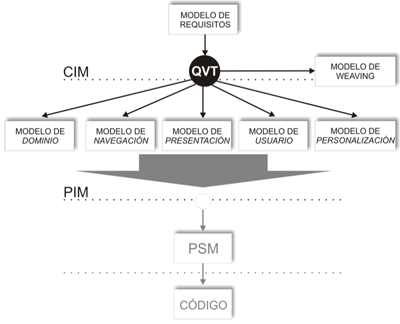
\includegraphics[width=0.8\textwidth]{img/approach.png}
\end{center}
\caption{La propuesta de la tesis doctoral integrada como CIM en el m�todo Web A-OOH.}
\label{fig:approach}
\end{figure}


\subsubsection{Especificaci�n del Modelo de Requisitos a Nivel CIM}\label{especificacion}

El primer paso de la propuesta presentada en la tesis doctoral es la especificaci�n y el modelado de los requisitos de la aplicaci�n Web. Para una explicaci�n m�s amplia el lector puede referirse al Cap�tulo \ref{c4} de la tesis doctoral.

Los requisitos Web se definen en un modelo independiente de computaci�n (CIM) utilizando el marco de modelado de requisitos \emph{i*}. El marco de modelado \emph{i*}  \cite{Yu95, Yu97} es uno de los m�s utilizados para analizar los objetivos de los \emph{stakeholder's} \footnote{Las personas u organizaciones que afectan o son afectados directa o indirectamente por el proyecto de desarrollo de \emph{software} en una forma positiva o negativa \cite{Sommerville96}.}, nombrados actores en \emph{i*}, y c�mo el sistema a dise�ar deber�a satisfacerlos. Adem�s, \emph{i*} permite razonar acerca de c�mo estos objetivos pueden contribuir a la selecci�n de diferentes alternativas de dise�o seg�n su viabilidad. Con el fin de motivar esta parte de la investigaci�n, se ha realizado una revisi�n del estado de la cuesti�n (ver Cap�tulo \ref{c3} y Ap�ndice~\ref{a1}) acerca de las t�cnicas utilizadas para el an�lisis y especificaci�n de requisitos en ingenier�a Web.

El marco de modelado \emph{i*} consiste b�sicamente en dos modelos: el modelo SD (\emph{Strategic Dependency}) para especificar las relaciones de dependencia entre varios actores en un contexto organizacional y el modelo SR (\emph{Strategic Rationale}), utilizado para describir los intereses y preocupaciones del actor y como es que podr�an abordarse. El modelo SR permite el modelado de las relaciones de asociaci�n entre cada actor y sus dependencias, por tanto, proporciona informaci�n acerca de c�mo los actores llegan a sus objetivos. El modelo SR incluye s�lo los elementos considerados lo suficientemente importantes como para influir en el alcance de un objetivo. El modelo SR muestra las dependencias de los actores mediante la inclusi�n del modelo SD. En torno a estas dependencias, el modelo SR especifica elementos intencionales, tales como (\emph{Goals}), tareas (\emph{Tasks}), recursos (\emph{Resources}) y \emph{Softgoals} (Tabla \ref{tab:istarsymbols}). En comparaci�n con el modelo SD, los modelos SR proporcionan un nivel de modelado m�s detallado, debido a que permiten modelar las relaciones internas e intencionales dentro de los actores. Las relaciones intencionales son enlaces del tipo \emph{Meands-end} y representan formas alternativas para satisfacer objetivos; los \emph{Decomposition-links} representan los elementos necesarios para que una tarea sea realizada; o los \emph{Contribution-links} que sirven para modelar c�mo es que un elemento intencional contribuye a la satisfacci�n de una (\emph{Softgoal}). En la Tabla \ref{tab:istarsymbols} se describen los elementos m�s importantes del marco de modelado \emph{i*}, para informaci�n m�s extendida el lector puede consultar \cite{istarWiki, Yu95, Yu97}. 

%\begin{table}
%\centering
%\tiny
%\caption{La notaci�n de \emph{i*}.}\label{tab:istarsymbols}
%\begin{tabular}{|c|c|c|c|}
%\hline
%\textbf{S�mbolo} & \textbf{Nombre} & \textbf{S�mbolo} & \textbf{Nombre}\\
%\hline
%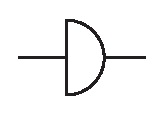
\includegraphics[height=3mm]{img/dependency.eps} & SD Model & 
\includegraphics[height=3mm]{img/boundary.eps} & SR Model\\
%
\includegraphics[height=3mm]{img/iactor.eps} & Actor & 
\includegraphics[height=3mm]{img/goal.eps} & Goal \\
%
\includegraphics[height=3mm]{img/task.eps} & Task & 
\includegraphics[height=3mm]{img/resource.eps} & Resource\\
%
\includegraphics[height=3mm]{img/softgoal.eps} & Softgoal & 
\includegraphics[height=3mm]{img/means-end.eps} & Means-end link\\
%
\includegraphics[height=3mm]{img/decomposition.eps} & Task-decomposition link & 
\includegraphics[height=3mm]{img/contribution.eps} & Contribution link\\
%\hline
%\end{tabular}
%\end{table}

\begin{table}
\caption{Principales elementos para el modelado en \emph{i*}}
\label{tab:istarsymbols}
\begin{tabular}{p{0.3\textwidth}p{0.2\textwidth}p{0.4\textwidth}}
\hline\noalign{\smallskip}
Elemento & Icono& Descripci�n  \\
\noalign{\smallskip}\hline\noalign{\smallskip}
\textsc{Actor} & (
\includegraphics[height=3mm]{img/iactor.eps}) & Es una entidad que lleva a cabo acciones para cumplir con sus objetivos. Se relaciona con varios elementos intencionales (objetivo, tarea o recurso).\\
\textsc{Goal} & (
\includegraphics[height=3mm]{img/goal.eps}) & Representa una condici�n o estado que el actor le gustar�a alcanzar. Lamentablemente no detalla como es que se satisfar� el objetivo.\\
\textsc{Task} & (
\includegraphics[height=3mm]{img/task.eps}) & Representa una manera particular de hacer algo (alcanzar un objetivo). \\
\textsc{Softgoal} & (
\includegraphics[height=3mm]{img/softgoal.eps}) & Representan criterios de calidad. Son utilizadas cuando los objetivos del \emph{stakeholder} no son precisos o sus criterios de �xito no est�n claramente definidos.\\
\textsc{Resource} & (
\includegraphics[height=3mm]{img/resource.eps}) & Es una entidad que debe estar disponible para su uso (datos).\\
\textsc{Means-ends} & (
\includegraphics[height=3mm]{img/means-end.eps}) & Son asociaciones que describen c�mo se alcanzan los objetivos, es decir, los posibles caminos para satisfacer un objetivo. \\
\textsc{Decomposition} & (
\includegraphics[height=3mm]{img/decomposition.eps}) & Son asociaciones que definen elementos adicionales necesarios para llevar a cabo una tarea. \\
\noalign{\smallskip}\hline\noalign{\smallskip}
\end{tabular}
\end{table}

Por otra parte, el marco de modelado \emph{i*} resulta insuficiente para representarlas por s� solo las caracter�sticas particulares de las aplicaciones Web, tales como el contenido que ofrecen, la navegaci�n, la funcionalidad y la audiencia heterog�nea (para m�s informaci�n consultar Cap�tulo \ref{c3} y Ap�ndice~\ref{a1}). Por tal motivo, \emph{i*} debe de adaptarse al dominio Web para poder ser utilizado en la especificaci�n y an�lisis de requisitos. Esto permitir� modelar a los \emph{stakeholders} con sus objetivos y las relaciones existentes entre ellos para satisfacerlos. Para realizar la adaptaci�n del marco de modelado \emph{i*} al dominio Web nuestra propuesta utiliza la taxonom�a de requisitos Web presentada en \cite{EscalonaK04}, la cual clasifica a los requisitos Web en 6 tipos. Estos son descritos a continuaci�n:

\begin{itemize}
   
   \item \textbf{Requisitos de contenido (\emph{Content})}. Con este tipo de requisitos se define el contenido que el sitio Web presenta a sus usuarios. Considerando como ejemplo base una librer�a \emph{on-line}, algunos ejemplos pueden ser:  ``informaci�n del libro'' o ``categor�as del producto''.
  
   \item \textbf{Requisitos de servicio (\emph{Service})}. Este tipo de requisito hace referencia a la funcionalidad interna que la aplicaci�n Web debe proveer a los usuarios. Continuando con el ejemplo de la librer�a \emph{on-line}, ejemplo de requisitos de servicio son: ``registrar un nuevo cliente'', ``agregar un producto'', etc.
   
   \item \textbf{Requisitos de navegaci�n (\emph{Navigational})}. Un sistema Web debe tambi�n definir caminos de navegaci�n disponibles para los usuarios. Algunos ejemplos, en base a la librer�a \emph{on-line} son: ``consultar productos por categor�a'', ``consultar el carrito de compras'', etc.
   
   \item \textbf{Requisitos de interfaz (\emph{Layout})}. Los requisitos tambi�n pueden definir la interfaz visual para los usuarios. Por ejemplo: ``presentar un estilo diferente para los adolescentes''.
   
   \item \textbf{Requisitos de personalizaci�n (\emph{Personalization})}. El dise�ador puede especificar las acciones de personalizaci�n a ser ejecutadas en el sitio Web. Por ejemplo: ``adaptar el estilo de la fuente para las personas con deficiencia visual''.
   
   \item \textbf{Requisitos no funcionales (\emph{Non-functional requirements})}. Estos requisitos representan criterios de calidad que el sistema debe conseguir. Algunos ejemplos de estos requisitos pueden ser: ``eficiencia'', ``atraer m�s usuarios'' y ``buena experiencia del usuario''.
\end{itemize}

Finalmente, para poder utilizar el marco de modelado \emph{i*} dentro de MDA se ha implementado un metamodelo. El metamodelo se implement� utilizando la tecnolog�a EMF (\emph{Eclipse Modeling Framework}) de Eclipse \cite{ECLIPSE} (Fig. \ref{fig:SeccionRequisitosWebMetamodelo}). Los elementos intencionales de \emph{i*} fueron extendidos con nuevas clases para representar cada uno de los tipos de requisitos Web descritos anteriormente (\emph{Navigational}, \emph{Service}, \emph{Personalization}, \emph{Layout} y \emph{Content}). De esta forma, los requisitos \emph{Navigational}, \emph{Service}, \emph{Personalization} y \emph{Layout} son instancias del elemento \emph{Task} del marco de modelado \emph{i*}, por lo tanto, se representar�n visualmente por medio de la figura (
\includegraphics[height=3mm]{img/task.eps}) y el requisito \emph{Content}, del elemento \emph{Resource}, ser� representado por la forma (
\includegraphics[height=3mm]{img/resource.eps}) de \emph{i*}. 

Por �ltimo, es importante destacar que los requisitos no-funcionales de la aplicaci�n Web se modelan directamente utilizando el elemento \emph{Softgoal}, por tanto, cuando se lleve a cabo la especificaci�n de requisitos utilizando esta propuesta, el concepto de requisito no-funcional corresponder� al concepto de \emph{Softgoal} del marco de modelado \emph{i*} y se representar� visualmente con la imagen (
\includegraphics[height=3mm]{img/softgoal.eps}). 

%\begin{figure}
%\begin{center}
%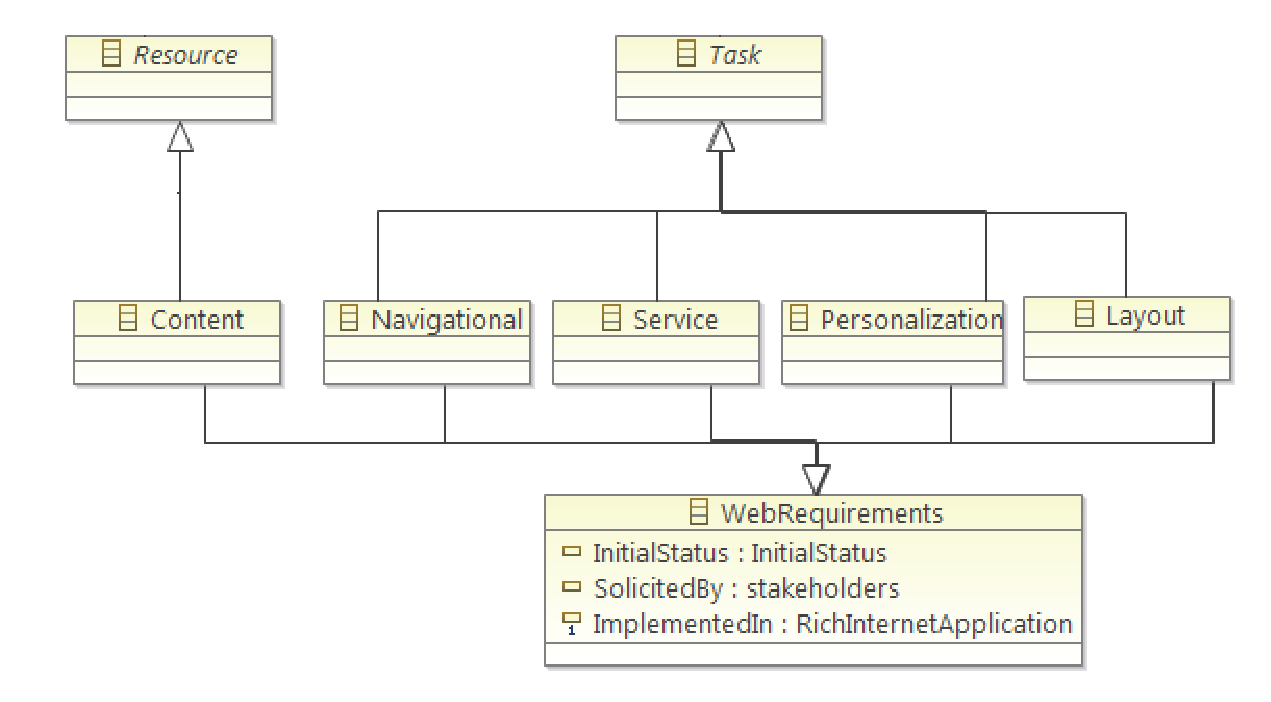
\includegraphics[width=\textwidth]{img/SeccionRequisitosWebMetamodelo.eps}
%\end{center}
%\caption{Extracto de metamodelo de requisitos Web del m�todo A-OOH.}
%\label{fig:reqmetamodel}
%\end{figure}
\begin{landscape}
\begin{figure}
\begin{center}
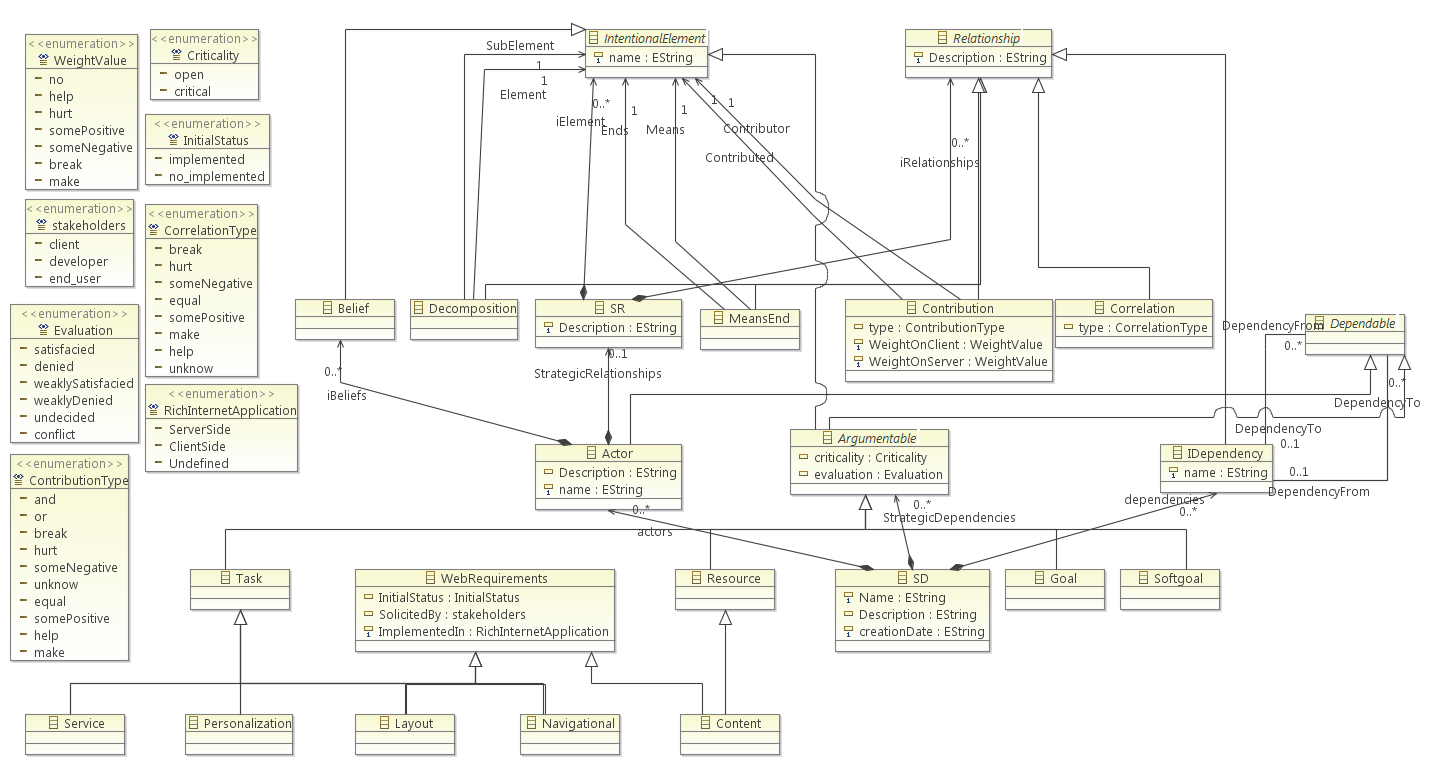
\includegraphics[width=1.8\textwidth]{img/WebRequirementsMetamodel.png}
\end{center}
\caption{Metamodelo para la especificaci�n de requisitos Web con \emph{i*}.}
\label{fig:SeccionRequisitosWebMetamodelo}
\end{figure}
\end{landscape}

A continuaci�n, se resume la generaci�n de la estructura de los modelos conceptuales de A-OOH. Se remite al lector a los cap�tulos
espec�ficos de la tesis doctoral para una explicaci�n m�s detallada (Cap�tulo \ref{c4}).

%dominio y navegaci�n

\subsubsection{Generaci�n de los Modelos Conceptuales a nivel PIM}\label{reglas}

Definidos los requisitos en un CIM, el siguiente paso consiste en utilizarlos para derivar la estructura de los modelos conceptuales de la aplicaci�n Web. Para lograrlo, es necesario que los modelos cumplan con la sintaxis abstracta de un dominio especifico, es decir, que sean conformes a un metamodelo. A continuaci�n se describen los metamodelos utilizados para la derivaci�n de los modelos conceptuales a nivel PIM de MDA.

UML (\emph{Unified Modeling Language}) \cite{UML} es el lenguaje de modelado est�ndar utilizado para la derivaci�n del modelo de dominio de A-OOH. El metamodelo describe los objetos, atributos y relaciones necesarias para representar los conceptos de UML dentro de una aplicaci�n de \emph{software}. Los modelos est�ticos son presentados en diagramas llamados Diagramas de Clases. El prop�sito de un diagrama de clases es representar a las clases dentro de un modelo. En una aplicaci�n orientada a objetos, las clases tienen atributos (variables miembros), operaciones (funciones miembro) y relaciones con otras clases. Estas caracter�sticas aplican perfectamente para la representaci�n del modelo de dominio de A-OOH.

Por otra parte, A-OOH dispone de un metamodelo \cite{irene08} para representar las rutas de navegaci�n que el usuario puede seguir durante su interacci�n con la aplicaci�n Web. En la Figura \ref{fig:NavMetamodel} se muestra el metamodelo de navegaci�n utilizado en A-OOH. Los elementos principales del metamodelo son: (i) Nodo Navegacional (\emph{Navigational Node}) y (ii) Enlace Navegacional (\emph{Navigational Link}).


El Nodo Navegacional representa vistas restringidas de los conceptos del dominio y sus relaciones indican las rutas de navegaci�n que el usuario de la aplicaci�n Web puede seguir. Existen tres tipos diferentes de Nodos Navegacionales, los cuales se describen a continuaci�n:

\begin{itemize}
\item \textbf{Clases de Navegaci�n} (\emph{Navigational Classes}), son clases del dominio enriquecidas con atributos y m�todos cuya visibilidad ha sido restringida, dependiendo de los permisos de acceso del usuario y de los requisitos de navegaci�n. Es representada por una clase UML estereotipada como \emph{NavigationalClass}.

\item \textbf{Objetivos de Navegaci�n} (\emph{Navigational Targets}), agrupan los elementos del modelo que colaboran en el cumplimiento de cada requisito de navegaci�n del usuario. Son representados utilizando la notaci�n UML de paquetes con el estereotipo \emph{NavigationalTarget}.

\item \textbf{Colecciones} (\emph{Collections}), son estructuras jer�rquicas definidas en Clases Navegacionales u Objetivos Navegacionales. Proveen al usuario de la aplicaci�n Web nuevas formas de accesar a la informaci�n. La colecci�n m�s com�n es \emph{C-Collection} (\emph{Clasifier Collection}), la cual act�a como un mecanismo de abstracci�n para el concepto de \emph{men�}, agrupa de esta forma Enlaces Navegacionales (\emph{Navigational Links}). Otra colecci�n importante es la llamada \emph{S-Collection} (\emph{Selector Collection}) mediante la cual podemos representar un mecanismo de selecci�n. Las colecciones son representadas por medio de una clase UML estereotipada como \emph{NavigationalC-Collection} o \emph{NavigationalS-Collection}.
\end{itemize}

\begin{landscape}
\begin{figure}
\begin{center}
%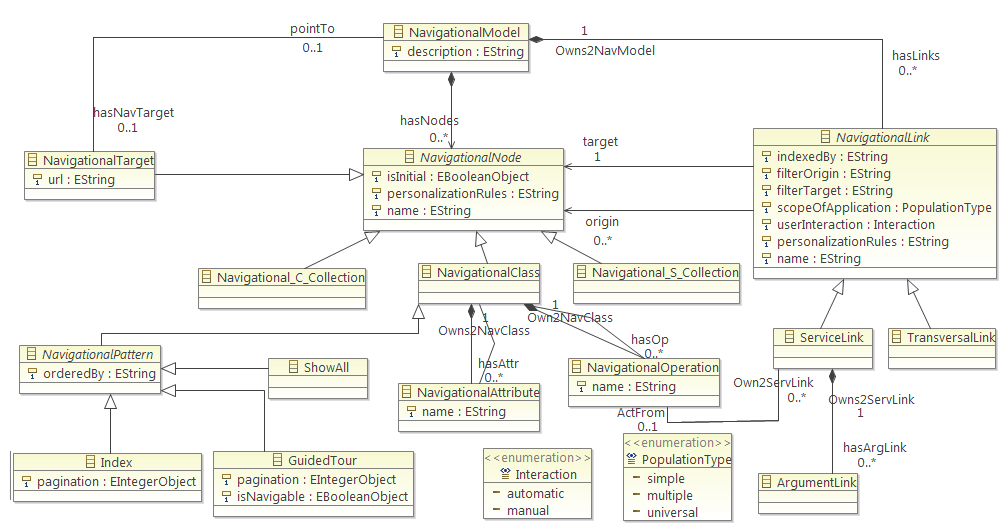
\includegraphics[width=1.5\textwidth]{img/NavigationalMetamodel.png}
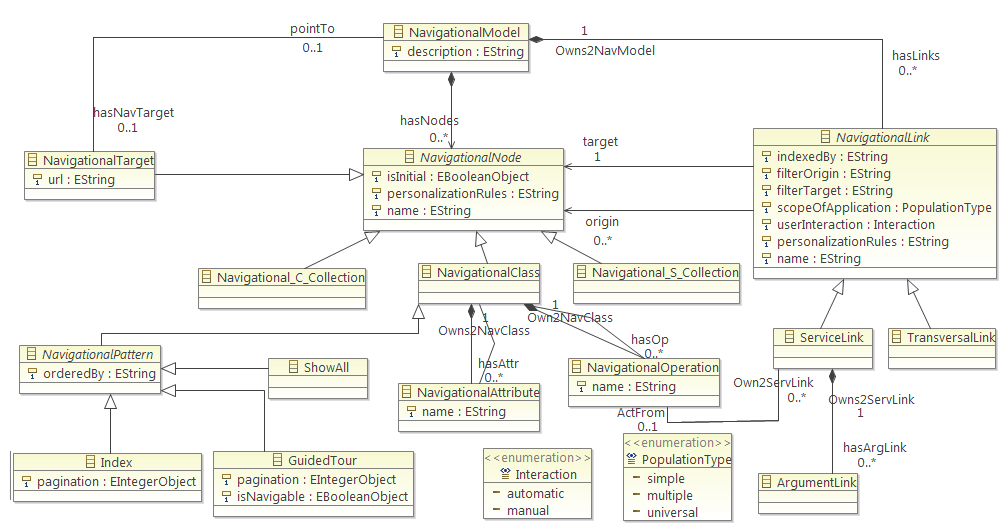
\includegraphics[width=18.5cm,height=13.5cm]{img/NavigationalMetamodel.png}
\end{center}
\caption{Metamodelo de Navegaci�n de A-OOH.}
\label{fig:NavMetamodel}
\end{figure}
\end{landscape}


El Enlace Navegacional define las rutas de navegaci�n que el usuario puede seguir a trav�s de la aplicaci�n Web. A-OOH en su metamodelo de navegaci�n define dos tipos principales de enlaces (\emph{links}):

\begin{itemize}
\item \textbf{T-Links} (\emph{Transversal Links}), son enlaces definidos entre dos nodos navegacionales (clases navegacionales, colecciones u objetivos navegacionales). La navegaci�n es realizada para mostrar informaci�n a trav�s de la interfaz del usuario sin modificar en absoluto la l�gica de negocio. Estos tipos de enlaces son representados por el estereotipo \emph{TransversalLink}.

\item \textbf{S-Link} (\emph{Service Links}), con estos tipos de enlaces la navegaci�n es realizada para activar una operaci�n, la cual, en forma opuesta a los \emph{T-Links} modifica la l�gica del negocio y adem�s implica que la navegaci�n a un nodo muestre informaci�n cuando termine la ejecuci�n del servicio. Se establece cuando un servicio de la clase navegacional es activado. Estos tipos de ligas son representados por el estereotipo \emph{ServiceLink}  y tiene asociado el nombre del servicio que lo invoco.
\end{itemize}


%Un modelo representa alg�n aspecto de un sistema \emph{software} y conforma con el metamodelo con el que est� expresado. Una vez se han presentado y descrito los metamodelos utilizados por A-OOH se proceder� a explicar la derivaci�n de los modelos conceptuales de dominio y navegaci�n.

Una vez han sido explicados los metamodelos de dominio y navegaci�n de A-OOH, el siguiente paso consiste en describir sus respectivos modelos. El modelo de dominio en A-OOH encapsula la estructura y funcionalidad de los conceptos relevantes del dominio de la aplicaci�n Web y tambi�n refleja la parte est�tica de la misma, se representa como un diagrama de clases en notaci�n UML \cite{UML}. El objetivo consiste en obtener el esqueleto del modelo de dominio de A-OOH a partir del modelo de requisitos en \emph{i*} por medio de un conjunto de reglas de transformaci�n modelo a modelo (M2M) \cite{OMG/QVT} (ver Cap�tulo \ref{4} y Ap�ndice \ref{a3}). 

%Con las reglas, se obtendr� un modelo de \emph{weaving} para mantener enlaces bidireccionales entre los elementos de ambos modelos (a nivel de sus respectivos elementos). A continuaci�n se describen las principales reglas QVT para generar el modelo de dominio y el modelo de \emph{weaving}:

\begin{itemize}
\item \textbf{\emph{Content2DomainClass}}. El dominio origen de la relaci�n est� compuesto por un conjunto de elementos que representan un requisito del tipo \emph{Content}. Cuando se detecta este patr�n en el modelo de entrada se fuerza la creaci�n de una clase tipo \emph{Class UML} en el modelo destino (modelo de dominio). Por tanto, por cada requisito de contenido, se obtiene una clase en el modelo de dominio (Figura \ref{fig:content2Domain}).

\begin{figure}
\begin{center}

\includegraphics[width=0.8\textwidth]{img/content2domainclass.eps}
\end{center}
\caption{Regla QVT para obtener las clases del modelo de dominio.}
\label{fig:content2Domain}
\end{figure}

\item \textbf{\emph{Service2Operation}}. La regla detecta un conjunto de elementos en el modelo de entrada (modelo de requisitos) que corresponden con un requisito \emph{Service} asociado a un requisito \emph{Content}. Una vez detectado este patr�n de elementos, se crea en el modelo de salida (modelo de dominio) una clase \emph{Operation} en la clase del modelo de dominio correspondiente (Figura \ref{fig:service2operation}).

\begin{figure}
\begin{center}

\includegraphics[width=0.8\textwidth]{img/service2operation.eps}
\end{center}
\caption{Regla QVT para obtener las operaciones de las clases del modelo de dominio.}
\label{fig:service2operation}
\end{figure}

\item \textbf{\emph{Navigation2Relationship}}. Esta relaci�n permite crear asociaciones entre clases en el modelo de dominio. Existen dos requisitos \emph{Content} como origen, si los dos requisitos se usan para cumplir el mismo requisito de navegaci�n, entonces se crea una clase \emph{Association} entre las clases del modelo de dominio que las representan (Figura \ref{fig:navigation2relationship}).

\begin{figure}
\begin{center}

\includegraphics[width=0.8\textwidth]{img/navigation2relationship.eps}
\end{center}
\caption{Regla QVT para obtener las relaciones entre las clases del modelo de dominio A-OOH.}
\label{fig:navigation2relationship}
\end{figure}
\end{itemize}


Como se mencion� anteriormente, el modelo de navegaci�n est� compuesto de nodos navegacionales y sus respectivas relaciones para indicar las rutas de navegaci�n de la aplicaci�n Web. Para derivar el modelo de navegaci�n los requisitos tomados en cuenta para generar un conjunto de reglas de transformaci�n QVT son los requisitos de contenido (\emph{Content}), servicio (\emph{Service}), navegaci�n (\emph{Navigational}) y personalizaci�n (\emph{Personalization}). En este caso, las reglas QVT para la obtenci�n del modelo de navegaci�n son las siguientes:


\begin{itemize}

\item \textbf{\emph{Navigation2NavClass}}. La regla de transformaci�n detecta cada requisito navegacional, derivando su correspondiente clase. En concreto, cuando se detecta en el modelo origen un requisito \emph{Navigational} unido a un requisito \emph{Content}, entonces se crea una clase estereotipada como \emph{NavigationalClass} en el modelo destino. Adem�s cada una de las nuevas clases es el destino de una nueva asociaci�n \emph{TransversalLink} desde una \emph{C-Collection} previamente creada por la funci�n \emph{createMenu} que se encuentra en la cl�usula \emph{when} (Figura \ref{fig:nav2navclass}).

\begin{figure}
\begin{center}

\includegraphics[width=0.8\textwidth]{img/nav2navclass.eps}
\end{center}
\caption{Regla QVT para obtener las clases navegacionales.}
\label{fig:nav2navclass}
\end{figure}

\item \textbf{\emph{Personalization2NavClass}}. La regla es similar a la anterior pero detectando los requisitos de personalizaci�n que tienen un requisito de contenido asociado. Se derivan en el modelo de navegaci�n los mismos elementos que en la regla anterior.


\item \textbf{\emph{Navigation2TransversalLink}}. Permite crear asociaciones entre clases navegacionales en el modelo de navegaci�n. Existen dos modelos origen con el fin de detectar requisitos \emph{Content}, si los dos requisitos se usan para cumplir con el mismo requisito de navegaci�n (comprobado en la cl�usula \emph{when} con la operaci�n \emph{SameNavigationOrigin)}, entonces se crea una asociaci�n \emph{TransversalLink} entre las clases del modelo de navegaci�n que las representan.

\item \textbf{\emph{Service2ServiceAndSLink}}. La relaci�n detecta un conjunto de elementos en el modelo origen que corresponden con un requisito \emph{Service} asociado a un requisito \emph{Content}. Una vez detectado este patr�n de elementos, se crea en el modelo destino una clase \emph{Operation} en la clase del modelo de navegaci�n correspondiente. Adem�s, se crea una asociaci�n \emph{ServiceLink} para cada operaci�n a�adida. El nuevo enlace de servicio se asocia a una nueva clase navegacional (\emph{NavigationalClass}) destino. Antes de ejecutarse la transformaci�n, se debe verificar que se cumple con las sentencias dispuestas en la cl�usula \emph{when}, en este caso \emph{Navigation2NavClass} y \emph{Personaliza tion2NavClass}, con el fin de crear en el modelo destino todas las posibles clases de navegaci�n a partir de cada uno de los requisitos \emph{Content} en el modelo origen.


\end{itemize}

Finalmente, es importante mencionar que los modelos conceptuales derivados son modelos iniciales que servir�n como punto de partida para el dise�ador Web, de esta forma es posible proveer un alto grado de automatizaci�n en el proceso de desarrollo de aplicaciones Web dirigido por modelos.

\subsection{Gesti�n de Requisitos en A-OOH}
\label{c1:gestion}

Las metodolog�as para el desarrollo de aplicaciones Web a�n no responden a las exigencias actuales de este tipo de \emph{software} \cite{Aguilar2010}. En ese aspecto, las necesidades y expectativas de los \emph{stakeholders} no son captadas satisfactoriamente. De ah� que una considerable cantidad de proyectos de desarrollo no alcancen a cumplir sus objetivos, y como consecuencia de esto, la aplicaci�n Web no cumple con las expectativas reales de los usuarios \ref{BolchiniP04, Bolchini2003, EscalonaK04}. 

Las principales causas de estos problemas son la gesti�n insuficiente de los requisitos funcionales y no-funcionales, la comunicaci�n ambigua e imprecisa entre los \emph{stakeholders}, las inconsistencias no detectadas entre los requisitos, dise�o y programaci�n, as� como la propagaci�n de cambios sin analizar su impacto. En este sentido, es necesario recordar que los errores m�s comunes y m�s costosos de reparar, as� como los que m�s tiempo consumen, se deben a una inadecuada ingenier�a de requisitos. Actividades propias de esta �rea, como la especificaci�n o la gesti�n de requisitos, son algunas de las consideradas m�s cr�ticas en ingenier�a Web y en la ingenier�a de \emph{software} en general.

Por otra parte, el uso de t�cnicas orientadas a objetivos \cite{Yu95} para la especificaci�n de requisitos en ingenier�a Web \cite{Bolchini2003, Garrigos09} permite reflejar desde las etapas iniciales del proceso de desarrollo los objetivos, tareas y relaciones de los \emph{stakeholders}, lo que proporciona los elementos necesarios para que se consideren las necesidades y objetivos del usuario de la aplicaci�n Web. Sin embargo, a pesar de que los requisitos son especificados en un modelo conceptual, los \emph{stakeholders} necesitan observar que han sido reflejados correctamente en la aplicaci�n Web final. Una forma de brindar soporte a esta necesidad es proveer al dise�ador Web con una etapa de requisitos que considere la gesti�n de los mismos.


Por tanto, la propuesta presentada en la tesis se ha extendido para proveer al dise�ador con soporte para: (i) trazabilidad de requisitos (CIM-PIM) \cite{aguilarDSDM} (Ap�ndice \ref{a3}), (ii) evaluar el impacto derivado de un cambio en los modelos conceptuales (an�lisis de impacto) \cite{AguilarICCSA} (Cap�tulo \ref{c5}) y (iii) seleccionar alternativas de dise�o considerando la maximizaci�n y/o balance de los requisitos no-funcionales \cite{AguilarWISM} (Cap�tulo \ref{c6}).

\subsubsection{Trazabilidad de Requisitos en A-OOH}
\label{c1:trazabilidad}

En el campo de la ingenier�a Web dirigida por modelos, realizar el seguimiento de los requisitos durante la etapa de desarrollo de la aplicaci�n Web hasta su implementaci�n final es una tarea compleja \cite{AguilarICCSA}. Esto se debe a que en ingenier�a Web se deben generar varios modelos conceptuales a partir de los requisitos como son el modelo de dominio o de navegaci�n. Adem�s, debido al desarrollo gradual de las necesidades de los usuarios de la aplicaci�n Web, los modelos cambian constantemente, por lo que la trazabilidad de los requisitos se hace indispensable.

La trazabilidad de requisitos se define como la capacidad de describir y seguir la vida de un requisito, en ambas direcciones \cite{gotel1994analysis}: (i) determinar qu� partes del modelo est�n relacionadas con cada uno de los requisitos, y (ii) determinar qu� requisitos dieron origen a qu� partes del modelo. En la actualidad, existen dos estrategias para gestionar y almacenar la informaci�n para la trazabilidad entre modelos: (i) la informaci�n se puede integrar en los modelos a los que se refiere y (ii) la informaci�n de trazabilidad se puede almacenar por separado en otro modelo \cite{barbero2007traceability}. La primera de estas dos opciones tiene como desventaja que si la informaci�n es almacenada en el mismo modelo, el modelo ser� contaminado con informaci�n poco relevante para el contexto del modelo y por lo tanto, ser� dif�cil de mantener y utilizar. Por otro lado, la segunda estrategia consiste en almacenar la informaci�n en un modelo aparte. De esta forma se pueden corregir las desventajas mencionadas.

Con el fin de brindar soporte para la trazabilidad de requisitos en A-OOH \cite{aguilarDSDM} se ha utilizado el concepto de modelo de \emph{weaving}. Un modelo de \emph{weaving} es un tipo de modelo formado por enlaces y referencias a elementos, los enlaces est�n dirigidos a las referencias de los elementos de un modelo origen y de un modelo destino \cite{bezivin2005unification}. A continuaci�n, se presenta el metamodelo base para \emph{weaving} \cite{del2006weaving} y una extensi�n para proveer a dicho metamodelo con elementos �tiles para representar la trazabilidad entre modelos \cite{barbero2007traceability}. El metamodelo se muestra en la Figura \ref{fig:weavingmetamodel}:

\begin{itemize}
\item \textbf{\emph{WElement}}. Es el elemento base del cual los elementos restantes heredan, esta formado por los atributos nombre y descripci�n.
\item \textbf{\emph{WModel}}. Representa el elemento ra�z que contiene a todos los elementos del modelo. Est� compuesto por las referencias y relaciones a los modelos de entrada y salida.
\item \textbf{\emph{WLink}}. Sirve para representar un enlace entre los elementos de los modelos de entrada y salida.
\item \textbf{\emph{WLinkEnd}}. Este elemento representa la referencia origen o destino de un \emph{WLink}.
\item \textbf{\emph{WElementRef}}. Este elemento se asocia a una funci�n de identificaci�n, creando un identificador �nico para cada uno de elementos de los modelos de entrada y salida, por tanto \emph{WElementRef} permite referenciar el mismo elemento de los modelos de entrada y salida por diversos elementos \emph{WLinkEnd}.
\item \textbf{\emph{WModelRef}}. Representa un identificador �nico de un modelo.
\end{itemize}

%\begin{landscape}
\begin{figure}
\begin{center}
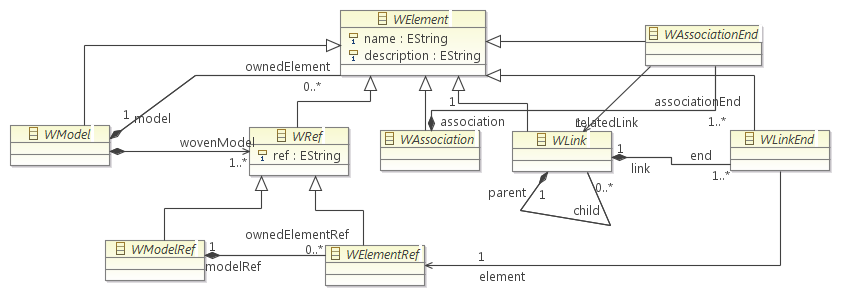
\includegraphics[width=\textwidth]{img/WeavingMetamodel.png}
\end{center}
\caption{Metamodelo de \emph{weaving}.}
\label{fig:weavingmetamodel}
\end{figure}
%\end{landscape}


Por otra parte, en la Figura \ref{fig:tracemetamodel}, se ilustra la extensi�n del metamodelo para \emph{weaving} que permite la representaci�n de la trazabilidad. La extensi�n la forman los siguientes elementos:

\begin{itemize}
\item \textbf{\emph{TraceModel}}. Es el elemento que representa al modelo de trazabilidad, est� integrado por referencias a otros modelos.
\item \textbf{\emph{TraceModelRef}}. Representa la referencia a otros modelos, es decir, es un �nico identificador para los modelos que conforman el modelo de trazabilidad.
\item \textbf{\emph{ElementRef}}. Es un identificador para se�alar cada elemento que integran los modelos ligados.
\item \textbf{\emph{TraceLink}}. Un enlace de rastreo, utilizado para representar las correspondencias entre las referencias de los elementos de los modelos enlazados. Como informaci�n de trazabilidad, almacena el nombre de la regla de transformaci�n que ha sido ejecutada.
\item \textbf{\emph{TraceLinkEnd}}. Su funci�n es similar al elemento \emph{WLinkEnd} del cual hereda, pues permite crear una relaci�n uno a muchos (1-N) entre las referencias de los elementos del modelo de entrada (\emph{sourceElements}) y los del modelo de salida (\emph{targetElement}).
\end{itemize}

%\begin{landscape}
\begin{figure}
\begin{center}
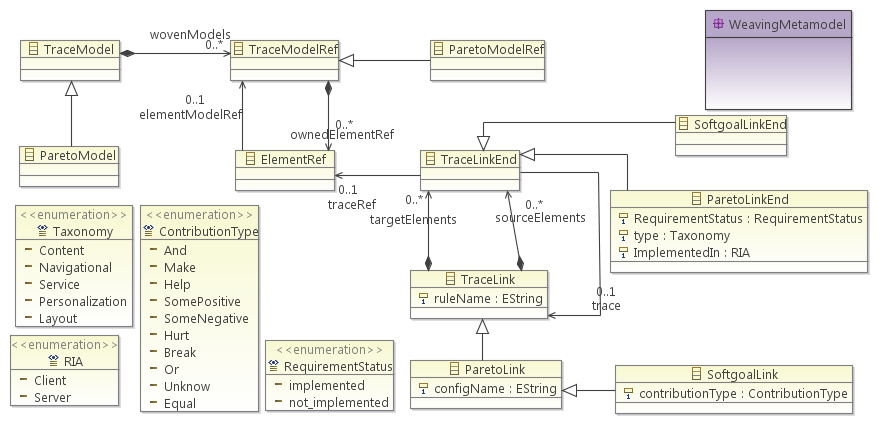
\includegraphics[width=\textwidth]{img/TraceabilityMetamodel.png}
\end{center}
\caption{Extensi�n del metamodelo de \emph{weaving} para trazabilidad.}
\label{fig:tracemetamodel}
\end{figure}
%\end{landscape}

Los \emph{trace links} han sido introducidos dentro de las reglas de transformaci�n que generan los elementos de los modelos conceptuales de A-OOH. Asimismo, es generado un modelo de trazabilidad (\emph{trace model}) al ejecutarse el conjunto de transformaciones por primera vez. Para un mejor entendimiento, se ha utilizado el lenguaje est�ndar QVT \cite{QVT-OMG} para representar en la Figura \ref{fig:Content2DomainWithTrace} la incorporaci�n de los \emph{trace links} dentro de la regla \emph{Content2DomainClass}. En la figura, se observa que por cada vez que se encuentre un requisito \emph{Content} en el modelo de entrada (modelo de requisitos \emph{i*}), se crear� en el modelo de dominio una clase del tipo \emph{Class} de UML, y al mismo tiempo, para referenciar a los elementos de los modelos de entrada y salida, se crear� un (\emph{trace link}) en el modelo de trazabilidad.

%\begin{landscape}
\begin{figure}
\begin{center}
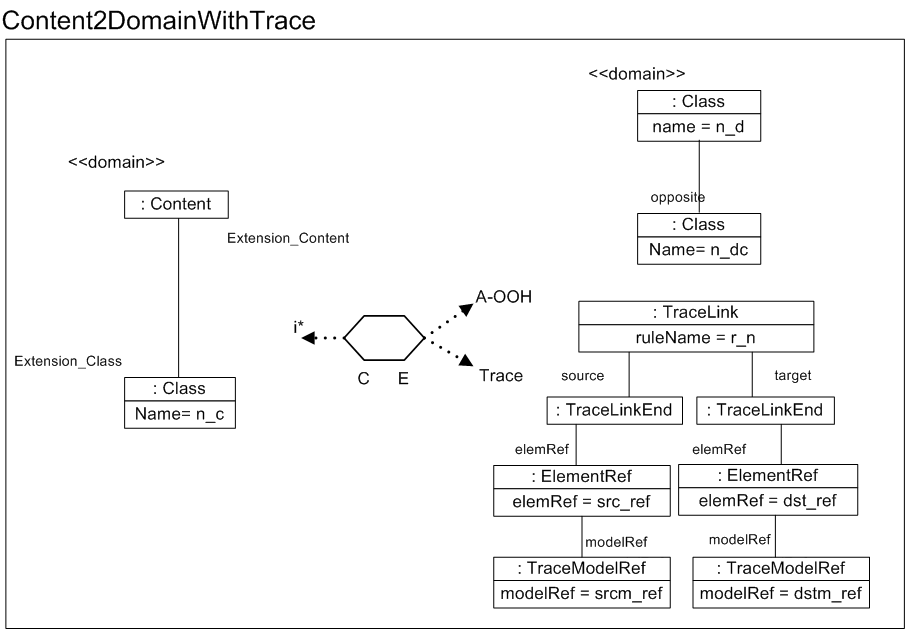
\includegraphics[width=0.8\textwidth]{img/Content2DomainWithTrace.png}
\end{center}
\caption{Incorporaci�n de los (\emph{trace links}) en la generaci�n de los modelos conceptuales de A-OOH.}
\label{fig:Content2DomainWithTrace}
\end{figure}
%\end{landscape}

\subsubsection{An�lisis de Impacto en A-OOH}
\label{c1:analisisimpacto}

Los requisitos evolucionan constantemente a raz�n de la naturaleza din�mica de la Web. Debido a esto, es com�n encontrar inconsistencias entre los modelos conceptuales de la aplicaci�n Web y los requisitos. Una de las ventajas ofrecidas por el soporte para trazabilidad en A-OOH es el de conocer las dependencias entre los elementos de los modelos conceptuales y los requisitos. Por tanto, es posible conocer los requisitos afectados debido a un cambio en alguno de los modelos conceptuales. 

An�lisis de impacto, conocido tambi�n como (\emph{Change Impact Analysis}), es la tarea de identificar las consecuencias potenciales de un cambio o estimar qu� es necesario modificar para llevar a cabo el cambio \cite{impact}, por ejemplo, una modificaci�n en los modelos conceptuales de la aplicaci�n Web o en la especificaci�n de los requisitos. Com�nmente, el an�lisis de impacto se ha realizado de forma intuitiva por los dise�adores de la aplicaci�n Web por medio de un an�lisis superficial del c�digo y documentaci�n de la aplicaci�n. Esto quiz� sea suficiente para aplicaciones Web no muy grandes, pero no es suficientes para aplicaciones Web sofisticadas. Asimismo, trabajos de investigaci�n emp�rica como el presentado en \cite{Lindvall} y m�s recientemente en \cite{goeritzer2011usingImpactAna}, demuestran que incluso los desarrolladores m�s experimentados en la industria, deducen un an�lisis de impacto incompleto.

Para paliar esta limitante, se ha definido un algoritmo para analizar las dependencias entre los requisitos funcionales. El algoritmo analiza el modelo de requisitos para conocer las dependencias entre los requisitos funcionales adem�s de saber qu� requisitos no-funcionales se ven afectados (ver Cap�tulo \ref{c5}). De esta forma, a trav�s del soporte para trazabilidad es posible conocer que otros elementos de los modelos conceptuales son afectados debido a un cambio en la aplicaci�n Web. Finalmente, debido a que el modelo de requisitos es orientado a objetivos \cite{AguilarJUCS, Garrigos09}, el algoritmo puede mostrar al dise�ador un camino alternativo en el cual se indique qu� requisitos funcionales tienen que ser implementados para seguir cumpliento con el objetivo (\emph{Goal}). A continuaci�n se presenta un ejemplo de la aplicaci�n del algoritmo.

Supongamos que el cliente ha solicitado la implementaci�n de una aplicaci�n Web que permita la aplicaci�n de encuestas \emph{on-line}. En primer lugar es necesario que el dise�ador especifique los requisitos de la aplicaci�n Web, para esta demostraci�n, solo se ha definido el actor que representa a la aplicaci�n Web (Figura \ref{fig:req1iccsa}). 

\begin{figure}
\begin{center}
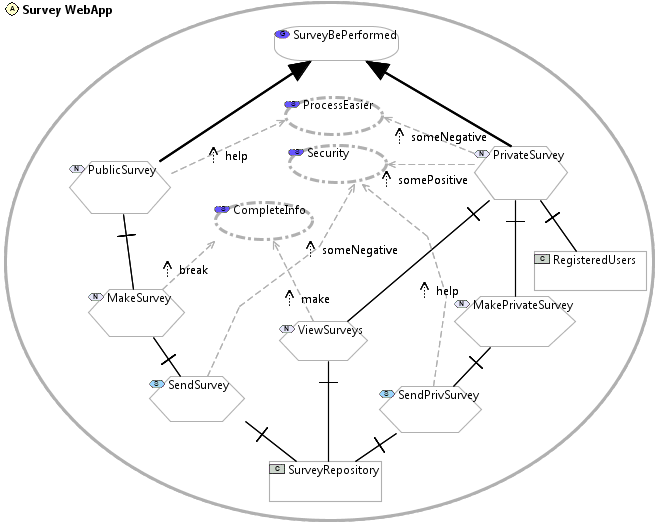
\includegraphics[width=0.8\textwidth]{img/EjemploICCSA.png}
\end{center}
\caption{El modelo de requisitos de la aplicaci�n \emph{``Survey WebApp''}.}
\label{fig:req1iccsa}
\end{figure}

El actor ``\emph{Survey WebApp}'' tiene que cumplir con el objetivo ``\emph{Survey be performed}'', para lograrlo dispone de dos v�as, por medio de la aplicaci�n de la encuesta p�blica ``\emph{Public survey}'' o la privada ``\emph{Private survey}'', ambos requisitos de navegaci�n. Cada una de las v�as necesita de uno o m�s requisitos para cumplirse, tal es el caso del requisito ``\emph{Private survey}'' debido a que necesita de los requisitos de navegaci�n ``\emph{Make private survey}'' y ``\emph{View survey}'' as� como del requisito de contenido ``\emph{Registered users}''. 

En este sentido, algunos de los requisitos afectan positiva o negativamente a las \emph{Softgoals}, por ejemplo, el requisito navegacional ``\emph{Private survey}'' afecta positivame a la \emph{Softgoal} ``\emph{Security}'' (encargada de la seguridad de la aplicaci�n Web), pero tambi�n afecta de forma negativa a la \emph{Softgoal} ``\emph{Process Easier}'', la cual representa el nivel de simplicidad con que deber� realizarse el proceso de revis�n utilizando la aplicaci�n Web (usabilidad), por �ltimo, el requisito navegacional ``\emph{View Surveys}'' afecta de forma positiva a la \emph{Softgoal} ``\emph{Complete Info}'', es decir que si este requisito navegacional es implementado, el usuario de la aplicaci�n Web podr� obtener informaci�n m�s detallada acerca del art�culo asignado para su revisi�n.


El tipo de contribuciones que realizan los requisitos funcionales a las \emph{Softgoals} es relevante para la ejecuci�n del algoritmo a raz�n de que son utilizadas para decidir qu� requisitos funcionales ser� necesario implementar. En el ejemplo, solo los requisitos funcionales relacionados con el requisito de navegaci�n ``\emph{Public survey}'' se encuentran implementados en los modelos conceptuales (Figura \ref{fig:req1iccsaIniciales}). 

\begin{figure}
\begin{center}
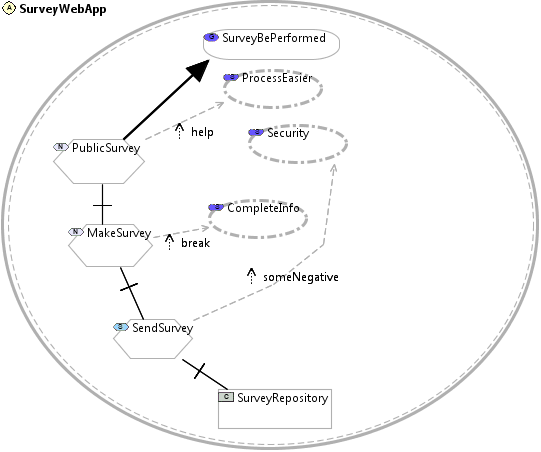
\includegraphics[width=0.8\textwidth]{img/EjemploICCSAReqIniciales.png}
\end{center}
\caption{Requisitos de la aplicaci�n \emph{``Survey WebApp''} implementados inicialmente.}
\label{fig:req1iccsaIniciales}
\end{figure}

Ahora bien, supongamos el siguiente escenario: se presenta una solicitud de cambio en la estructura de la base de datos de la aplicaci�n Web, por tal motivo, el dise�ador Web necesita eliminar un elemento del modelo de dominio A-OOH, gracias al soporte para trazabilidad, es posible conocer el requisito afectado por la clase del modelo de dominio que ha sido eliminada, como puede verse en la Figura \ref{fig:req1iccsaIniciales}, la clase corresponde con el requisito navegacional ``\emph{Public survey}''. Por tanto, el objetivo ``\emph{Survey be performed}'' no se puede cumplir. Por tal motivo, es necesario conocer:

\begin{itemize}
	\item �Qu� requisitos son afectados por este cambio en el modelo de requisitos?
	\item �Qu� elementos de los modelos conceptuales son afectados?
\end{itemize}

Por �ltimo, es necesario encontrar un camino alternativo en el modelo de requisitos (si es que existe) para continuar cumpliendo con el objetivo ``\emph{Survey be performed}''.

El algoritmo inicia una vez que se han cumplido un conjunto de pre-condiciones, las cuales pueden consultarse con detalle en el Cap�tulo \ref{c5}. El primer paso del algoritmo consiste en realizar un listado de todos aquellos requisitos funcionales que se encuentren implementados o no (en este caso, reflejados en el modelo de dominio), y que adem�s realicen alguna contribuci�n positiva o negativa a cualquier \emph{Softgoal}, el listado quedar� como lo muestra la Tabla \ref{tab:listaElementosIntencionales1}. El requisito afectado se muestra resaltado en negrita. Con el listado generado y el soporte para trazabilidad de A-OOH, es posible saber qu� elementos del modelo conceptual de dominio resultan afectados por la eliminaci�n del requisito navegacional ``\emph{Public survey}''.

\begin{table}
 \centering
%\tiny %\addtolength{\tabcolsep}{-5pt}
 \caption{La contribuci�n de los requisitos funcionales a cada requisito no-funcional.}\label{tab:listaElementosIntencionales1}
\begin{tabular}{| l | c| c | c |}
\hline
\textbf{Requirements} &
\textbf{\emph{``Process easier''}} &
\textbf{\emph{``Complete info''}} &
\textbf{\emph{``Security''}}
\\
\hline
  \textbf{\emph{``Public Survey''}} & \textbf{Help} & \textbf{-} & \textbf{Hurt} \\
  \emph{``Make Survey''} & - & Break & - \\
  \emph{``Private Survey''} & Some- & - & Some+ \\
  \emph{``Send Survey''} & - & - & Some-\\
  \emph{``View Surveys''} & - & Make & -\\
  \emph{``Send Private Survey''} & - & - & Help \\
\hline
\end{tabular}
\end{table}

El siguiente paso consiste en determinar un camino alternativo para la satisfacci�n del objetivo de la aplicaci�n (``\emph{Survey be performed}''). Por cada \emph{Softgoal} (requisito no-funcional) que recibe una contribuci�n por parte del requisito a remover (Tabla \ref{tab:listaElementosIntencionales1}) es necesario buscar un requisito funcional no implementado del cual su contribuci�n compense la eliminaci�n del requisito a remover. En este caso, el requisito navegacional \emph{``Private Survey''} realiza dos contribuciones a las \emph{Softgoals} \emph{``Process easier''} y \emph{``Security''}, por lo tanto se puede implementar. Para poder determinar si el requisito se puede implementar o no, es necesario aplicar un conjunto de heur�sticas, definidas previamente en el Cap�tulo \ref{c5}. El requisito navegacional \emph{``Private Survey''} se puede implementar gracias a las heur�sticas n�mero 2 y 3. Este paso es iterativo y finaliza cuando no hay m�s requisitos (no implementados) que realicen contribuciones a las \emph{Softgoals}. El paso finaliza cuando es detectado el requisito navegacional \emph{``Send Private Survey''}. 

Finalmente, es necesario aplicar una post-condici�n, la cual establece que si los requisitos a implementar (\emph{``Private Survey''} y \emph{``Send Private Survey''}) tienen uno o m�s requisitos funcionales asociados, deben ser implementadas de forma autom�tica. Por tanto, los requisitos \emph{``View Surveys''} y \emph{``Registered Users''} deben de ser implementados. En la Figura \ref{fig:req2iccsa} se muestran los requisitos funcionales a implementar.


\begin{figure}
\begin{center}
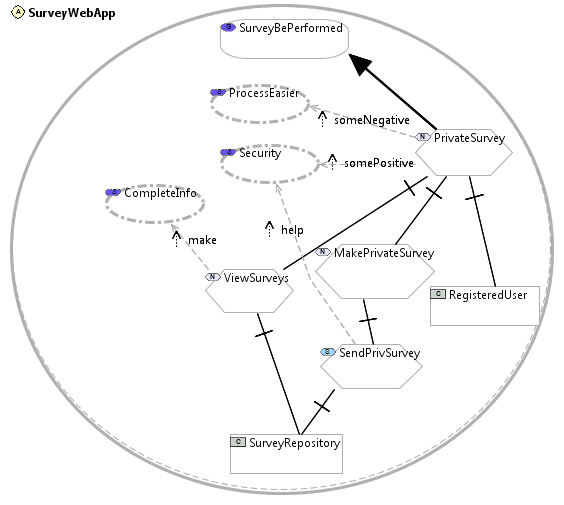
\includegraphics[width=0.8\textwidth]{img/EjemploICCSAReqFinales.png}
\end{center}
\caption{Los nuevos requisitos a implementar en el modelo de dominio.}
\label{fig:req2iccsa}
\end{figure}


\subsubsection{Optimizaci�n de Requisitos No-Funcionales en Aplicaciones Web}
\label{c1:optimizacion}

Como se ha motivado anteriormente, las aplicaciones Web tienen una audiencia amplia y heterog�nea \cite{aguilarDSDM, irene08}, debido a esto, el dise�ador se enfrenta a una problem�tica muy particular: �c�mo dise�ar la aplicaci�n optimizando el m�ximo n�mero posible de requisitos no-funcionales, de tal forma que la aplicaci�n Web sea capaz de satisfacer, en medida de lo posible, a la amplia y heterog�nea audiencia?, una opci�n consiste en enriquecer a las metodolog�as de dise�o para que sean capaces de asistir al dise�ador en la etapa de requisitos, es decir, que permitan seleccionar distintas opciones de dise�o en base a la audiencia de la aplicaci�n Web. 

Por lo tanto, en A-OOH se ha implementado el algoritmo Optimizaci�n de Pareto \cite{Pareto1} para proveer al dise�ador con un conjunto de alternativas de dise�o basadas en la prioridad de los requisitos no-funcionales. La Optimizaci�n de Pareto, llamada as� en honor de su introductor, Vilfredo Pareto, es un concepto de la econom�a con aplicaci�n tanto en esa disciplina como en ciencias sociales e ingenier�a \cite{KungPareto}. El concepto est� relacionado con estudios de eficiencia econ�mica y distribuci�n del ingreso y establece como eficiente aquella situaci�n en la cual se cumple que no es posible beneficiar a m�s individuos en un sistema sin perjudicar a otros. 

%Informaci�n m�s detallada sobre la implementaci�n del algoritmo se encuentra en el Cap�tulo \ref{c6} de la tesis doctoral.

La Optimizaci�n de Pareto ha sido ampliamente aplicada en la ingenier�a de \emph{software} \cite{Pareto3}, principalmente, en problemas en los que hay 2 o m�s objetivos, este tipo de problema es conocido como problema multi-objetivo (PMO) \cite{Pareto4}. En un problema de optimizaci�n, se trata de encontrar una soluci�n que represente el valor �ptimo para una funci�n objetivo \cite{Pareto5}.

Una caracter�stica de los PMO es que, como regla general, tienen un conjunto de soluciones, que inclusive puede ser infinito, y entonces los algoritmos deben describir lo mejor posible este conjunto. Por lo tanto, en este trabajo,  se han realizado algunas modificaciones que permiten obtener mejores representaciones de los conjuntos soluci�n. Informaci�n m�s detallada se encuentra en el Cap�tulo \ref{c6} de la tesis doctoral. 

Para un mejor entendimiento de la propuesta presentada en este apartado, se han adaptado una serie de definiciones para la aplicaci�n del algoritmo �ptimo de Pareto, estas son presentadas a continuaci�n:

\newtheorem{definicion}{\rule{0.2in}{0.11in} {\rm Ejemplo }}

\newtheorem{defi}{{\sc \textbf{Definici�n.}}} 

\begin{defi}\label{Def1}
\textbf{Optimizaci�n de Pareto:} dado un conjunto de ubicaciones alternativas y un conjunto de individuos, la ubicaci�n ``A'' es una optimizaci�n sobre la ubicaci�n ``B'' si solo si ``A'' puede al menos, optimizar a un individuo mejor que ``B'', sin deteriorar a otro individuo'' \emph{\cite{Pareto2, Pareto1}}.  
\end{defi}

En la Definici�n \ref{Def1}, las ubicaciones alternativas corresponden con el estado del requisito funcional, es decir, si el requisito est� o no est� implementado. Por otra parte, el conjunto de individuos comprende al conjunto de requisitos funcionales utilizados por el algoritmo. Mientras que, optimizar a un individuo mejor que ``B'', significa maximizar a los requisitos no-funcionales. Finalmente, en la Definici�n \ref{Def1} la frase ``\emph{sin deteriorar a otro individuo}'' se refiere a no afectar negativamente a los requisitos no-funcionales. 

\begin{defi}\label{Def2}
\textbf{Configuraci�n �ptima de Pareto:} es a aquella configuraci�n que mejor satisfaga a un requisito no-funcional mientras satisface a los dem�s de igual o mejor forma. 
\end{defi}

\begin{defi}\label{Def3}
\textbf{Configuraci�n:} una configuraci�n esta formada por un conjunto de requisitos funcionales que pueden ser implementados en los modelos conceptuales de la aplicaci�n Web.
\end{defi}

\begin{defi}\label{Def4}
\textbf{Frontera de Pareto:} es el espacio de soluci�n constituido por el conjunto de soluciones �ptimas de Pareto, es decir, las soluciones que no son dominadas por ninguna otra soluci�n.
\end{defi}

\begin{defi}\label{Def5}
\textbf{Dominio entre Soluciones:} se dice que una soluci�n no es dominada por otra soluci�n cuando, en el espacio de soluci�n, no existe ninguna otra que mejor satisfaga a un requisito no-funcional sin deteriorar a otro.
\end{defi}

El conjunto de soluciones �ptimas de Pareto puede ser utilizado por el dise�ador para la toma de decisiones, por ejemplo, cuando necesite seleccionar la configuraci�n que mejor balancee la compensaci�n entre los requisitos no-funcionales y cuando necesite considerar la maximizaci�n sobre un requisito no-funcional en particular.

\begin{figure}
\begin{center}
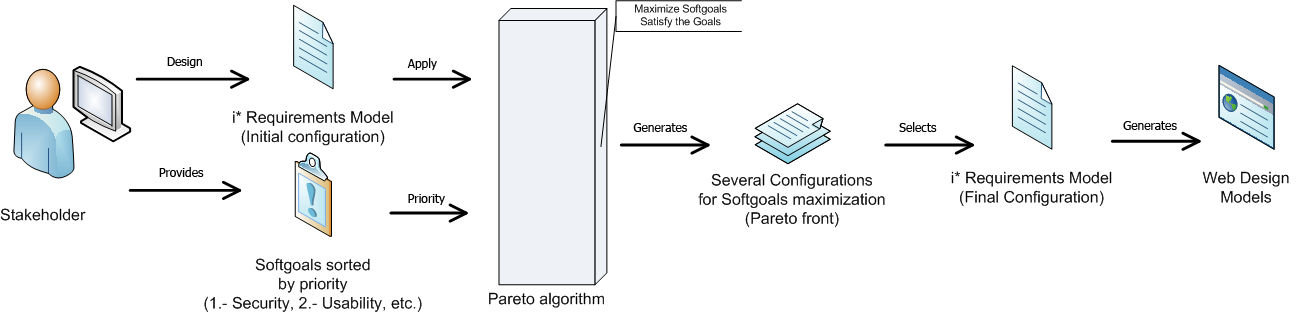
\includegraphics[width=\textwidth]{img/ParetoApproach.png}
\end{center}
\caption{Propuesta para la optimizaci�n de requisitos no-funcioales en aplicaciones Web.}
\label{fig:ParetoApproach}
\end{figure}

La Figura \ref{fig:ParetoApproach} muestra los pasos definidos en la propuesta descrita en este apartado para la optimizaci�n de requisitos no-funcionales. En el primer paso, el \emph{stakeholder}, concretamente en el rol de dise�ador, especificar� los requisitos de la aplicaci�n Web utilizando el marco de modelado orientado a objetivos \emph{i*}, as� mismo, establecer� una lista de requisitos no-funcionales a priorizar. El segundo paso consiste en aplicar el algoritmo Optimizaci�n de Pareto, como resultado del algoritmo se obtendr� un conjunto de configuraciones. Finalmente, ln �ltimo paso consiste en la selecci�n de la configuraci�n que mejor satisfaga la lista de requisitos no-funcionales a priorizar. Es importante destacar que los requisitos no-funcionales son considerados \emph{Softgoals} en la propuesta para la especificaci�n de requisitos, como se defini� en la Secci�n \ref{especificacion}.

A continuaci�n, se presenta un ejemplo conciso para ejemplificar paso a paso la aplicaci�n de la propuesta para la optimizaci�n de requisitos \emph{Softgoals} en aplicaciones Web. El caso de estudio es acerca de una aplicaci�n Web para la gesti�n de conferencias (\emph{Conference Management System})\footnote{La especificaci�n completa del caso de estudio se encuentra en \url{http://users.dsic.upv.es/~west/iwwost01}}. El prop�sito de la aplicaci�n Web es brindar soporte al proceso de env�o, evaluaci�n y selecci�n de los art�culos para una conferencia. La Figura \ref{fig:CasoEstudioWISM}, muestra la especificaci�n de requisitos de la aplicaci�n Web (modelo de requisitos \emph{i*}). El objetivo de la aplicaci�n Web consiste en ``\emph{Process of review of papers be selected}'', para satisfacer el objetivo, es necesario la implementaci�n de alguno de los requisitos navegacionales ``\emph{Blind review process}'' y ``\emph{Normal review process}''. En este ejemplo el objetivo es logrado a trav�s del requisito navegacional ``\emph{Blind review process}''. Para una explicaci�n detallada del ejemplo se recomienda al lector consultar el Cap�tulo \ref{c6} de la tesis doctoral.

En la especificaci�n de requisitos, tambi�n se puede observar que algunos requisitos necesitan de otros para poder cumplir con su funci�n, tal es el caso del requisito navegacional ``\emph{Review paper}'' el cual necesita del requisito de servicio ``\emph{Submit review}''. Adem�s, algunos requisitos afectan de forma positiva o negativa a algunas \emph{Softgoals}, por ejemplo, el requisito de servicio ``\emph{Download paper without author's name}'' afecta de forma positiva a la \emph{Softgoal} ``\emph{Privacy be maximized}'' y de forma negativa a ``\emph{Obtain more complete info}''. Las contribuciones de los requisitos funcionales a las \emph{Softgoals} pueden verse en la Tabla \ref{tab:contribuciones}.

\begin{figure}
\begin{center}
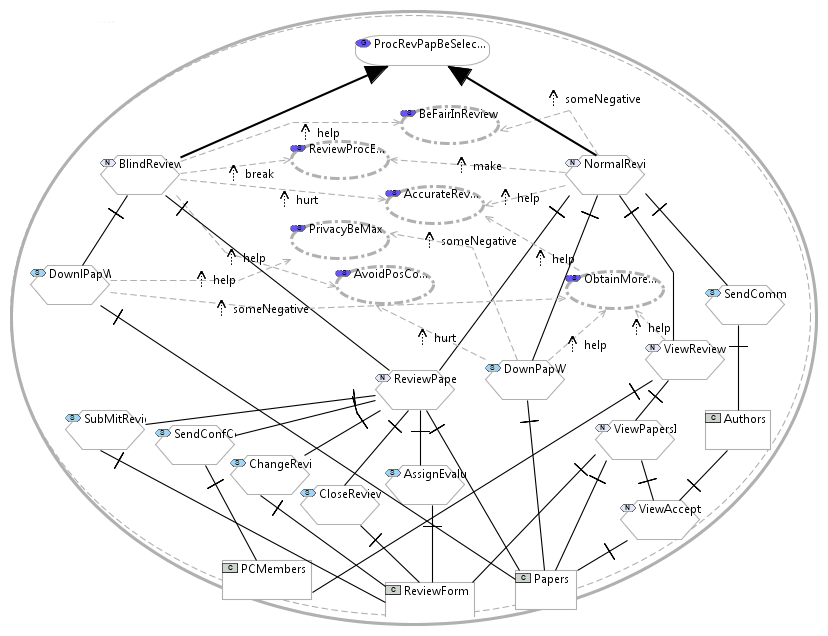
\includegraphics[width=\textwidth]{img/CasoEstudioWISM.png}
\end{center}
\caption{Especificaci�n de requisitos de la aplicaci�n Web para la gesti�n de conferencias.}
\label{fig:CasoEstudioWISM}
\end{figure}

\begin{table}
 \centering
 \small
 \caption{Tipos de contribuciones.}\label{tab:contribuciones}
\begin{tabular}{|l | c |}
\hline
\textbf{Contribuci�n} & \textbf{Tipo de Contribuci�n} \\
\hline
Positiva& Help \\
Positiva de fuerza desconocida & Some + \\
Negativa & Hurt \\
Negativa de fuerza desconocida & Some - \\
Negativa suficiente para no satisfacer una \emph{Softgoal}& Break \\
Positiva suficiente para satisfacer una \emph{Softgoal} & Make \\
\hline
\end{tabular}
\end{table}

Una vez especificados los requisitos de la aplicaci�n Web, es necesario elaborar una lista que contenga a los requisitos (implementados o no) que realicen alg�n tipo de contribuci�n a alguna \emph{Softgoal}. La Tabla \ref{tab:listaElementosIntencionales}, muestra una lista de requisitos y el tipo de contribuci�n (Tabla \ref{tab:contribuciones}) hacia las \emph{Softgoals}, en donde: S1 se refiere a la \emph{Softgoal} \emph{``Be fair in review''}, la \emph{Softgoal} representa en el modelo de requisitos que el proceso de revisi�n en la aplicaci�n para la gesti�n de conferencias debe de ser imparcial, la \emph{Softgoal} S2 corresponde a \emph{``Review process easier''} y se refiere a que el proceso de revisi�n debe de ser lo m�s simple posible de realizar gracias a que se llevar� a cabo por medio de la aplicaci�n Web, la \emph{Softgoal} S3 llamada \emph{``Accurate review process''} es utilizada para indicar que el proceso de revisi�n debe de ser lo m�s preciso posible, S4 se refiere a la \emph{Softgoal} \emph{``Privacy be maximized''} para indicar que en la aplicaci�n Web la seguridad debe de ser maximizada cuando se realicen ciertos requisitos funcionales en particular, la \emph{Softgoal} S5 nombrada \emph{``Avoid possible conflicts of interest''}, permite representar la �tica del usuario de la aplicaci�n Web debido a que este deber� ser capaz de evitar conflictos de inter�s al momento de realizar la revisi�n del art�culo asignado y la \emph{Softgoal} S6, \emph{``Obtain more complete info''} la cual representa que al realizarse un proceso de revisi�n normal, el usuario de la apliaci�n obtendr� informaci�n m�s detallada sobre los autores del art�culo que le ha sido asignado.

\begin{table}
 \centering
\small %\addtolength{\tabcolsep}{-5pt}
 \caption{Las contribuciones de los requisitos hacia las \emph{Softgoals}.}\label{tab:listaElementosIntencionales}
\begin{tabular}{| l | c| c | c | c | c | c |}
\hline
\textbf{Requisitos} &
\textbf{\emph{``S1''}} &
\textbf{\emph{``S2''}} &
\textbf{\emph{``S3''}} &
\textbf{\emph{``S4''}} &
\textbf{\emph{``S5''}} &
\textbf{\emph{``S6''}}
\\
\hline
  \emph{``Blind review process''} & Help & Break & Hurt & Help & - & -\\
  \textbf{\emph{``Download papers without authors' name''}} & \textbf{-} & \textbf{-} & \textbf{-} & \textbf{-} & \textbf{Help} & \textbf{Some -}\\
  \emph{``Normal review process''} & Some - & Make & Help & - & - & -\\
  \emph{``Download paper with author's name''} & - & - & - & Hurt & Some - & Help\\
  \emph{``View review process status''} & - & - & - & - & - & Help\\
\hline
\end{tabular}
\end{table}

A continuaci�n, es necesario almacenar cada configuraci�n posible de los requisitos listados en la Tabla \ref{tab:listaElementosIntencionales}, en donde: la variable ``I'' representa el estado ``implementado'' y la variable ``N'' el estado ``no implementado''. Por lo tanto, tenemos 32 posibles configuraciones (Tabla \ref{tab:front}, columnas 1 y 2).

Adem�s, es necesario asignar un peso a cada tipo de contribuci�n, para esto, deben de asignarse por cada tipo el peso(W):  w= +1 si el tipo de contribuci�n es  ``\emph{Help}'',  w= -1 si es ``\emph{Hurt}'', w= +2 para el tipo ``\emph{Some +}'' , w= -2 para ``\emph{Some -}'', w= +4 si es del tipo ``\emph{Make}'' y w= -4 para el tipo ``\emph{Break}''. 

Es importante mencionar que el valor del umbral de la contribuci�n depende de los fundamentos del marco de modelado \emph{i*}, por ejemplo, teniendo en cuenta que la contribuci�n del tipo ``\emph{Make}'' es el valor positivo m�s fuerte que sirve para al satisfacci�n de una \emph{Goal} o \emph{Softgoal}, se decidi� asignarle el valor num�rico 4. Esta forma de proceder contin�a en proceso de estudio con la idea de tener una distribuci�n de los valores num�ricos lo m�s confiable posible, por esta raz�n se est�n realizando una serie de experimentos actualmente.

%Por ejemplo, dada la matriz (\ref{mt:matriz}), tenemos que, para la fila 3 (requisito ``\emph{Normal review process}'') y columna 2 (\emph{Softgoal ``Review process easier''}) la matriz muestra '+4', es decir una contribuci�n del tipo ``\emph{Make}'' si el requisito es implementado.

\begin{equation}
\small
M= 
\begin{pmatrix}
  \hfill {\color {black} +1} & \hfill {\color {red} -4} & \hfill{\color {red} -1} & {\color {black} 0} & \hfill {\color {black} +1} & {\color {black} 0}\\
  {\color {black} 0} & {\color {black} 0} & {\color {black} 0} & \hfill {\color {black} +1} & {\color {black} 0} & \hfill{\color {red} -2} \\
  \hfill{\color {red} -2} & \hfill {\color {black} +4} & \hfill {\color {black} +1} & {\color {black} 0} & {\color {black} 0} & {\color {black} 0} \\
  {\color {black} 0} & {\color {black} 0} & {\color {black} 0} & \hfill{\color {red} -2} & \hfill{\color {red} -1} & \hfill {\color {black} +1}\\
  {\color {black} 0} & {\color {black} 0} & {\color {black} 0} & {\color {black} 0} & {\color {black} 0} & \hfill {\color {black} +1} \\
\label{mt:matriz}
\end{pmatrix}
\end{equation}

Con los pesos establecidos, el siguiente paso consiste en crear una matriz para calcular los valores n�mericos asociados cada configuraci�n (Tabla \ref{tab:front}, columnas 7 a 12), por ejemplo para la configuraci�n X25, si el requisito R1 \emph{``Blind review process''} no es implementado, tenemos que la \emph{Softgoal} \emph{``Be fair in review''} ser� afectada (-2). Por �ltimo, se calcula si la configuraci�n es Frontera de Pareto (Tabla \ref{tab:front}, columnas 13), para hacerlo, se deben comparar cada una de las configuraciones indicando si es que existe una que sea mejor que otra, por ejemplo, la configuraci�n X3 est� en la Frontera de Pareto por que es mejor que las configuraciones X1 y X2 debido a que maximiza al menos a un individuo, es decir, maximiza a la \emph{Softgoal} 5 \emph{``Avoid possible conflicts of interest''}.


\begin{table}[!ht]
 \centering
\small%\tiny %\addtolength{\tabcolsep}{-5pt}
 \caption{The posible requirements to implement or not for the softgoal tradeoff.}\label{tab:front}
\begin{tabular}{|c|c|c|c|c|c|c|c|c|c|c|c|c|c|}
\hline
\textbf{Configuraci�n} & \textbf{R1} & \textbf{R2} & \textbf{R3} & \textbf{R4} & \textbf{R5} & \textbf{F(S1)} & \textbf{F(S2)} & \textbf{F(S3)} & \textbf{F(S4)} & \textbf{F(S5)} & \textbf{F(S6)} & \textbf{Pareto front}
\\
\hline
\textbf{X1} & I & I & I & I & I & -1 & 0 & 0 & -1 & 0 & 0 & No\\ %\rowcolor[rgb]{0.8,0.8,0.8}
\textbf{X2} & I & I & I & I & N & -1 & 0 & 0 & -1 & 0 & -1 & No\\
\rowcolor[rgb]{0.8,0.8,0.8} \textbf{X3} & I & I & I & N & I & -1 & 0 & 0 & 1 & 1 & -1 & Yes\\
\textbf{X4} & I & I & I & N & N & -1 & 0 & 0 & 1 & 1 & -2 & No\\
\rowcolor[rgb]{0.8,0.8,0.8} \textbf{X5} & I & I & N & I & I & 1 & -4 & -1 & -1 & 0 & 0 & Yes\\
\textbf{X6} & I & I & N & I & N & 1 & -4 & -1 & -1 & 0 & -1 & No\\
\rowcolor[rgb]{0.8,0.8,0.8} \textbf{X7} & I & I & N & N & I & 1 & -4 & -1 & 1 & 1 & -1 & Yes\\
\textbf{X8} & I & I & N & N & N & 1 & -4 & -1 & 1 & 1 & -2 & No\\
\rowcolor[rgb]{0.8,0.8,0.8} \textbf{X9} & I & N & I & I & I & -1 & 0 & 0 & -2 & 0 & 2 & Yes\\
\textbf{X10} & I & N & I & I & N & -1 & 0 & 0 & -2 & 0 & 1 & No\\
\rowcolor[rgb]{0.8,0.8,0.8} \textbf{X11} & I & N & I & N & I & -1 & 0 & 0 & 0 & 1 & 1 & Yes\\
\textbf{X12} & I & N & I & N & N & -1 & 0 & 0 & 0 & 1 & 0 & No\\
\rowcolor[rgb]{0.8,0.8,0.8} \textbf{X13} & I & N & N & I & I & 1 & -4 & -1 & -2 & 0 & 2 & Yes\\
\textbf{X14} & I & N & N & I & N & 1 & -4 & -1 & -2 & 0 & 1 & No\\
\rowcolor[rgb]{0.8,0.8,0.8} \textbf{X15} & I & N & N & N & I & 1 & -4 & -1 & 0 & 1 & 1 & Yes\\
\textbf{X16} & I & N & N & N & N & 1 & -4 & -1 & 0 & 1 & 0 & No\\
\rowcolor[rgb]{0.8,0.8,0.8} \textbf{X17} & N & I & I & I & I & -2 & 4 & 1 & -1 & -1 & 0 & Yes\\
\textbf{X18} & N & I & I & I & N & -2 & 4 & 1 & -1 & -1 & -1 & No\\
\rowcolor[rgb]{0.8,0.8,0.8} \textbf{X19} & N & I & I & N & I & -2 & 4 & 1 & 1 & 0 & -1 & Yes\\
\textbf{X20} & N & I & I & N & N & -2 & 4 & 1 & 1 & 0 & -2 & No\\
\textbf{X21} & N & I & N & I & I & 0 & 0 & 0 & -1 & -1 & 0 & No\\
\textbf{X22} & N & I & N & I & N & 0 & 0 & 0 & -1 & -1 & -1 & No\\
\rowcolor[rgb]{0.8,0.8,0.8} \textbf{X23} & N & I & N & N & I & 0 & 0 & 0 & 1 & 0 & -1 & Yes\\
\textbf{X24} & N & I & N & N & N & 0 & 0 & 0 & 1 & 0 & -2 & No\\
\rowcolor[rgb]{0.8,0.8,0.8} \textbf{X25} & N & N & I & I & I & -2 & 4 & 1 & -2 & -1 & 2 & Yes\\
\textbf{X26} & N & N & I & I & N & -2 & 4 & 1 & -2 & -1 & 1 & No\\
\rowcolor[rgb]{0.8,0.8,0.8} \textbf{X27} & N & N & I & N & I & -2 & 4 & 1 & 0 & 0 & 1 & Yes\\
\textbf{X28} & N & N & I & N & N & -2 & 4 & 1 & 0 & 0 & 0 & No\\
\rowcolor[rgb]{0.8,0.8,0.8} \textbf{X29} & N & N & N & I & I & 0 & 0 & 0 & -2 & -1 & 2 & Yes\\
\textbf{X30} & N & N & N & I & N & 0 & 0 & 0 & -2 & -1 & 1 & No\\
\rowcolor[rgb]{0.8,0.8,0.8} \textbf{X31} & N & N & N & N & I & 0 & 0 & 0 & 0 & 0 & 1 & Yes\\
\textbf{X32} & N & N & N & N & N & 0 & 0 & 0 & 0 & 0 & 0 &  No\\
\hline
\end{tabular}
\end{table}

Finalmente, el �ltimo paso consiste, aparte de maximizar las \emph{Softgoals}, continuar cumpliendo con el objetivo establecido en el modelo de requisitos (\emph{``Process of review papers be selected''}). Para esto, es necesario crear una lista de \emph{Softgoals} ordenadas por prioridad (Tabla \ref{tab:prioridad}). En base a la lista, se debe de seleccionar de la Tabla \ref{tab:front} las configuraciones que adem�s de estar en la Frontera de Pareto cumplen con el objetivo, y de esta forma escoger la configuraci�n que maximice las \emph{Softgoals}.

\begin{table}[!ht]
 \centering
\small%\tiny %\addtolength{\tabcolsep}{-5pt}
 \caption{Lista de \emph{Softgoals}.}\label{tab:prioridad}
\begin{tabular}{| c | c|}
\hline
\textbf{Prioridad} & \textbf{Softgoal}
\\
\hline
\textbf{1} & \emph{``S4.- Privacy be maximized''}  \\
\textbf{2} & \emph{``S2.- Review process easier''} \\
\textbf{3} & \emph{``S3.- Accurate review process''} \\
\textbf{4} & \emph{``S1.- Be fair in review''} \\
\textbf{5} & \emph{``S5.- Avoid possible conflicts os interest''}\\
\textbf{6} & \emph{``S6.- Obtain more complete info''}  \\
\hline
\end{tabular}
\end{table}

Para este ejemplo, ``X3'', ``X7'' y ``X17'' cumplen con el objetivo, de las tres configuraciones, la configuraci�n X3 es la mejor opci�n, porque de acuerdo con la lista (Tabla \ref{tab:prioridad}), ``S4'' y ``S2'' son las \emph{Softgoals} a priorizar, por tanto, la configuraci�n ``X17'' maximiza ``S2'', sin embargo afecta negativamente a la \emph{Softgoal} 4 (Tabla \ref{tab:front}). En cambio, la configuraci�n ``X3'' maximiza a la \emph{Softgoal} ``S4'' (1) y no afecta a la \emph{Softgoal} ``S2'' (0).

\section{Hacia la Gesti�n de Requisitos en las \emph{Rich Internet Applications}}
\label{c1:rias}

En la actualidad, las aplicaciones Web evolucionan constantemente, por ejemplo, se evolucion� de las p�ginas HTML\footnote{\emph{Hyper Text Markup Language}} est�ticas al siguiente nivel en donde la mayor parte del contenido era generado din�micamente a trav�s de diversos sistemas y bases de datos. Conforme a esta evoluci�n, se crearon las primeras metodolog�as para el desarrollo de aplicaciones Web, como OOHDM \cite{OOHDM1995}. Al continuar la evoluci�n natural de las aplicaciones Web, se tomaron en cuenta factores importantes como la est�tica, el contenido, la funcionalidad y la personalizaci�n en las metodolog�as de desarrollo (UWE \cite{Koch02}, WebML \cite{WebML}, NDT \cite{NDT}, OOWS \cite{OOWS2001}, A-OOH  \cite{irene08}). 

Recientemente, las aplicaciones Web han experimentado cambios significativos relacionados con la tecnolog�a de implementaci�n, la distribuci�n de la l�gica de negocio entre el cliente y el servidor, la comunicaci�n que se establece entre ambos as� como las interfaces de usuario (UIs). Este tipo de aplicaciones Web recibe el nombre de RIAs (\emph{Rich Internet Applications}) y se caracterizan por ofrecer al usuario una serie de caracter�sticas muy similares a las de las aplicaciones de escritorio, as� como la inclusi�n de contenido multimedia bajo demanda, la actualizaci�n de contenido din�micamente, es decir, sin que la p�gina Web vuelva a ser generada por completo tras una petici�n del usuario y la posibilidad de comunicaci�n por medio del audio y video.  La Figura  \ref{fig:RiasDiagramaVenn}\footnote{Imagen tomada de \url{http://www.simonwhatley.co.uk/rich-internet-applications-a-background}} muestra un diagrama de Venn en donde se representa la combinaci�n de tecnolog�as que han dado origen a las RIAs, por tanto se puede deducir f�cilmente que las RIAs son una combinaci�n de la tecnolog�a y/o funcionalidad de las aplicaciones de escritorio, de las aplicaciones Web y de las tecnolog�as de comunicaci�n (audio, video, Internet).


\begin{figure}
\begin{center}
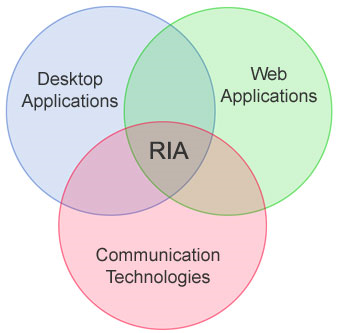
\includegraphics[width=0.4\textwidth]{img/RiasDiagramaVenn.png}
\end{center}
\caption{Diagrama de Venn que ejemplifica las caracter�sticas de las RIAs.}
\label{fig:RiasDiagramaVenn}
\end{figure}


Sin embargo, la evoluci�n de las aplicaciones Web a RIAs conlleva a una mayor complejidad en su desarrollo debido al nivel de funcionalidad e interactividad que ofrecen al usuario. Por lo tanto, son m�s dif�ciles de dise�ar e implementar que las aplicaciones Web 1.0. Por esta raz�n, las metodolog�as para el desarrollo de aplicaciones Web han sido objeto de mejoras (adaptaciones en algunos casos) y han surgido nuevas aproximaciones espec�ficamente para el desarrollo de RIAs \cite{Preciado}. Dentro del grupo de aproximaciones que han sido extendidas para el soporte de RIAs encontramos a OOHDM \cite{OOHDMRIA}, OOH con la extenci�n OOH4RIAs \cite{OOH4RIAMethod}, UWE con las extensiones UWE-Patterns \cite{UWEpatterns4RIA}, UWE-R \cite{UWER} y UWE-RUX \cite{RUXMethod}, WebML \cite{Bozzon2008, Bozzon2006} y OOWS  \cite{Valverde2010}. Por otra parte, dentro del grupo de aproximaciones creadas exclusivamente para el desarrollo de RIAS encontramos a RUX-Model \cite{Preciado2008}, \emph{Internet Aplication Modeling Language} \cite{IAML} y ADRIA \cite{ADRIA2,ADRIA1}, para informaci�n m�s detallada sobre las aproximaciones tradicionales y las de nueva creaci�n el lector puede consultar el Ap�ndice \ref{a2}. La idea principal de las aproximaciones es brindar soporte a las caracter�sticas particulares de las RIAs, pero la mayor�a de las metodolog�as se han enfocado principalmente en cuestiones de presentaci�n \cite{RUXMethod, Preciado2007} y en capacidades de interacci�n \cite{OOH4RIAMethod} descuidando la etapa de an�lisis y especificaci�n de requisitos. Esto es una desventaja muy importante a considerar, debido a que el dise�ador tiene que lidiar con los requisitos de la Web 1.0, como lo es la navegaci�n m�s los requisitos espec�ficos de las RIAs, tales como, la capacidad de respuesta o la reducci�n del ancho de banda \cite{ReqForRIA}. 

Adem�s, el dise�ador debe de considerar la distribuci�n de los requisitos funcionales, es decir, si son implementados en el cliente o en el servidor y como es que la distribuci�n afecta el cumplimiento de las \emph{Softgoals}. Por ejemplo, si se analiza la distribuci�n de los requisitos funcionales entre el cliente y el servidor, se podr�n tomar decisiones de dise�o que favorezcan la reducci�n de la cantidad y frecuencia del tr�fico entre el cliente y el servidor, lo que sin duda alguna resulta en un beneficio para la seguridad de la RIA. Por lo tanto, elegir d�nde ser�n implementados los requisitos funcionales (cliente o servidor) es una decisi�n fundamental (m�s no trivial) para el correcto desempe�o de la RIA.

En esta secci�n, se presenta una adaptaci�n del trabajo presentado en la secci�n \ref{c1:optimizacion} (el trabajo se explica en detalle en el Cap�tulo \ref{c6} de la tesis) para asistir al dise�ador al momento de decidir sobre la distribuci�n de los requisitos funcionales de la aplicaci�n Web entre el cliente y el servidor. Para esto, se han definido una serie de pasos los cuales pueden verse en la Figura \ref{fig:overview}. El primer paso consiste en la especificaci�n de los requisitos por parte del dise�ador y existen dos formas para llevarla a cabo, en la primera, el dise�ador puede crear un modelo de requisitos RIA a partir de un modelo de requisitos para aplicaciones Web 1.0, la forma de hacerlo es especificar en el modelo de requisitos los requisitos particulares de las RIAs; la segunda forma, consiste en crear un modelo de requisitos desde cero, es decir, exclusivamente con los requisitos de las RIAs. El segundo paso es aplicar el algoritmo de �ptimo de Pareto para obtener el conjunto de configuraciones Cliente/Servidor. Por �ltimo, en el tercer paso el dise�ador solo tendr� que seleccionar el modelo de requisitos final con el cu�l podr� saber qu� requisitos funcionales implementar en el servidor o en el cliente considerando la optimizaci�n de las \emph{Softgoals}. Para obtener informaci�n m�s detallada sobre la adaptaci�n de la propuesta presentada en el Cap�tulo \ref{c6}, as� como las definiciones y conceptos de esta secci�n consultar Ap�ndice \ref{a2} y Ap�ndice \ref{a3}.

A continuaci�n, se presenta un caso de estudio para ejemplificar la propuesta presentada en este apartado de la tesis doctoral. El caso de estudio es acerca de una compa��a de bioinform�tica, la cual tiene como objetivo ofrecer servicios en l�nea sobre el an�lisis del gen�ma humano. La aplicaci�n Web permitir� al usuario subir la informaci�n sobre un gen, analizar la informaci�n y obtener reportes personalizados. El primer y �nico servicio disponible para el usuario ser� el reporte de enfermedades al que es vunerable el gen, para lograrlo, se comparar� la informaci�n proporcionada por el usuario con la base de datos de genes de la compa��a. La compa��a, desea ofrecer una Web basada en RIA con la finalidad de ofrecer una aplicaci�n Web lo suficientemente atractiva e interactiva para los usuarios. Para esto, el equipo de desarrollo de la compa��a quiere estudiar y analizar los beneficios que se obtendr�n de la distribuci�n de los requisitos funcionales entre el servidor y el cliente, as� como el impacto que tendr�n en las \emph{Softgoals} para poder considerar asuntos relacionados a la seguridad de la informaci�n proporcionada por el usuario as� como estudiar la compatibilidad cuando sea mostrada la informaci�n a los usuarions de la RIA. Para efectos demostrativos, en el caso de estudio nos enfocaremos en los requisitos necesarios para el reporte de enfermedades.

\begin{figure}
\begin{center}
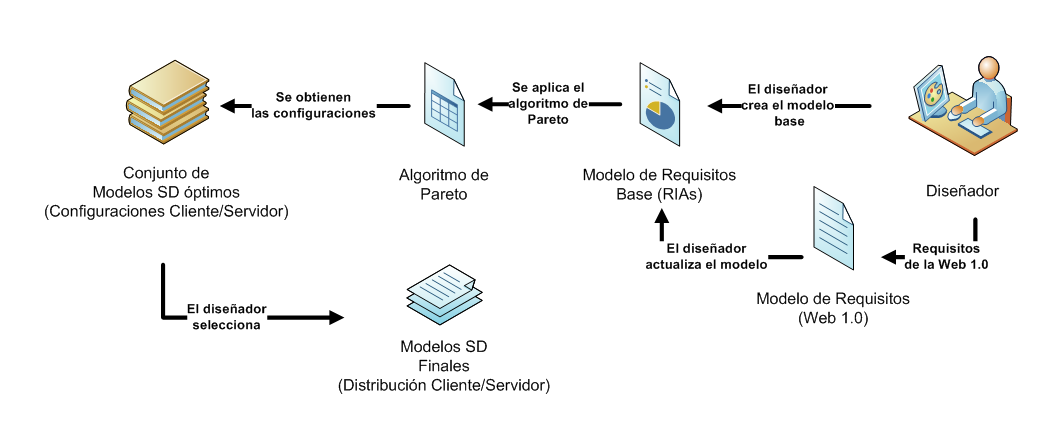
\includegraphics[width=\textwidth]{img/OverviewRIAs.png}
\end{center}
\caption{Visi�n general de la propuesta para el an�lisis de requisitos RIA.} \label{fig:overview}
\end{figure}


El primer paso consiste en la especificaci�n del modelo de requisitos base para RIAs por parte del dise�ador. En �l, el dise�ador deber� especificar los objetivos, los requisitos funcionales y las \emph{Softgoals} necesarias para modelar el reporte de enfermedades (Figura \ref{fig:baseRIA}).

\begin{figure}
\begin{center}
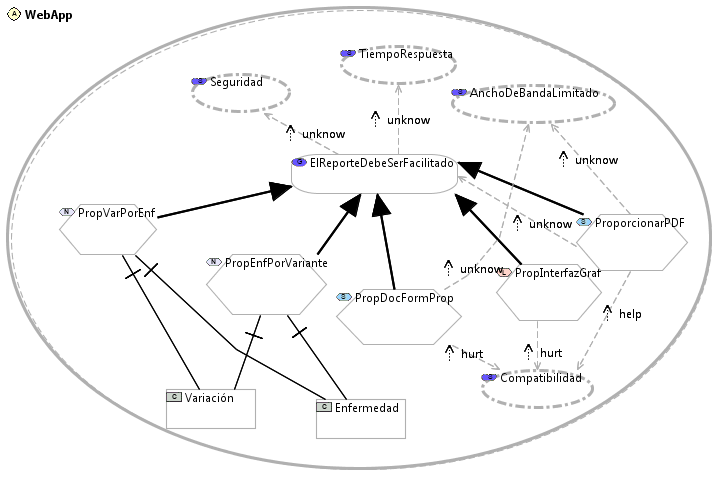
\includegraphics[width=\textwidth]{img/EjemploRIAs.png}
\end{center}
\caption{Modelo de requisitos RIA base.} \label{fig:baseRIA}
\end{figure}

Debido a que a�n no sabemos qu� requisitos ser�n ubicados de lado del cliente o de lado del servidor, las contribuciones por parte de los requisitos a las \emph{Softgoals} son etiquetadas como ``\emph{unknown}''. En el particular caso de la \emph{Softgoal} ``Compatibilidad'', las contribuciones recibidas por parte de los requisitos quedan establecidas en este paso debido a que no dependen del lugar donde se implementar� el requisito (cliente o servidor). Las contribuciones originadas en el requisito ``Proporcionar interfaz gr�fica'' tambi�n son etiquetadas debido a que el requisito solo puede ser implementado del lado del cliente.

El segundo paso consiste en aplicar el algoritmo �ptimo de Pareto (Figura \ref{fig:overview}) para obtener el conjunto de configuraciones Cliente/Servidor. Para poder hacerlo, es necesario identificar a los requisitos que realizan contribuciones a las \emph{Softgoals}, no se deber� considerar el requisito ``Proporcionar interfaz gr�fica'' por que, como lo mencionamos antes, solo es posible implementarlo del lado del cliente. La Tabla \ref{tab:softgoals-req} muestra los requisitos y \emph{Softgoals} a utilizar.

\begin{table}
 \centering
 \caption{\emph{Softgoals} y Requisitos detectados en el modelo de requisitos RIA base.}\label{tab:softgoals-req}
\begin{tabular}{|l | l |}
\hline
\textbf{\emph{Softgoals}} & \textbf{Requisitos} \\
\hline
S1.- Seguridad & R1.- Proporcionar variaciones por enfermedad \\
S2.- Tiempo de respuesta & R2.- Proporcionar enfermedad por variante \\
S3.- Compatibilidad & R3.- Proporcionar PDF \\
S4.- Ancho de banda limitado & R4.- Proporcionar documento en formato propietario \\
\hline
\end{tabular}
\end{table}

En seguida, es necesario calcular todas las posibles configuraciones Cliente/Servidor, en donde C representa si el requisito se implementar� en el Cliente y S si se implementar� en el Servidor, como puede verse en la Tabla \ref{tab:front}, de la columna 2 a la columna 5. Posteriormente, se deber�n obtener dos matrices (Matriz Cliente (\ref{mt:matriz}) y Matriz Servidor (\ref{mt:matrizServidor})) las cuales representan la contribuci�n de cada requisito a cada una de las \emph{softgoals}, por ejemplo, la fila 3 (requisito ``Proporcionar PDF''), columna 4 (\emph{softgoal} ``Tiempo de respuesta'') muestra +1 en la Matriz Cliente, por lo que es una contribuci�n del tipo ``\emph{Help}'' si el requisito es implementado en el Cliente, en cambio, en la Matriz Servidor muestra -1, indicando una contribuci�n del tipo ``\emph{Hurt}'' si el requisito se implementa en el Servidor. Con las matrices se calcular� el resultado de las contribuciones de los requisitos a las \emph{Softgoals}, el cual es mostrado de la columna 6 a la columna 9 de la Tabla \ref{tab:front}. Por �ltimo, se indica si la configuraci�n est� o no en la Frontera de Pareto (�ltima columna).

\begin{equation}
%\tiny
M_{i_j}^k = 
\begin{pmatrix}
  \hfill {\color {red} -1} & \hfill {\color {black} +1} & \hfill{\color {black} 0} & {\color {black} 0} \\
  \hfill {\color {red} -1} & \hfill {\color {black} +1} & \hfill{\color {black} 0} & {\color {black} 0} \\
  \hfill {\color {red} -1} & \hfill {\color {black} +1} & \hfill{\color {black} +1} & {\color {red} -1} \\
  \hfill {\color {red} -1} & \hfill {\color {black} +1} & \hfill{\color {red} -1} & {\color {red} -1} \\
\label{mt:matriz}
\end{pmatrix}
\end{equation}

\begin{equation}
%\tiny
M_{i_j}^k = 
\begin{pmatrix}
  \hfill {\color {black} +1} & \hfill {\color {red} -1} & \hfill{\color {black} 0} & {\color {black} 0} \\
  \hfill {\color {black} +1} & \hfill {\color {red} -1} & \hfill{\color {black} 0} & {\color {black} 0} \\
  \hfill {\color {black} +1} & \hfill {\color {red} -1} & \hfill{\color {black} +1} & {\color {black} +1} \\
  \hfill {\color {black} +1} & \hfill {\color {red} -1} & \hfill{\color {red} -1} & {\color {black} +1} \\
\label{mt:matrizServidor}
\end{pmatrix}
\end{equation}
En la Tabla \ref{tab:front}, las filas de color gris son la Frontera de Pareto. Finalmente, en el tercer paso (ver Figura \ref{fig:overview}), el dise�ador puede seleccionar de la Frontera de Pareto la configuraci�n que mejor satisfaga las necesidades del \emph{stakeholder}, es decir, considerando a las \emph{Softgoals} de mayor inter�s. Por mencionar un ejemplo, tenemos que la configuraci�n X1 (Tabla \ref{tab:front}) es la mejor opci�n si la \emph{Softgoal} ``Tiempo de respuesta'' es la prioridad, en la soluci�n cada requisito ser� implementado de lado del Cliente y, de acuerdo con el resultado positivo de la columna 10 ($\Sigma$), las \emph{Softgoals} restantes ser�n maximizadas o permanecer�n igual, es decir, no ser�n afectadas negativamente. Por otro lado, la mejor opci�n respecto a la \emph{softgoal} ``Seguridad'' es la configuraci�n X16 (Figura \ref{fig:X16}), de acuerdo con $\Sigma$ (-2), mejorar la seguridad afectar� negativamente en algunas de las \emph{Softgoals}. 



\begin{table}
\centering
%\tiny%\addtolength{\tabcolsep}{-5pt}
 \caption{La posible distribuci�n de los requisitos entre el servidor y el cliente a trav�s de la compensaci�n de las \emph{softgoals}.}\label{tab:front}
    \begin{tabular}{|c|cccc|cccc|c|c|}
        \hline
        \textbf{Configuraci�n}          & \textbf{R1} & \textbf{R2} & \textbf{R3} & \textbf{R4} & \textbf{F(S1)} & \textbf{F(S2)} & \textbf{F(S3)} & \textbf{F(S4)} & \textbf{$\Sigma$} & \textbf{Frontera de Pareto} \\ \hline 
        \rowcolor[rgb]{0.8,0.8,0.8}X1  & C          & C          & C          & C          & -4            & +4            & 0             & +2            & +2               & Si                         \\ \hline
        X2                             & C          & C          & C          & S          & -2            & +2            & 0             & 0             & 0                & No debido a X5             \\ \hline
        X3                             & C          & C          & S          & C          & -2            & +2            & 0             & 0             & 0                & No debido a X6             \\ \hline
        X4                             & C          & C          & S          & S          & 0             & 0             & 0             & -2            & -2               & No debido a X13            \\ \hline
        \rowcolor[rgb]{0.8,0.8,0.8}X5  & C          & S          & C          & C          & -2            & +2            & 0             & +2            & +2               & Si                         \\ \hline
        \rowcolor[rgb]{0.8,0.8,0.8}X6  & C          & S          & C          & S          & 0             & 0             & 0             & 0             & 0                & Si                         \\ \hline
        \rowcolor[rgb]{0.9,0.9,0.9}X7  & C          & S          & S          & C          & 0             & 0             & 0             & 0             & 0                & Si (como X6)               \\ \hline
        X8                             & C          & S          & S          & S          & +2            & -2            & 0             & -2            & -2               & No debido a X14            \\ \hline
        \rowcolor[rgb]{0.9,0.9,0.9}X9  & S          & C          & C          & C          & -2            & +2            & 0             & +2            & +2               & Si (como X5)               \\ \hline
        \rowcolor[rgb]{0.9,0.9,0.9}X10 & S          & C          & C          & S          & 0             & 0             & 0             & 0             & 0                & Si (como X6)               \\ \hline
        \rowcolor[rgb]{0.9,0.9,0.9}X11 & S          & C          & S          & C          & 0             & 0             & 0             & 0             & 0                & Si (como X6)               \\ \hline
        X12                            & S          & C          & S          & S          & +2            & -2            & 0             & -2            & -2               & No debido a X14            \\ \hline
        \rowcolor[rgb]{0.8,0.8,0.8}X13 & S          & S          & C          & C          & 0             & 0             & 0             & +2            & +2               & Si                         \\ \hline
        \rowcolor[rgb]{0.8,0.8,0.8}X14 & S          & S          & C          & S          & +2            & -2            & 0             & 0             & 0                & Si                         \\ \hline
        \rowcolor[rgb]{0.9,0.9,0.9}X15 & S          & S          & S          & C          & +2            & -2            & 0             & 0             & 0                & Si (como X14)              \\ \hline
        \rowcolor[rgb]{0.8,0.8,0.8}X16 & S          & S          & S          & S          & +4            & -4            & 0             & -2            & -2               & Si                         \\
        \hline
    \end{tabular}
\end{table}

El resto de configuraciones de la Frontera de Pareto (Tabla \ref{tab:front}) son configuraciones intermedias que estar�n disponibles para que el dise�ador pueda seleccionarlas de acuerdo a la compensaci�n de las \emph{Softgoals} que necesite, por ejemplo, las configuraciones X6 y X14, ambas tienen $\Sigma$ = 0, por lo tanto, todas las \emph{Softgoals} est�n balanceadas. En la configuraci�n X14, los requisitos R1, R2 y R4 son ubicados en el servidor y R2 en el cliente, la soluci�n quiza proporcione una buena compensaci�n en caso de que la seguridad sea una prioridad por parte del \emph{stakeholder}, pero no se mejorar�n el resto de las \emph{Softgoals}, incluso, la \emph{Softgoal} `` Tiempo de respuesta'' ser� afectada negativamente.



\section{Implementaci�n}
\label{c1:implementation}

Este apartado aborda los objetivos especificos planteados en la investigaci�n asociada a la tesis doctoral. Los objetivos est�n descritos en la secci�n \ref{c1s1}. A continuaci�n, se puntualiza c�mo es que los objetivos han sido satisfechos a trav�s de cada uno de los apartados establecidos en esta secci�n.

\begin{itemize}
	\item \textbf{\textit{Secci�n \ref{subseccioneditor}:}} ``Editor Gr�fico para la Especificaci�n de Requisitos Web (\emph{WebREd})''. En este apartado se explica la implementaci�n de un editor gr�fico para el an�lisis y especificaci�n de requisitos por medio del marco de modelado orientado a objetivos \emph{i*}. Por lo tanto, se cumplen los objetivos especificos 1 y 2 (Secci�n \ref{c1s1}). Con el editor gr�fico, se establecen mecanismos para la comprensi�n de los objetivos de negocio, y por medio del editor, los \emph{stakeholders} podr�n razonar sobre ellos. Cabe destacar que los mecanismos est�n integrados dentro de una etapa de an�lisis de requisitos orientada a objetivos (Secci�n \ref{modelos} y Cap�tulo \ref{c4}), por tanto, brindan soporte para representar las expectativas reales de los \emph{stakeholders} de la aplicaci�n Web.
	
\begin{landscape}	
	\begin{figure}
\begin{center}
%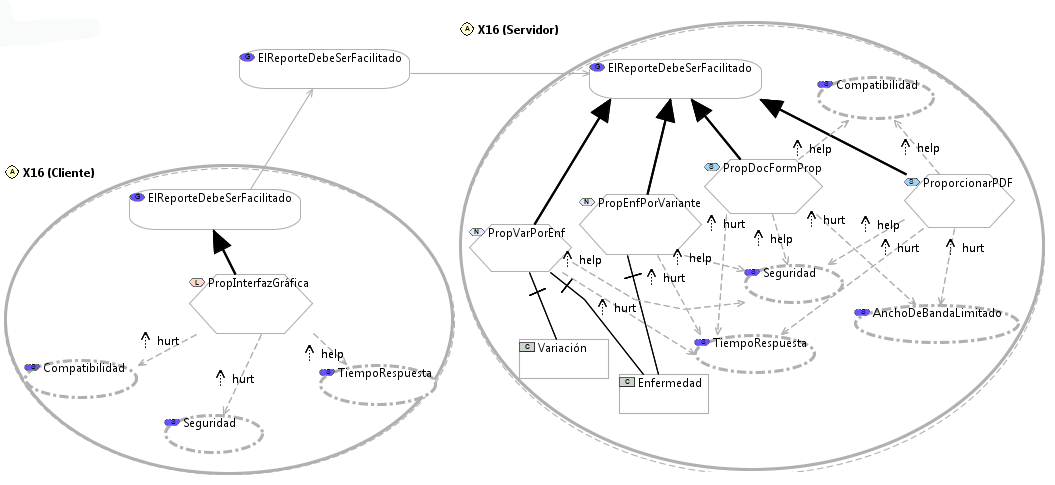
\includegraphics[width=1.5\textwidth]{img/X16.png}
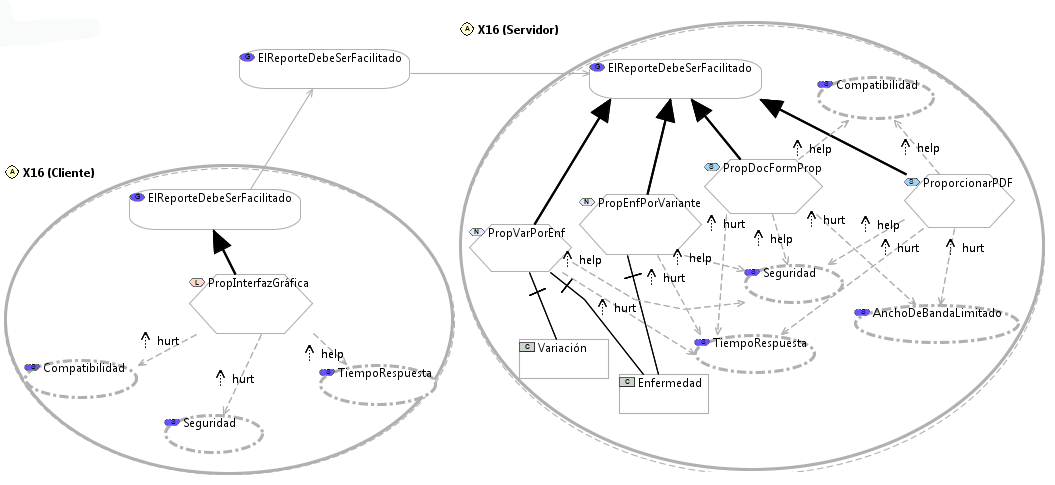
\includegraphics[width=18.5cm,height=12.5cm]{img/X16.png}
\end{center}
\caption{Configuraci�n X16: distribuci�n de los requisitos entre el cliente y el servidor.} \label{fig:X16}
\end{figure}
\end{landscape}
	
	
\item \textbf{\textit{Secci�n \ref{imp:transformaciones}:}} ``Transformaciones Modelo a Modelo''. La secci�n permite satisfacer el objetivo 3 de la tesis doctoral, gracias a que por medio de las transformaciones modelo a modelo es posible la generaci�n de las estructuras de los modelos conceptuales de la aplicaci�n Web, que posteriormente, deber�n ser completados por el dise�ador. Por lo tanto, la secci�n \ref{imp:transformaciones} ofrece un alto grado de automatizaci�n en el desarrollo de aplicaciones Web por medio de un conjunto de transformaciones y con esto brinda soporte a la generaci�n de c�digo. Para m�s informaci�n consultar los art�culos listados en la secci�n \ref{otraspub} y el Cap�tulo \ref{c4} de la tesis doctoral.

\item \textbf{\textit{Secci�n \ref{imp:trazabilidad}:}} ``Trazabilidad de Requisitos''. La secci�n proporciona el soporte necesario para satisfacer el objetivo especifico 4 de la secci�n \ref{c1s1} de la tesis. Por medio de las transformaciones modelo a modelo es posible ofrecer al dise�ador soporte para trazabilidad de requisitos. Para m�s informaci�n consultar los art�culos listados en la secci�n \ref{otraspub} y el Cap�tulo \ref{c5} de la tesis doctoral.

\item \textbf{\textit{Secci�n \ref{imp:pareto}:}} ``Optimizaci�n de Pareto''. La implementaci�n que complementa la tesis doctoral cumple con el objetivo 5 de la secci�n \ref{c1s1}. B�sicamente, el apartado \ref{imp:pareto} asiste al dise�ador de la aplicaci�n Web al momento de la selecci�n de los requisitos funcionales a implementar a trav�s de alternativas de dise�o que consideren el balance y maximizaci�n de los requisitos no-funcionales. Para m�s informaci�n consultar el Cap�tulo \ref{c6} y el Ap�ndice \ref{a3} de la tesis.

\end{itemize}
   
Por otra parte, la propuesta presentada en la tesis doctoral ha seguido un proceso de desarrollo basado en MDA. Por lo tanto, para llevar a cabo la implementaci� ha sido necesaria combinaci�n de un conjunto de tecnolog�as MDD entre las que destacan (i) la plataforma de desarrollo \emph{Eclipse}~\cite{ECLIPSE}, (ii) la tecnolog�a EMF (\emph{Eclipse Modeling Framework}) \cite{EMF} y GMF (\emph{Graphical Modeling Framework}) \cite{GMF} y (iii) el lenguaje para transformaciones entre modelos ATL (\emph{Atlas Transformation Language}) \cite{ATL}. Cada una de las tecnolog�as utilizadas son descritas a continuaci�n.



%La propuesta definida en esta tesis doctoral se ha implementado en la plataforma de desarrollo \emph{Eclipse}~\cite{ECLIPSE} utilizando tecnolog�a EMF (\emph{Eclipse Modeling Framework}) (CITA) y GMF (\emph{Graphical Modeling Framework}) (CITA). \emph{Eclipse} puede extenderse por medio de \emph{plugins} con el fin de a�adir m�s caracter�sticas y nuevas funcionalidades. Se ha desarrollado un \emph{plugin} que da soporte a cada parte de la propuesta. Este nuevo plugin contiene los siguientes m�dulos:

\begin{itemize}
   \item \textbf{\emph{Eclipse}}. Es un entorno de desarrollo integrado (\emph{Integrated Development Enviroment}, IDE) de c�digo abierto multiplataforma, fue desarrollado originalmente por IBM\footnote{\url{http://www-01.ibm.com/software/rational/eclipse/}}. \emph{Eclipse} es ahora desarrollado por la Fundaci�n \emph{Eclipse}, una organizaci�n independiente sin �nimo de lucro que fomenta una comunidad de c�digo abierto. La caracter�stica principal del IDE es que es  una plataforma de programaci�n utilizada para crear entornos integrados de desarrollo que puede ser extendida por medio de \emph{plugins} con el fin de a�adir m�s caracter�sticas y nuevas funcionalidades. 
   
	\item \textbf{\emph{Eclipse Modeling Framework (EMF)}}. Es un marco de trabajo para modelado que ofrece facilidad de generaci�n de c�digo para construir herramientas y otras aplicaciones basadas en un modelo de datos estructurado. Desde una especificaci�n del modelo descrita en XMI (XML de Intercambio de Metadatos), \emph{EMF} suministra herramientas y soporte en tiempo de ejecuci�n para producir un conjunto de clases Java para el modelo, un conjunto de clases del tipo \emph{Adapter} que permiten visualizaci�n y edici�n bas�ndose en comandos del modelo, y un editor b�sico. Los modelos pueden ser especificados usando notaci�n Java, documentos XML, o herramientas de modelado como \emph{Rational Rose}\footnote{http://www-01.ibm.com/software/awdtools/developer/rose/}, y despu�s ser importados a \emph{EMF}. Lo m�s importante de todo, \emph{EMF} suministra las bases para la interoperabilidad con otras herramientas y aplicaciones basadas en \emph{EMF}. Dentro de \emph{EMF} encontramos un metamodelo para describir modelos llamado Ecore, este metamodelo incluye soporte en tiempo de ejecuci�n para los modelos adem�s de notificaci�n de cambios.
	
	\item \textbf{\emph{Graphical Modeling Framework (GMF)}}. Es un marco de trabajo que permite el desarrollo de editores gr�ficos. GMF combina EMF y GEF (\emph{Graphical Editing Framework}) para el desarrollo de editores gr�ficos \textit{ad-hoc}. De tal forma que, los elementos creados con el editor gr�fico, son una representaci�n visual de cada concepto especificado en el metamodelo.
	
	\item \textbf{\emph{Atlas Transformation Language (ATL)}}. Es un lenguaje de transformaci�n de modelos basado en los est�ndares del
OMG \cite{OMG} y OCL 2.0 \cite{OCL}. ATL es un lenguaje declarativo e imperativo (h�brido) que permite la transformaci�n entre modelos (M2M). Las construcciones declarativas son la opci�n preferida para escribir las transformaciones debido a que permiten expresar correspondencias, entre los elementos del modelo fuente y del modelo destino a partir de una serie de composiciones de reglas. Las construcciones imperativas proporcionan constructores para facilitar la especificaci�n de correspondencias que de forma declarativa ser�an m�s complejas de implementar.

\item \textbf{\emph{Xpand}}. Es un lenguaje especializado en la generaci�n de c�digo a partir de modelos EMF \cite{Xpand}. Xpand ofrece la posibilidad de escribir completas librerias de funciones para la lectura de modelos EMF y permite la utilizaci�n de las librerias de funciones desde c�digo Java \cite{Java} o expresiones Xtend.
     \item \textbf{\emph{Java}}. Es un lenguaje de programaci�n orientado a objetos, dise�ado principalmente para tener el m�nimo de dependencia del sistema operativo para su utilizaci�n. Actualmente, Java es uno de los lenguajes de programaci�n m�as populares \cite{Java}.
\end{itemize}

Finalmente, en el apartado \ref{imp:casoestudio} de esta secci�n se presenta un caso de estudio para ejemplificar la aplicabilidad de nuestra propuesta. En el caso de estudio, se detalla la especificaci�n de requisitos Web por medio del marco de modelado \emph{i*}, el soporte para trazabilidad de requisitos y la selecci�n de las distintas alternativas de implementaci�n de los requisitos funcionales mediante la optimizaci�n de las \emph{Softgoals}.

\subsection{Editor Gr�fico para la Especificaci�n de Requisitos Web (\emph{WebREd})}\label{subseccioneditor}

En este apartado son implementados los conceptos (sintaxis abstracta) del marco de modelado \emph{i*} y la clasificaci�n de requisitos presentada en el Cap�tulo \ref{especificacion} de la tesis para proveer al dise�ador con un editor gr�fico para la especificaci�n de requisitos Web. Como se mencion� anteriormente, la propuesta presentada en la tesis doctoral se encuentra alineada con MDA, por lo tanto, el editor WebREd corresponde al modelo independiente de computaci�n (CIM). Concretamente, el metamodelo de requisitos implementado en la tesis doctoral ha sido extendido para incorporar los tipos de requisitos de \emph{i*} y la clasificaci�n presentada en la secci�n \ref{especificacion}. La Figura \ref{fig:SeccionRequisitosWebMetamodelo} muestra una captura de pantalla donde puede apreciarse la implementaci�n del metamodelo en \emph{Eclipse}. La sint�xis concreta del metamodelo para requisitos Web se ha implementado para desarrollar un editor gr�fico (Figura \ref{fig:herramienta}) por medio de la tecnolog�a GMF. 

\begin{figure}
\begin{center}
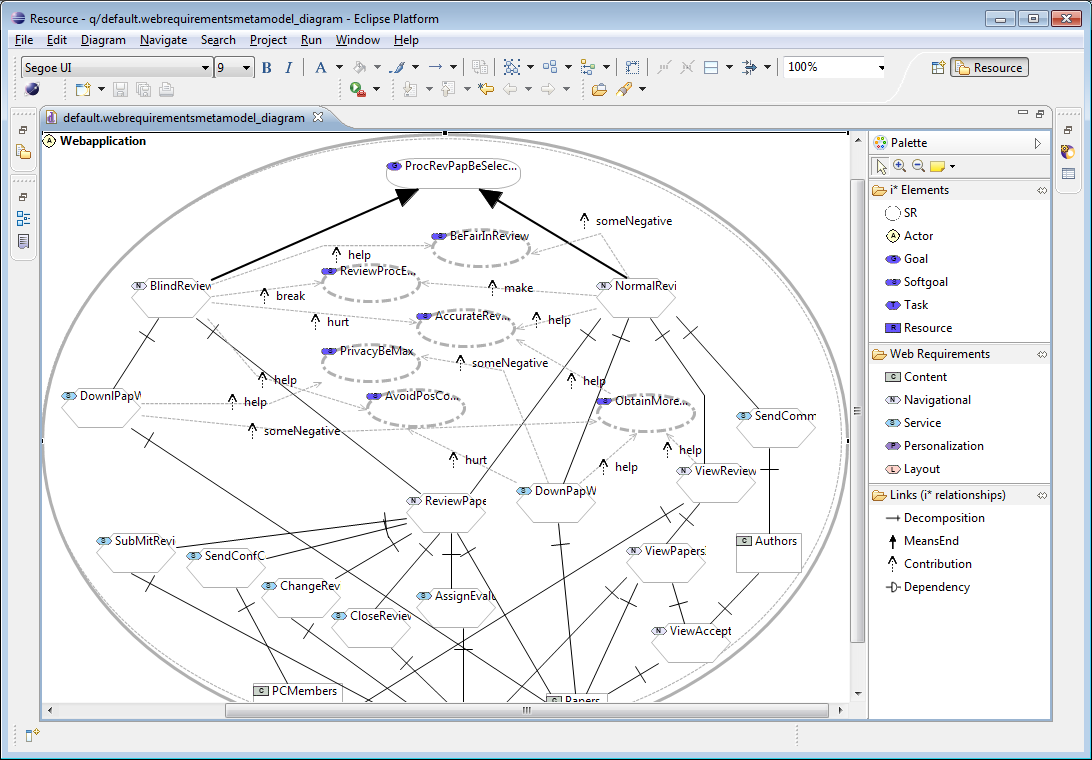
\includegraphics[width=\textwidth]{img/Herramienta.png}
\end{center}
\caption{Editor WebREd para la especificaci�n de requisitos Web con \emph{i*}.}
\label{fig:herramienta}
\end{figure}

El editor (Figura \ref{fig:herramienta}) WebREd (\emph{Web Requirements Editor}) brinda al dise�ador de la aplicaci�n Web una interfaz gr�fica para especificar en un diagrama los requisitos funcionales y las \emph{Softgoals} de la aplicaci�n Web. WebREd permite la creaci�n, modificaci�n y actualizaci�n de la especificaci�n de requisitos Web (diagramas). Adem�s, cada una de las propiedades de los elementos del marco de modelado \emph{i*} pueden ser modificadas seleccionando cada elemento en la vista de propiedades (Figura \ref{fig:PropViewWebREd}). 

\begin{figure}
\begin{center}
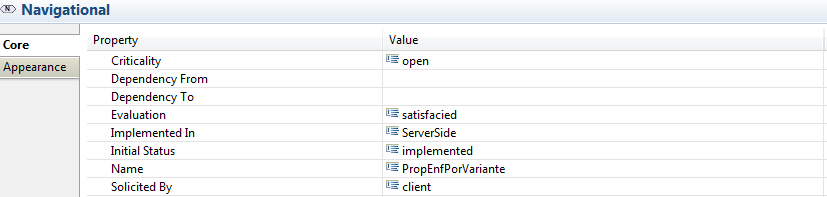
\includegraphics[width=\textwidth]{img/PropViewWebREd.png}
\end{center}
\caption{Vista de propiedades del editor WebREd.}
\label{fig:PropViewWebREd}
\end{figure}

Es importante destacar que adem�s de poder especificar modelos de requisitos Web (\emph{Content}, \emph{Navigational}, \emph{Personalization}, \emph{Service} y \emph{Layout}), WebREd permite la creaci�n de diagramas (modelos orientados a objetivos) com�nes de \emph{i*} gracias a que coloca a disposici�n del dise�ador los elementos cl�sicos (\emph{Goal}, \emph{Task}, \emph{Resource} y \emph{Softgoal}) del marco de modelado \emph{i*} como puede verse en la Figura \ref{fig:paleta}, en donde se muestran los elementos que permiten la creaci�n de cada elemento \emph{i*} realizando un \emph{drag and drop} de cada elemento sobre el diagrama. 


\begin{figure}
\begin{center}
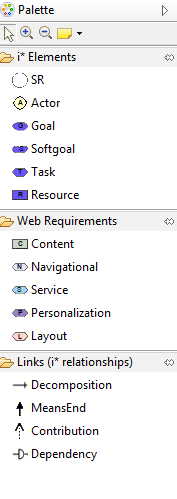
\includegraphics[width=0.3\textwidth]{img/paleta.png}
\end{center}
\caption{Elementos para el dise�o del modelo de requisitos Web con \emph{i*}.}
\label{fig:paleta}
\end{figure}


\subsection{Transformaciones Modelo a Modelo}\label{imp:transformaciones}

Con el fin de aprovechar cada una de las ventajas que ofrece la ingenier�a dirigida por modelos y con esto automatizar el paso del CIM al PIM, se han desarrollado una serie de reglas de transformaci�n definidas formalmente en el lenguaje QVT (secci�n \ref{reglas}). Con esta idea, las transformaciones deben de ser vistas desde una perspectiva de modelado como modelos de transformaciones \cite{bezivin2006model}. En la investigaci�n asociada a la tesis doctoral, QVT se ha utilizado como metamodelo para formalizar las transformaciones modelo a modelo abstray�ndolas como modelos, con el fin de mejorar la comprensi�n del proceso de transformaci�n. Sin embargo, una vez que las transformaciones han sido modeladas, necesitan implementarse. Como se ha mencionado anteriormente, se ha utilizado el lenguaje ATL para implementar cada una de las reglas definidas en la secci�n \ref{reglas} y de esta forma ejecutarlas con el fin de realizar el proceso de normalizaci�n de forma autom�tica. Cabe destacar que utilizar ATL para implementar transformaciones QVT es factible debido a la alineaci�n que existe entre la arquitectura de ambos de lenguajes \cite{jouault2006architectural}.

La Figura \ref{fig:Content2DomainClass} muestra el c�digo ATL referente a la implementaci�n de la regla \emph{Content2DomainClass} (descrita en detalle en la secci�n \ref{reglas}). La regla tiene como objetivo crear las clases del modelo de dominio de A-OOH.

%El metamodelo de navegaci�n en A-OOH se implementa en este m�dulo. El metamodelo definido formalmente en la Figura \ref{fig:navmetamodel} define la sintaxis abstracta para la representaci�n conceptual en un PIM del modelo de navegaci�n de A-OOH.

\begin{figure}
\begin{center}
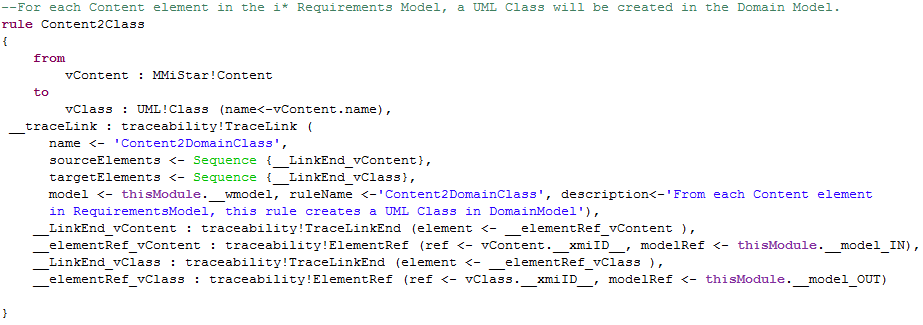
\includegraphics[width=\textwidth]{img/Content2DomainClasATL.png}
\end{center}
\caption{Implementaci�n de la transformaci�n \emph{Content2DomainClass} en el lenguaje ATL.}
\label{fig:Content2DomainClass}
\end{figure}

\subsection{Trazabilidad de Requisitos}\label{imp:trazabilidad}

El soporte para la trazabilidad de los requisitos a trav�s de los modelos conceptuales de la aplicaci�n Web se efect�a por medio de una extensi�n \cite{barbero2007traceability} del metamodelo de \emph{weaving}, explicado previamente en la secci�n \ref{c1:trazabilidad} de la tesis doctoral. La extensi�n para trazabilidad del metamodelo de \emph{weaving} permite generar por medio de transformaciones un modelo de trazabilidad. El modelo de trazabilidad puede ser visualizado y modificado mediante la herramienta AMW (\emph{Atlas Model Weaver}) \cite{del2006weaving}. De esta forma, es posible visualizar las correspondencias entre cada uno de los requisitos funcionales expresados en el modelo de requisitos \emph{i*} con cada uno de los elementos de los modelos conceptuales de la aplicaci�n Web  \cite{aguilarDSDM}.

\subsection{Optimizaci�n de Pareto}\label{imp:pareto}

El algoritmo Optimizaci�n de Pareto ha sido implementado por medio del lenguaje de programaci�n Java. Adicionalmente, ha sido necesario el uso de las clases base (\emph{core}) de EMF y el lenguaje Xpand con el fin de ser capaz de leer el modelo de requisitos \emph{i*}. El algoritmo se ha implementado como un \emph{plugin} de Eclipse para su f�cil incorporaci�n con el editor WebREd. 

La Optimizaci�n de Pareto es calculada en 3 pasos, el primero de ellos consiste en establecer la lista de prioridades para las \emph{Softgoals}, es decir, el dise�ador ordenar� las \emph{Softgoals} indicando cual es la de mayor importancia de acorde a lo establecido por los \emph{stakeholders}. En el segundo paso, son extra�dos los requisitos funcionales as� como las contribuciones que estos realizan a las \emph{Softgoals} y en el tercer paso se calcula la Optimizaci�n de Pareto. La Figura \ref{fig:imp:paretomain} muestra la ventana principal de la implementaci�n del algoritmo.  La ventana esta dividida en 3 pesta�as (\emph{Configuration}, \emph{Requirements Contributions}, \emph{The Pareto Front}), cada una de ellas corresponde a los 3 pasos necesarios para la ejecuci�n del algoritmo. 

\begin{figure}
\begin{center}
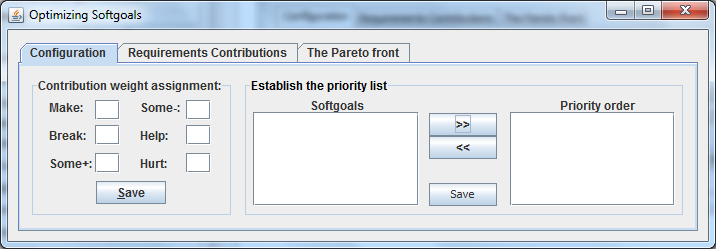
\includegraphics[width=\textwidth]{img/ParetoMainWindowImple.png}
\end{center}
\caption{Ventana principal del \emph{plugin} Optimizaci�n de Pareto.}
\label{fig:imp:paretomain}
\end{figure}


\subsection{Caso de estudio}\label{imp:casoestudio}

En este apartado se presenta un caso de estudio para demostrar la aplicabilidad de nuestra propuesta. El caso de estudio es el utilizado en el Cap�tulo \ref{c6} acerca de una aplicaci�n Web para la gesti�n de conferencias (\emph{Conference Management System}). Recordemos que el prop�sito de la aplicaci�n Web es brindar soporte al proceso de env�o, evaluaci�n y selecci�n de los art�culos para una conferencia. 

%Para efectos demostrativos, en este caso de estudio nos enfocaremos en la obtenci�n del modelo de dominio, navegaci�n y trazabilidad a partir de la especificaci�n de requisitos.

El primer paso consiste en la especificaci�n de los requisitos para la aplicaci�n Web ``\emph{ContentManagementSystem}''. La Figura \ref{fig:imp:reqcasoestudio}, muestra la especificaci�n de requisitos de la aplicaci�n Web (modelo de requisitos). El objetivo de la aplicaci�n Web consiste en ``\emph{Process of review of papers be selected}'', para satisfacer el objetivo, es necesario la implementaci�n de alguno de los requisitos navegacionales ``\emph{Blind review process}'' y ``\emph{Normal review process}''. En el ejemplo el objetivo es logrado a trav�s del requisito navegacional ``\emph{Blind review process}''. 

\begin{figure}
\begin{center}
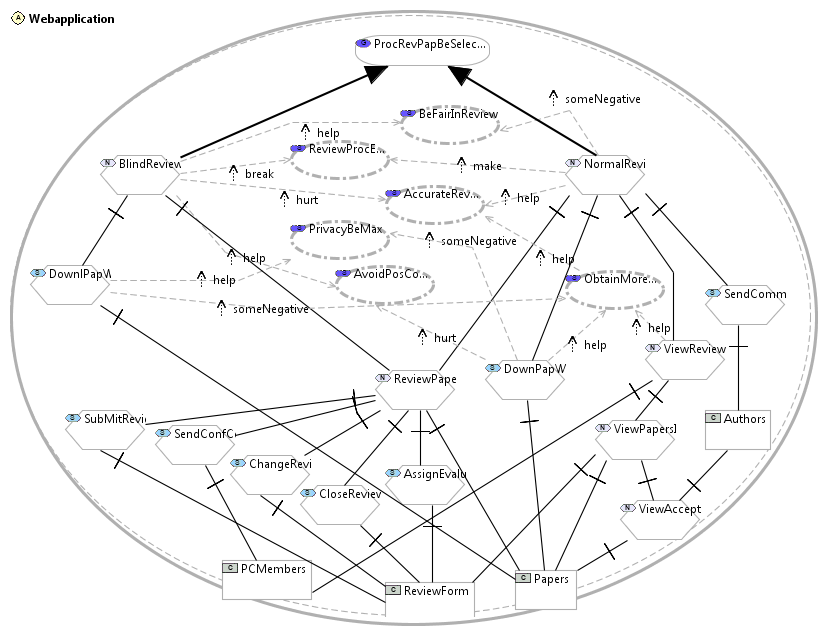
\includegraphics[width=\textwidth]{img/EjemploImplementacionTesisRequisitos.png}
\end{center}
\caption{Especificaci�n de requisitos Web con \emph{i*} para el caso de estudio.}
\label{fig:imp:reqcasoestudio}
\end{figure}

El siguiente paso consiste en ejecutar las reglas de transformaci�n para derivar autom�ticamente la estructura del modelo de dominio de A-OOH. En la Figura \ref{fig:imp:Service2ClassOperationATL} se muestra la regla de transformaci�n \emph{Service2ClassOperation} (definida en la secci�n \ref{reglas}) implementada en ATL. 

\begin{figure}
\begin{center}
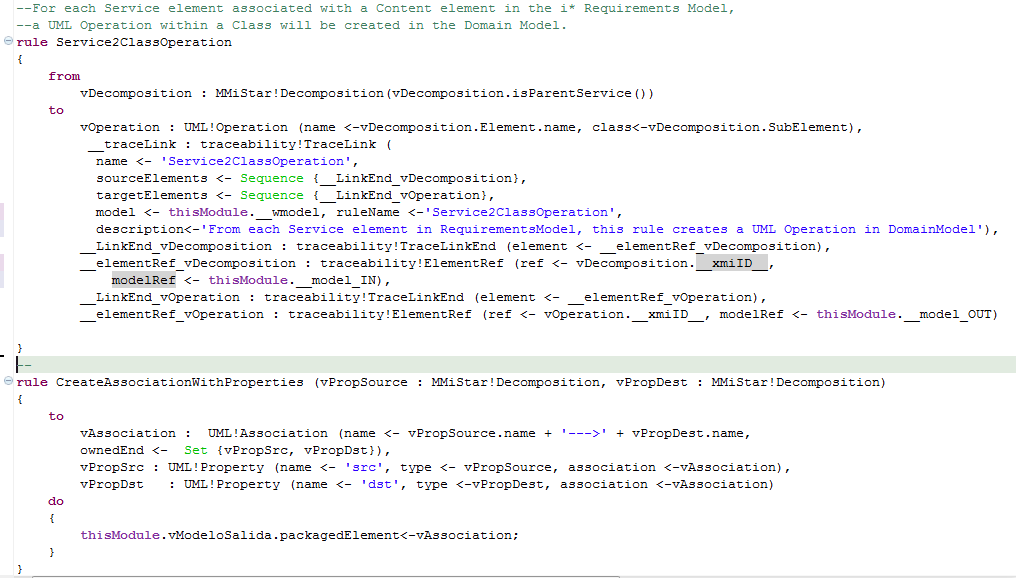
\includegraphics[width=\textwidth]{img/Service2ClassOperationATL.png}
\end{center}
\caption{Reglas ATL para obtener las operaciones de las clases del modelo de dominio A-OOH.}
\label{fig:imp:Service2ClassOperationATL}
\end{figure}

En este caso de estudio, el modelo de dominio de A-OOH se muestra en la Figura \ref{fig:imp:DomainModelCaseStudy}. Como se puede observar, el modelo esta constituido por un \emph{UML-Package}, dentro del cual se encuentran los elementos comunes de un diagrama de clases UML tales como las clases, las operaciones dentro de las clases y las asociaciones.

\begin{figure}
\begin{center}
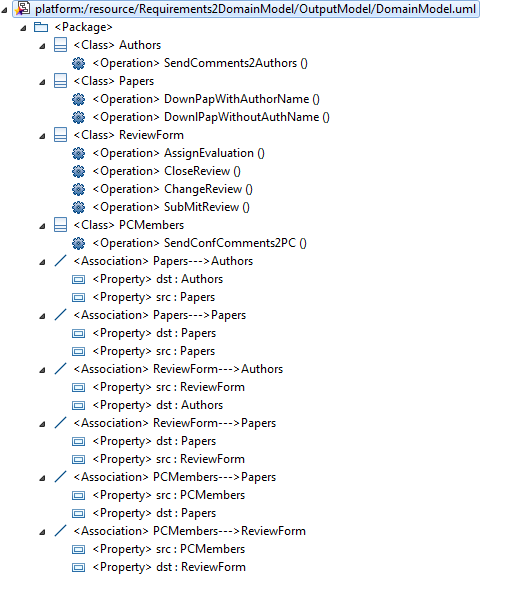
\includegraphics[width=0.9\textwidth]{img/DomainModelCaseStudy.png}
\end{center}
\caption{Modelo de dominio A-OOH.}
\label{fig:imp:DomainModelCaseStudy}
\end{figure}

El pr�ximo paso es la obtenci�n de la estructura del modelo de navegaci�n de A-OOH. Para esto se han implementado en ATL (Figura \ref{fig:imp:CreateNavigationalModelATL}) las reglas de transformaci�n presentadas en la secci�n \ref{reglas}. El proceso de derivaci�n de un modelo de navegaci�n permite obtener un modelo conceptual donde se especifiquen las rutas que el usuario de la aplicaci�n Web podr� utilizar para desplazarse por el contenido. En la Figura \ref{fig:imp:NavigationalMetamodelCaseStudy} se muestra el modelo de navegaci�n obtenido autom�ticamente a partir del modelo de requisitos. Como se describio en la secci�n \ref{modelos}, el modelo de navegaci�n esta constituido por clases navegacionales, enlaces navegacionales y nodos navegacionales. 

\begin{figure}
\begin{center}
\includegraphics[width=\textwidth]{img/CreateNavigationalModelATL.png}
\end{center}
\caption{Extracto de la regla ATL para obtener el modelo de navegaci�n.}
\label{fig:imp:CreateNavigationalModelATL}
\end{figure}


%\begin{landscape}
\begin{figure}
\begin{center}
\includegraphics[width=\textwidth]{img/NavigationalMetamodelCaseStudy.png}
\end{center}
\caption{Modelo de navegaci�n del caso de estudio.}
\label{fig:imp:NavigationalMetamodelCaseStudy}
\end{figure}
%\end{landscape}

Al mismo tiempo que ocurre la generaci�n de los modelos de dominio y navegaci�n de A-OOH se obtiene el modelo de trazabilidad (Secci�n \ref{c1:trazabilidad}). Esto es debido a que las reglas para crear los enlaces para trazabilidad est�n introducidas en las reglas ATL que derivan los modelos conceptuales. La Figura \ref{fig:imp:TraceModelReqDomain} muestra la parte de la transformaci�n ATL donde se genera el modelo de trazabilidad dentro de la regla de transformaci�n que derivan el modelo de dominio.

\begin{figure}
\begin{center}
\includegraphics[width=\textwidth]{img/TraceModelReqDomain.png}
\end{center}
\caption{Extracto de la regla ATL para obtener el modelo de dominio en donde se crea el modelo de trazabilidad.}
\label{fig:imp:TraceModelReqDomain}
\end{figure}

El pr�ximo paso consiste en visualizar el modelo de trazabilidad obtenido por medio de la herramienta AMW \emph{Atlas Model Weaver}  \cite{AtlasModelWeaver}. AMW es una herramienta que permite visualizar los enlaces contenidos en los modelos de \emph{weaving}. En la Figura \ref{fig:imp:TrazabilidadAtlasModelWeaver} se muestra el soporte para trazabilidad de A-OOH, en el lado izquiero de la imagen se visualiza el modelo de requisitos, al centro el modelo de trazabilidad y en el lado derecho se puede observar el modelo de dominio. Cuando el dise�ador selecciona alg�n elemento de cualquier modelo (requisitos, trazabilidad o dominio) la herramienta resalta los respectivos elementos con los que corresponde el elemento seleccionado. Por �ltimo, en la parte inferior de la figura se pueden ver las propiedades de los elementos del modelo de trazabilidad.


Como se explic� en la secci�n \ref{modelos} de la tesis doctoral, una vez que han sido obtenidos las estructuras de los modelos de dominio y navegaci�n el dise�ador solo tendr� que refinarlos, por ejemplo, en el modelo de dominio el usuario tendr� que a�adir de forma manual la cardinalidad de las asociaciones entre las clases. M�s informaci�n se detalla en el Cap�tulo \ref{c4} de la tesis.

Una vez que se tiene un prototipo inicial de los modelos conceptuales de la aplicaci�n, vamos a suponer que el dise�ador necesita optimizar la seguridad de la aplicaci�n Web debido a una solicitud expresa de los \emph{stakeholders}. Para esto, necesita la ejecuci�n del \emph{plugin} Optimizaci�n de Pareto y con ello obtener como resultado un conjunto de configuraciones que le permitan saber que requisitos funcionales implementar de acuerdo a las \emph{Softgoals} que se necesiten optimizar. 

\begin{landscape}
\begin{figure}
\begin{center}
%\includegraphics[width=1.5\textwidth]{img/TrazabilidadAtlasModelWeaver.png}
\includegraphics[width=18.5cm,height=13.5cm]{img/TrazabilidadAtlasModelWeaver.png}
\end{center}
\caption{Visualizaci�n del modelo de trazabilidad en la herramienta AMW.}
\label{fig:imp:TrazabilidadAtlasModelWeaver}
\end{figure}
\end{landscape}

El \emph{plugin} para la Optimizaci�n de Pareto utiliza como modelo de entrada el modelo de requisitos \emph{i*}, as�, por medio de las clases EMF y el lenguaje Xpand el modelo de requisitos es le�do para extraer todos los requisitos, \emph{Softgoals} y los enlaces de contribuci�n (\emph{contribution links}) contenidos en el. La Figura \ref{fig:imp:paretomainwithdata} muestra la ventana principal del \emph{plugin}, la cual contiene un \emph{tab pane} dividido en 3 pesta�as (\emph{tabs}). La primera pesta�a se llama \emph{Configuration}, en el costado izquierdo el dise�ador puede cambiar los valores establecidos por \emph{default} que representan la fuerza de las contribuciones realizadas por parte de los requisitos funcionales a las \emph{Softgoals}, los valores son utilizados en el c�lculo de la matriz de pesos (Secci�n \ref{c1:optimizacion}). En el costado derecho de la misma figura se muestra la secci�n en donde el dise�ador establece la lista de prioridades de \emph{Softgoals}. En este caso de estudio, el dise�ador necesita maximizar la \emph{Softgoal} \emph{Privacy Be Maximized} que es la relacionada con la seguridad de la aplicaci�n Web.


\begin{figure}
\begin{center}
\includegraphics[width=\textwidth]{img/ParetoMainWindow.png}
\end{center}
\caption{Ventana principal del \emph{plugin} Optimizaci�n de Pareto (pesta�a de configuraci�n).}
\label{fig:imp:paretomainwithdata}
\end{figure}

En la Figura \ref{fig:imp:paretosegundapestana} se muestra la pesta�a \emph{Requirements Contributions} en donde se puede ver en un listado el resultado del \emph{plugin} al extraer del modelo de requisitos \emph{�*} aquellos requisitos funcionales que realicen alg�n tipo de contribuci�n a las \emph{Softgoals}. En la primera columna se encuentran listados los requisitos funcionales extra�dos, cabe destacar que los requisitos funcionales listados son solo aquellos que realizan contribuciones a las \emph{Softgoals} independientemente de su estado, es decir, si se encuentran implementados o no en los modelos conceptuales de la aplicaci�n Web. Las 6 columnas restantes corresponden con cada una de las \emph{Softgoals} extra�das del modelo de requisitos. Finalmente, en la parte inferior de la pesta�a \emph{Requirements Contributions} se encuentra el bot�n para calcular el resultado del algoritmo Optimizaci�n de Pareto, es decir la Frontera de Pareto.

\begin{figure}
\begin{center}
\includegraphics[width=\textwidth]{img/ParetoSecondWindow.png}
\end{center}
\caption{\emph{Plugin} Optimizaci�n de Pareto. Las contribuciones de los requisitos a las \emph{Softgoals}.}
\label{fig:imp:paretosegundapestana}
\end{figure}

El resultado de la  ejecuci�n del algoritmo se puede ver en la Figura \ref{fig:imp:paretotercerapestana}. La pesta�a \emph{The Pareto Front} muestra una tabla similar a la descrita en la secci�n \ref{c1:optimizacion} en donde son mostrados los resultados de la ejecuci�n del algoritmo. Las configuraciones posibles se enlistan desde la primera columna llamada \emph{Configurations} hasta la columna 6, la variable ``I'' representa el estado implementado para un requisito funcional determinado y la variable ``N'' significa que ese requisito funcional no debe de ser implementado en los modelos conceptuales de la aplicaci�n Web. Las configuraciones que est�n en la Frontera de Pareto se resaltan en color gris para que sean f�ciles de identificar por parte del dise�ador.


\begin{figure}
\begin{center}
\includegraphics[width=\textwidth]{img/ParetoThirdWindow.png}
\end{center}
\caption{\emph{Plugin} Optimizaci�n de Pareto. La Frontera de Pareto.}
\label{fig:imp:paretotercerapestana}
\end{figure}

El dise�ador asistido por la tabla de la Frontera de Pareto (Figura \ref{fig:imp:paretotercerapestana}) podr� ser capaz de seleccionar la configuraci�n final de acuerdo con la lista de prioridades de las \emph{Softgoals}. En este caso de estudio, para maximizar la seguridad de la aplicaci�n Web, el dise�ador podr� elegir entre las configuraciones ``X3'' y ``X7''. 

Finalmente,, la opci�n a implementar es la configuraci�n ``X3'' debido a que la configuraci�n ``X7'' maximiza la \emph{Softgoal} relacionada con la seguridad (+1) pero afecta demasiado (-4) a la \emph{Softgoal} \emph{Review Process Easier} la cual esta vinculada con la usabilidad de la aplicaci�n. La configuraci�n ``X8'' no es considerada por que no est� en la Frontera de Pareto.

Una explicaci�n m�s a fondo sobre el funcionamiento del algoritmo Optimizaci�n de Pareto y su adaptaci�n a la ingenier�a Web dirigida por modelos se encuentra en el Cap�tulo \ref{c6} y en el Ap�ndice \ref{a3} de la tesis doctoral.


\clearpage


\section{Conclusiones}

La Web cambia constantemente debido a la evoluci�n constante en las tecnolog�as de implementaci�n. Por tanto, las metodolog�as ingenier�les necesitan adaptarse a los cambios con el fin de ofrecer al dise�ador una aproximaci�n sistem�tica e integral para el desarrollo de aplicaciones Web. Adem�s, debido a la naturaleza cambiante de la Web y a su audiencia heterog�nea, mantener una etapa de an�lisis y especificaci�n de requisitos resulta cada vez m�s complicado. 

Para tratar con estas cuestiones, en esta tesis doctoral, se ha
presentado una propuesta dirigida por modelos que permite (i) la
especificaci�n de un modelo de requisitos a nivel conceptual de manera
integral, sistem�tica y bien estructurada y (ii) la derivaci�n
autom�tica de los modelos conceptuales de dominio y navegaci�n. Por lo tanto, la propuesta permite a los dise�adores disminuir el nivel de complejidad en el desarrollo de aplicaciones Web, ahorrando tiempo y esfuerzo con lo que el costo del proyecto disminuye. Posteriormente, se ha a�adido a la propuesta dirigida por modelos un soporte al dise�ador por medio de una gesti�n integral de requisitos con el fin de asegurar la la trazabilidad de los requisitos de CIM a PIM, an�lisis de impacto y la implementaci�n de requisitos funcionales en base a distintas alternativas de dise�o considerando la maximizaci�n de los requisitos no-funcionales. Tambi�n, se ha realizado una implementaci�n en \emph{Eclipse} para apoyar cada parte de esta propuesta.

Finalmente, cabe destacar que la tesis doctoral representa la
primera propuesta dirigida por modelos en ingenier�a Web que aplica un marco de trabajo orientado a objetivos para la etapa de an�lisis y especificaci�n de requisitos en un contexto MDA, a la vez permite la generaci�n de los modelos conceptuales de la aplicaci�n Web en un proceso con un alto grado de automatizaci�n.

%\textbf{Not only an approach that deals with the MD modeling of DWs
%has been defined but also a general framework to align the
%development of every part of a DW with MDA (see chapter~\ref{c3}),
%thus paving the way for future research objectives as the modeling
%of ETL process or data analysis tools...}

\clearpage



\bibliographystyle{abbrv}
\bibliography{tesis}


%

%%%%%%%%%%%%%%%%%%%%%% chapter2.tex %%%%%%%%%%%%%%%%%%%%%%%%%%%%%%%%%
%
% Summary chapter.
%
%
%%%%%%%%%%%%%%%%%%%%%%%% Universidad de Alicante %%%%%%%%%%%%%%%%%%%%%%%%%%
\chapter{Summary in English}
\label{c2} % Always give a unique label
% use \chaptermark{}
% to alter or adjust the chapter heading in the running head

This PhD Thesis is composed of a set of published and submitted
papers. Therefore, this chapter is devoted to a description of
initial hypotheses, research objectives, and the collection of works
that are part of this Thesis, thus justifying its coherence. It
should be underlined that this chapter summarizes the scientific
content of this PhD Thesis, including research results and final
conclusions. Finally, the previous chapter has been written in
Spanish, and then translated into English as follows.

\section{PhD Thesis as a Collection of Papers}

In order to write this PhD Thesis as a collection of papers in the
University of Alicante, a set of requirements must be followed.
These requirements were defined by \emph{``Pleno de la Comisi�n de
Doctorado de la Universidad de Alicante''} on the 2nd of March,
2005; those related to the content of the PhD Thesis are presented
as follows:

\begin{enumerate}

\item \emph{``The PhD Thesis must include a summary written in one of the two official
languages of this region. It should contain objectives, hypotheses
and works to justify the coherence of the research.''}

\item \emph{``This summary must include an abstract to present the results, a discussion of them and the final
conclusions. This summary must give an idea of the overall content
of the PhD Thesis.''}

\item \emph{``The works presented in this PhD Thesis must be
published or accepted for publication after the beginning of the
PhD. Papers under review  can be included in the appendices of the
PhD Thesis.''}

\end{enumerate}

In order to fulfil the aforementioned requirements, this PhD Thesis
is structured in three parts. Part~\ref{p1} consists of a summary in
Spanish (Chapter~\ref{c1}) and its corresponding summary in English
(Chapter~\ref{c2}). Part~\ref{p2} presents a collection of published
papers. Part~\ref{p3} is an appendix which contains the papers that
are currently under the review process. Finally, it is worth
mentioning that this PhD Thesis has been developed thanks to the
funding of the Spanish Ministry of Education and Science under the
FPU grant program. In order to apply for this kind of grants, a
project for a PhD Thesis must be presented. Each research
publication is consequently a fundamental part of the global work,
forming a coherent collection.


\subsection{Publications Included in this PhD Thesis}
\label{c2:chapter} Four of the published research papers have been
selected to be part of this PhD Thesis due to (i) their scientific
contribution and (ii) their relevance. They are described in this
section.

\subsubsection{Chapter~\ref{c3}}

\emph{J.-N. Maz{\'o}n, J. Trujillo. An MDA approach for the
development of data warehouses. Decision Support Systems,
45(1):41--58, 2008. [IF2007: 1.119].}

This work describes a standard and integrated model-driven framework
for designing each component of a data warehouse. Once this
framework has been defined, the focus is on the multidimensional
modeling of the data warehouse repository. This work specifically
defines a conceptual multidimensional model and how it is translated
to a relational-based logical representation by using a model-driven
approach. The advantages of using the model-driven development to
design data warehouses are also enumerated.



\subsubsection{Chapter~\ref{c4}}

\emph{J.-N. Maz{\'o}n, J. Pardillo, J. Trujillo. Applying
Transformations to Model Driven Data Warehouses. 8th International
Conference on Data Warehousing and Knowledge Discovery (DaWaK 2006),
Krakow (Poland), September 4-8, 2006. Lecture Notes in Computer
Science Vol. 4081, pp. 13--22. [Acceptance rate: 36.3\%].}

Since the previous work had defined how to obtain a relational-based
implementation of the multidimensional conceptual model, this paper
focused on obtaining a logical representation directly based on
multidimensional technology, thus showing the full potential of
applying formal transformations within a model-driven approach,
thereby allowing designers to automatically implement it in any
commercial platform.


\subsubsection{Chapter~\ref{c5}}

\emph{J.-N. Maz{\'o}n, J. Trujillo, J. Lechtenb{\"o}rger.
Reconciling requirement-driven data warehouses with data sources via
multidimensional normal forms. Data \& Knowledge Engineering,
63(3):725--751, 2007. [IF2007: 1.144].}

The previous two works began by defining multidimensional models at
the conceptual level. However, successful data warehouse design
needs to be based upon a requirement analysis phase if they are to
represent the information needs of decision makers in a suitable
manner. Moreover, since the data warehouse integrates the
information provided by data sources, it is also crucial to take
these sources into account throughout the development process to
obtain a consistent reconciliation of data sources and information
needs. To the best of our knowledge, this is the first paper to
define a requirement analysis approach for multidimensional modeling
of data warehouses and the corresponding reconciliation process.


\subsubsection{Chapter~\ref{c6}}

\emph{J.-N. Maz{\'o}n, J. Trujillo. A Model Driven Modernization
Approach for Automatically Deriving Multidimensional Models in Data
Warehouses. 26th International Conference on Conceptual Modeling (ER
2007), Auckland (New Zealand), November 5-9, 2007. Lecture Notes in
Computer Science Vol. 4801, pp.56--71. [Acceptance rate: 22.2\%].}

The development of a data warehouse requires an in-depth analysis of
data sources. In the previous paper, it is assumed that a
documentation of the data sources is available. However, this is not
always true, since in real scenarios data sources are, in reality,
legacy systems and their manual analysis may be extremely difficult.
To overcome these problems, this paper considers the development of
a data warehouse as a modernization scenario which addresses the
analysis of the available data sources, thus discovering
multidimensional structures with which to either derive a
data-driven conceptual multidimensional model or reconcile a
requirement-driven conceptual multidimensional model with data
sources.


\subsection{Submitted Papers Included in this PhD Thesis}
\label{c2:appendix}

Three works that are part of this PhD Thesis are under review
process: two of them in high-quality journals and another in the
most relevant international workshop concerning data warehousing.

\subsubsection{Appendix~\ref{a1}}

\emph{A survey on summarizability issues in multidimensional
modeling. This paper has been submitted to the Data \& Knowledge
Engineering journal [IF2007: 1.144].}

The development of a data warehouse system is based on a conceptual
multidimensional model, which provides a high level of abstraction
in the accurate and expressive description of real-world situations.
Once this model has been designed, the corresponding logical
representation must be obtained as the basis of the implementation
of the data warehouse according to one specific technology. This
process is the main content of the PhD Thesis, and is described in
Chapters~\ref{c3}-\ref{c6}. However, although a good conceptual
multidimensional model is designed beneath a data warehouse, there
is a semantic gap between this model and its logical representation.
This gap particularly complicates a suitable treatment of
summarizability issues, which may in turn lead to erroneous results
from data analysis tools. Research addressing this topic has
produced only partial solutions, and individual terminology used by
different parties hinders further progress. Consequently, based on a
unifying vocabulary, the survey presented in this paper sheds light
on (i) the weak and strong points of current approaches for modeling
complex multidimensional structures that reflect real-world
situations in a conceptual model and (ii) existing mechanisms to
avoid summarizability problems when conceptual multidimensional
models are being implemented.

\subsubsection{Appendix~\ref{a2}}

\emph{Normalizing hierarchies to enforce summarizability in
multidimensional modeling. This work has been submitted to the
Information Systems journal [IF2007: 1.681].}

As is shown in the survey presented in Appendix~\ref{a1}, it is
crucial not only to capture adequate dimension hierarchies in the
conceptual multidimensional model of the data warehouse, but also to
correctly transform these multidimensional structures in a
summarizability-compliant representation. A normalization process is
therefore defined in this paper to address this
summarizability-aware transformation of the dimension hierarchies in
rich conceptual models.


\subsubsection{Appendix~\ref{a3}}

\emph{Solving summarizability problems in fact-dimension
relationships for multidimensional models. This paper has been
submitted to the ACM Eleventh International Workshop on Data
Warehousing and OLAP (DOLAP 2008).}

The results of the survey (Appendix~\ref{a1}) showed that the
avoidance of summarizability problems should take into account not
only dimension hierarchies, but also the relationships between facts
and dimensions. This paper therefore presents an approach for (i)
identifying problematic situations in fact-dimension relationships,
(ii) defining these relationships in a conceptual multidimensional
model, and (iii) applying a normalization process with which to
transform this conceptual multidimensional model into a
summarizability-compliant model that avoids erroneous analysis of
data.

%El desarrollo de estos trabajos fue el resultado de una estancia de
%investigaci�n llevada a cabo durante los meses de julio, agosto y
%septiembre de 2007 en el \emph{European Research Center for
%Information Systems} de la \emph{Westf�lische Wilhelms-Universit�t}
%de M�nster (Alemania), bajo la tutela del catedr�tico Dr. Gottfried
%Vossen y el profesor Dr. Jens Lechtenb�rger.


\subsection{Other Publications}
During the development of this PhD Thesis, several papers have been
also published. Although these publications are not explicitly
included in this PhD Thesis, they are also part of the research, and
complete it.

\subsubsection{Publications in International Journals}

\begin{description}

\item[\textbf{J-N. Maz�n}, J. Trujillo, M. Serrano, M. Piattini.] Improving the
Development of Data Warehouses by Enriching Dimension Hierarchies
with WordNet. \emph{Lecture Notes in Computer Science vol. 4623,
Selection of the best papers at ODBIS 2005/2006, pp. 85-101, 2007.
ISSN: 0302-9743.}

\item[\textbf{J-N. Maz�n}, J. Trujillo, M. Serrano, M. Piattini.] Applying MDA
to the development of data warehouses. \emph{Computing Reviews,
CR132357, 0611-1162. December 2006. ISSN: 1530-6585.}

\item[E. Soler, V. Stefanov, \textbf{J.-N. Maz�n}, J. Trujillo, E.
Fern�ndez-Medina, M. Piattini.] Una aproximaci�n basada en i* para
el an�lisis de requisitos de seguridad en Almacenes de Datos.
\emph{Revista IEEE Am�rica Latina 6(3), July 2008. ISSN: 1548-0992.}

\item[\textbf{J-N. Maz�n}, J. Trujillo.] Ingenier�a inversa dirigida por
modelos para el dise�o de almacenes de datos. \emph{Revista IEEE
Am�rica Latina 6(4), August 2008. ISSN: 1548-0992.}

\end{description}

\subsubsection{Book Chapters}

\begin{description}
\item[\textbf{J-N. Maz�n}, J. Trujillo.] Data Warehousing Meets MDA: A Case
Study for Multidimensional Modeling. \emph{New Trends in Data
Warehousing and Data Analysis. Kozielski, Stanislaw; Wrembel, Robert
(Eds.) Annals of Information Systems , Vol. 3, pp. 51--70, 2009.
ISBN: 978-0-387-87430-2.}
\end{description}

%Database Encyclopedia


\subsubsection{Publications in International Conferences}

\begin{description}

\item[L. Mu�oz, \textbf{J-N. Maz�n}, J. Pardillo, J. Trujillo.] Modelling ETL
Processes of Data Warehouses with UML Activity Diagrams. \emph{1st
International Workshop On Ambient Data Integration (ADI '08),
November 11, 2008, Monterrey (Mexico). Lecture Notes in Computer
Science, in press. ISSN: 0302-9743.}

\item[E. Soler, V. Stefanov, \textbf{J-N. Maz�n}, J. Trujillo, E.
Fern�ndez-Medina, M. Piattini.] Towards Comprehensive Requirement
Analysis for Data Warehouses: Considering Security Requirements.
\emph{3rd International Conference on Availability, Reliability and
Security (ARES 2008), March 4-7, 2008, Barcelona (Spain). IEEE
Computer Society 2008, pp. 104--111.}

\item[J. Pardillo, \textbf{J-N. Maz�n}, J. Trujillo.] Towards the Automatic
Generation of Analytical End-User Tools Metadata for Data
Warehouses. \emph{25th British National Conference on Databases
(BNCOD 25), Cardiff (UK), July 7-10, 2008. Lecture Notes in Computer
Science 5071, pp. 203--206. ISSN: 0302-9743.}

\item[J. Pardillo, \textbf{J-N. Maz�n}, J. Trujillo.] Model-Driven Metadata for
OLAP Cubes from the Conceptual Modelling of Data Warehouses.
\emph{10th International Conference on Data Warehousing and
Knowledge Discovery (DaWaK 2008), Turin (Italy), September 2-5,
2008. Lecture Notes in Computer Science 5182, pp. 13--22. ISSN:
0302-9743.}

\item[\textbf{J-N. Maz�n}, J. Pardillo, E. Soler, O. Glorio, J. Trujillo.]
Applying the i* Framework to the Development of Data Warehouses.
\emph{3rd International i* Workshop (iStar 2008), Recife (Brazil),
February 11-12, 2008. CEUR Workshop Proceedings 322, pp. 79--82.
ISSN 1613-0073.}

\item[E. Soler, V. Stefanov, \textbf{J-N. Maz�n}, J. Trujillo, E.
Fern�ndez-Medina, M. Piattini.] Modelado de requisitos de seguridad
para almacenes de datos. \emph{XI Workshop Iberoamericano de
Ingenier�a de Requisitos y Ambientes de Software (IDEAS 2008),
Recife (Brazil), February 11-15, 2008, pp. 281--294. ISBN:
978-8570841346.}

\item[O. Glorio, J. Pardillo, \textbf{J-N. Maz�n}, J. Trujillo.] DaWaRA: an
Eclipse Plugin for Using i* on Data Warehouse Requirement Analysis.
\emph{16th IEEE International Requirements Engineering Conference
(RE'08), Barcelona (Spain), September 8-12, 2008. ISSN: 1090-705X.}

\item[\textbf{J-N. Maz�n}, J. Trujillo, and J. Lechtenb�rger.] A Set of QVT
Relations to Assure the Correctness of Data Warehouses by Using
Multidimensional Normal Forms. \emph{25th International Conference
on Conceptual Modeling (ER 2006), LNCS 4215, pp.385-398, Tucson, AZ
(USA), November 6-9, 2006. ISSN: 0302-9743.}

\item[\textbf{J-N. Maz�n}, J. Pardillo and J. Trujillo.] A Model-Driven
Goal-Oriented Requirement Engineering Approach for Data Warehouses.
\emph{International Workshop on Requirements, Intentions and Goals
in Conceptual Modeling (RIGiM07), LNCS 4802, pp.255-264, Auckland
(New Zealand), November 5-9, 2007. ISSN: 0302-9743.}

\item[\textbf{J-N. Maz�n}, J. Trujillo.] Enriching Data Warehouse Dimension
Hierarchies by Using Semantic Relations. \emph{23rd British National
Conference on Databases (BNCOD 2006). LNCS 4042, pp.278-281, Belfast
(UK), July 18-20, 2006. ISSN: 0302-9743.}

\item[\textbf{J-N. Maz�n}, J. Trujillo.] Query/View/Transformation Language
for Multidimensional Modeling of Data Warehouses. \emph{European
Workshop on Milestones, Models and Mappings for Model-Driven
Architecture (3M4MDA), CTIT Workshop Proceedings Series, WP06-02,
pp. 65-80. Bilbao, Spain, July 11, 2006. ISSN: 1574-0846.}

\item[M. Serrano, R. Romero, \textbf{J-N. Maz�n}, J. Trujillo, M. Piattini.] A
Proposal for a Conceptual Data Warehouse Quality Model. \emph{19th
International Conference on Software Engineering \& Knowledge
Engineering (SEKE'2007), pp. 477-482, Boston, Massachusetts, USA,
July 9-11, 2007. ISBN 1-891706-20-9.}

\item[\textbf{J-N. Maz�n}, J. Trujillo, M. Serrano, M. Piattini.] Applying MDA
to the development of data warehouses. \emph{ACM 8th International
Workshop on Data Warehousing and OLAP (DOLAP 2005), pp. 57-66,
Bremen, Germany, November 4-5, 2005, ISBN 1-59593-162-7.}

\item[\textbf{J-N. Maz�n}, J. Trujillo, M. Serrano, M. Piattini.] Using WordNet
Ontology to automatically enrich dimension hierarchies in a data
warehouse. \emph{VLDB International Workshop on Ontologies-based
techniques for DataBases and Information Systems (ODBIS 2005), pp.
24-30. September 2-3, 2005, Trondheim, Norway.}

\item[\textbf{J-N. Maz�n}, J. Trujillo, M. Serrano, M. Piattini.] Designing Data
Warehouses: From Business Requirement Analysis to Multidimesional
Modeling. \emph{International Workshop on Requirements Engineering
for Business Need and IT Alignment (REBNITA 2005), pp. 22-53. August
29-30, 2005, Paris, France. ISBN 73-3422-764.}

\end{description}

\subsubsection{Publications in National Conferences}

\begin{description}

\item[J. Pardillo, \textbf{J-N. Maz�n}, J. Trujillo.] Ingenier�a dirigida por
modelos conceptuales en el dise�o de metadatos OLAP. \emph{XIII
Jornadas de Ingenier�a del Software y Bases de Datos (JISBD 2008),
pp. 123-134, October 7-10, Gij�n, Spain. ISBN: 978-84-612-5820-8.}

\item[L. Mu�oz, \textbf{J-N. Maz�n}, J. Pardillo, J. Trujillo.] Una aproximaci�n
basada en Diagramas de Actividades de UML para el Modelado
Conceptual de Procesos ETL en Almacenes de Datos. \emph{XIII
Jornadas de Ingenier�a del Software y Bases de Datos (JISBD 2008),
pp. 217-228, October 7-10, Gij�n, Spain. ISBN: 978-84-612-5820-8.}

\item[C. Cachero, J. Pardillo, \textbf{J-N. Maz�n}, J. Trujillo.] MeCADi*: un
marco orientado a objetivos para el modelado de la calidad en
almacenes de datos. \emph{XIII Jornadas de Ingenier�a del Software y
Bases de Datos (JISBD 2008), pp. 229-240, October 7-10, Gij�n,
Spain. ISBN: 978-84-612-5820-8.}

\item[\textbf{J-N. Maz�n}, J. Lechtenb�rger, J. Trujillo.] Impacto de las
multiplicidades en la resoluci�n de problemas de sumarizabilidad
para OLAP.  \emph{XIII Jornadas de Ingenier�a del Software y Bases
de Datos (JISBD 2008), pp. 421-426, October 7-10, Gij�n, Spain.
ISBN: 978-84-612-5820-8.}

\item[\textbf{J-N. Maz�n}, J. Trujillo.] Desarrollo de modelos
multidimensionales de almacenes de datos basado en MDA: del an�lisis
de requisitos al modelo l�gico. \emph{IV Taller sobre Desarrollo de
Software Dirigido por Modelos, MDA y Aplicaciones (DSDM 2007),
Zaragoza, Spain. September 11, 2007.}

\item[\textbf{J-N. Maz�n}, E. Ortega, J. Trujillo.] Ingenier�a inversa dirigida
por modelos para el dise�o de almacenes de datos. \emph{XII Jornadas
de Ingenier�a del Software y Bases de Datos (JISBD 2007), pp. 63-72,
September 11-14, 2007, Zaragoza, Spain. ISBN: 978-84-9732-595-0.}

\item[M. Serrano, R. Romero, \textbf{J-N. Maz�n}, J. Trujillo, M. Piattini.] Una
propuesta de un modelo conceptual de calidad de almacenes de datos.
\emph{XII Jornadas de Ingenier�a del Software y Bases de Datos
(JISBD 2007), pp.297-306, September 11-14, 2007, Zaragoza, Spain.
ISBN: 978-84-9732-595-0.}

\item[S. Meli�, J. G�mez, J.L. Serrano, \textbf{J-N. Maz�n}.] Un perfil UML
para la definici�n de un len\-gua\-je gr�fico de transformaciones
basado en QVT. \emph{XI Jornadas de Ingenier�a del Software y Bases
de Datos (JISBD 2006), pp. 433-442, October 3-6, 2006, Sitges,
Barcelona, Spain. ISBN 84-95999-99-4.}

\item[\textbf{J-N. Maz�n}, J. Pardillo, S. Meli�, J. Trujillo.] Modelado
multidimensional de almacenes de datos con MDA. \emph{XI Jornadas de
Ingenier�a del Software y Bases de Datos (JISBD 2006), pp. 77-86,
October 3-6, 2006, Sitges, Barcelona, Spain. ISBN 84-95999-99-4.}

\item[\textbf{J-N. Maz�n}, J. Trujillo, M. Serrano, M. Piattini.] Diagramas de
casos de uso para el an�lisis de requisitos en almacenes de datos.
\emph{X Jornadas de Ingenier�a del Software y Bases de Datos (JISBD
2005), pp. 289-294, September 14-16, 2005, Granada, Spain. ISBN
84-9732-434-X.}

\item[\textbf{J-N. Maz�n}, J. Trujillo, M. Serrano, M. Piattini.] Especificaci�n
de jerarqu�as de dimensi�n en un almac�n de datos usando WordNet.
\emph{X Jornadas de Ingenier�a del Software y Bases de Datos (JISBD
2005), pp. 294-300, September 14-16, 2005, Granada, Spain. ISBN
84-9732-434-X.}

\end{description}


\section{Research Objectives and Initial Hypotheses}
\label{c2s1} Data warehouse (DW) systems provide a multidimensional
(MD) view of huge amounts of historical data from operational
sources, thus supplying useful information which allows decision
makers to improve business processes in organizations. The MD
paradigm structures information into facts and dimensions. A fact
contains the interesting measures (fact attributes) of a business
process (sales, deliveries, etc.), whereas a dimension represents
the context for analyzing a fact (product, customer, time, etc.) by
means of hierarchically organized dimension attributes.

%Mostrar una figura de un modelo multidimensional o esquema estrella

MD modeling requires specialized design techniques that resemble the
traditional database design
methods~\cite{DBLP:conf/dolap/RizziALT06}. First, a conceptual
design phase is carried out, whose output is an
implementation-independent and expressive conceptual MD model for
the DW. A logical design phase then aims to obtain a
technology-dependent model from the previously defined conceptual MD
model. This logical model is the basis for the implementation of the
DW. Therefore, there are two cornerstones in MD modeling: how to
define a conceptual MD model that reflects real world scenarios and
how to derive the most suitable logical representation.

On one hand, with regard to conceptual design, current approaches
usually embrace one of the following perspectives: (i)
\emph{data-driven}~\cite{DBLP:journals/ijcis/GolfarelliMR98,DBLP:conf/edbt/CabibboT98,DBLP:conf/dmdw/HusemannLV00},
in which the conceptual MD model is based on a detailed analysis of
the data sources, while information requirements are only considered
later when the implemented MD model is queried; and (ii)
\emph{requirement-driven}~\cite{DBLP:conf/hicss/WinterS03,DBLP:conf/re/PaimC03},
in which the conceptual MD model design is based on decision makers'
information needs, thus considering the available data sources
later, when the DW is populated. Nevertheless, although data-driven
approaches simplify the process of properly populating the DW, user
needs and expectations may not be satisfied by the MD model designed
because these approaches do not provide enough mechanisms through
which to analyze and understand the decision making process
supported by the DW. Moreover, data-driven approaches do not provide
mechanisms to highlight the important parts of the data sources,
thus wasting resources by specifying unneeded information structures
in the MD model. Conversely, requirement-driven approaches involve
decision makers in the development of the MD model, but lack
mechanisms through which to formally match the data sources with
information requirements in early stages of the development, thus
making the correct population of the DW highly complex, as the
correspondence between the elements of the MD model and their
counterparts in the data sources may not be obvious. In order to
overcome these drawbacks, some
authors~\cite{DBLP:conf/dolap/RizziALT06} argue that the most
promising solution consists of formally \emph{considering both the
data sources and the requirements in a hybrid approach}.

%Figura de bottom-up y top-down

On the other hand, once a conceptual MD model has been designed, a
further important issue must be faced: obtaining a logical
representation of the conceptual MD model. It is important to note
that a semantic gap usually exists between the elements represented
in rich conceptual MD models and their logical
representation~\cite{DBLP:conf/dolap/RizziALT06}. In particular,
current decision making tools do not allow designers to implement
every kind of MD structure, and they are thus restricted to a
limited set of them in favor of
\emph{summarizability}~\cite{DBLP:journals/vldb/JensenKPT04,MalZim2008:book}.
Summarizability refers to the possibility of accurately computing
aggregate values with a coarser level of detail from values with a
finer level of detail within an MD model. The violation of this
course of action may otherwise lead to imprecise results and thus to
erroneous analysis and
decisions~\cite{DBLP:conf/ssdbm/LehnerAW98,DBLP:conf/ssdbm/LenzS97}.
In addition, summarizability is a necessary precondition for
performance optimizations based on pre-aggregation, i.e., using the
results of previously computed queries to answer new queries more
efficiently~\cite{DBLP:journals/vldb/JensenKPT04,DBLP:conf/vldb/PedersenJD99}.
Therefore, summarizability issues need to be resolved in order to
preserve all information captured by the definition of MD structures
at the conceptual level in logical representations. Interestingly,
as deriving this logical representation from the conceptual MD model
is a complex, tedious and error-prone task for the designer since it
requires a high degree of expertise, it should be \emph{automated as
far as possible} if failures in the implementation of the DW are to
be avoided.

Bearing these considerations in mind, the \textbf{initial
hypotheses} of this PhD Thesis are the improvement of the
development of the DW by highlighting the importance of two tasks:
(i) the formal reconciliation of the operational data sources and
the information needs of decision makers at the conceptual level,
and (ii) the formal specification of transformations which will
allow designers to obtain the most suitable logical representation
of the developed conceptual MD model in an automatic manner.

%While the first task implies the definition of approaches for
%requirement analysis in the DW domain, data reverse engineering for
%MD models and the own reconciliation process, the second task has
%been performed by defining a basic transformation process and later
%adding the sumarizability-aware transformations.

If the previously stated tasks are to be successfully addressed,
then it is necessary to consider a \emph{Model Driven Development}
(MDD) process. MDD supports these tasks by offering mechanisms with
which to both manage the integration of models and to define formal
transformations between them in order for them to be automatically
executed. Other works (such
as~\cite{DBLP:journals/sigmod/VelaFMP06}) have, in fact, taken
advantage of using MDD in database development . However, to the
best of our knowledge, this work is the first to tackle specific MD
modeling problems and overcome them by using MDD.

Therefore, we can conclude by stating that the \textbf{research
goal} of this PhD Thesis is the development of a hybrid approach for
MD modeling in a systematic, well structured and comprehensive
manner, which will establish a set of formal transformations with
which to automatically obtain the final implementation of the MD
model from the defined conceptual MD model without summarizability
problems.


\section{PhD Thesis in a Nutshell}
\label{c2s3}

The research goal is tackled in two phases, the first of which is
the definition of a model-driven approach for MD modeling and the
second of which is the addition of the required mechanisms to avoid
the semantic gap between conceptual and logical levels with regard
to summarizability.


\subsection{Model-driven Multidimensional Design}

The MD modeling of DWs should take into account both user
requirements and data sources at early stages of the development.
Furthermore, this design process should establish a set of formal
transformations in order to obtain the final implementation of the
MD model in an automatic manner. In this PhD Thesis, these issues
are dealt with in the following manner: a model-driven
approach\footnote{Although the focus of this research is on
describing an approach for the MD modeling of the DW, for the sake
of completeness, this approach has been included into an overall
framework that considers every other part of a DW: ETL processes,
data analysis tools, and so on (see Chapter~\ref{c3}).} is described
which (i) combines both data-driven and requirement-driven
strategies in an integrated fashion (i.e. it is a hybrid approach)
in such a way that the DW meets decision makers' needs and
simultaneously agrees with data sources, and (ii) it provides a
repository of formal transformations through which to include the
knowledge concerning how to automatically obtain a suitable logical
representation from a conceptual MD model, thus ameliorating the
tedious and prone to fail task of designers who can save time and
effort in obtaining the implementation of the DW.

Several parts of the overall MD modeling approach (see
Fig.~\ref{c2:fig:approach}) have been separately defined during the
development of the PhD
Thesis~\cite{DBLP:conf/dawak/MazonPT06,DBLP:conf/er/MazonPT07,DBLP:conf/er/MazonT07,journals/dss/Mazon2008,DBLP:conf/er/MazonTL06,journals/dke/Mazon2007},
the work described in~\cite{DBLP:journals/dke/Lujan-MoraTS06} being
a starting point for this research. The novelty of this approach is
that it considers a hybrid viewpoint for MD modeling in a
systematic, well structured and comprehensive manner, whilst a set
of formal transformations are simultaneously established in order to
support designer in automatically obtaining the final implementation
of the MD model. It is important to note that our approach is based
on the \emph{Model Driven Architecture} (MDA)~\cite{OMG/MDA}
proposed by the \emph{Object Management Group} (OMG) as a standard
to carry out the MDD. As is shown in Fig.~\ref{c2:fig:approach}, a
conceptual MD model of the DW (\emph{Platform Independent Model},
PIM) is developed from an information requirements model
(\emph{Computation Independent Model}, CIM) obtained from decision
makers~\cite{DBLP:conf/er/MazonPT07}. This initial PIM must then be
reconciled with the data
sources~\cite{journals/dke/Mazon2007,DBLP:conf/er/MazonT07}, thus
obtaining a hybrid PIM. Moreover, several logical models can be
derived from this hybrid PIM as \emph{Platform Specific Models}
(PSMs), by taking into account different deployment platforms
(relational, multidimensional, etc.). Finally, the code for the
implementation of the MD model according to each PSM should be also
obtained. It is worth noting that the presented approach is
supported by an \emph{Eclipse}-based tool which has been developed
as a proof of concept of this research.

\begin{figure}
\begin{center}
\includegraphics[width=0.9\textwidth]{img/summary/approach.png}
\end{center}
\caption{Hybrid MDA-based approach for MD modeling}
\label{c2:fig:approach}
\end{figure}


Each part of this MDA-based approach is summarized as follows. The
reader is referred to each specific chapter of this PhD Thesis for
further explanation.


\subsubsection{Multidimensional CIM}
The first step of the approach presented in this PhD Thesis is to
elicit and model the information requirements of decision makers.
This is described in greater detail in \emph{Chapter~\ref{c5}}.

An explicit requirement analysis stage is needed in order to model
decision makers' information requirements and to derive a suitable
conceptual MD model which meets their real needs, thus increasing
the success of a DW project. Decision makers who use DWs are often
unaware of how to describe information requirements in a suitable
manner, since they are concerned rather with the goals which the DW
helps to fulfil. Therefore, a requirement analysis phase for DWs
must ideally start by discovering decision makers' goals. The
information requirements can be discovered more easily from these
goals.

Goals related to the DW can be specified on three levels:
\emph{Strategic goals}, which are the main objectives of the
business process: ``increase sales'', ``increase number of
customers'', ``decrease cost'', etc.; \emph{decision goals}, which
aim to take the appropriate actions to fulfil a strategic goal, for
example ``define some kind of promotion'' or ``open new stores'';
and finally, \emph{information goals}, which are related to the
information required by a decision goal if they are to be achieved,
examples of which might be ``analyze customer purchases'' or
``examine stocks''. Once these goals have been defined,
\emph{information requirements} can be obtained directly from the
information goals. The various MD elements, such as \emph{facts} or
\emph{dimensions}, will be discovered from these information
requirements in order to specify the corresponding conceptual MD
model of the DW.

The \emph{i*} modeling framework~\cite{DBLP:conf/re/Yu97} has been
extended for the DW domain in order to model this hierarchy of goals
and their corresponding information requirements. This framework
provides mechanisms with which to represent the various actors,
their dependencies, and with which to structure the business goals
that the organization wishes to achieve. In order to model goals and
information requirements in an MD CIM, the UML (\emph{Unified
Modeling Language})~\cite{OMG/UML} has been used to
define~\cite{DBLP:conf/er/MazonPT07} (i) a UML profile for the
\emph{i*} modeling framework, and (ii) a UML profile which adapts
\emph{i*} to the DW domain. Both profiles are described in
Sec.~\ref{c2:implementation}.

\subsubsection{Initial Multidimensional PIM} Once goals and
information requirements have been specified in a CIM, a conceptual
MD model that supports them must be derived in an initial PIM
independently of any database technology. This part of the approach
is described in \emph{Chapter~\ref{c5}} and
in~\cite{DBLP:conf/er/MazonPT07}.

Several QVT (\emph{Query/View/Transformation})~\cite{OMG/QVT}
transformation rules are applied to obtain the initial PIM, thus
assuring traceability between goals and information requirements in
the CIM and MD elements in the PIM. The definition of the PIM is
based on the UML profile for conceptual MD modeling presented
in~\cite{DBLP:journals/dke/Lujan-MoraTS06} (see
Sect.~\ref{c2:implementation}).

\subsubsection{Hybrid Multidimensional PIM}
As is previously described, the initial PIM is directly derived from
the CIM, thus ensuring that the DW will be useful in fulfilling
decision makers' goals. However, this initial PIM is defined without
taking the operational data sources into account, and it may not
agree with these sources because decision makers may have a limited
view of them. The initial PIM might not, therefore, be
\emph{faithful} (it may not be properly populated from data sources)
or \emph{complete} (it may not capture the analysis potential
provided by the data sources). Hence, if these flaws are to be
avoided, then this initial PIM must be checked against the available
data sources in a reconciliation process. This part of the approach
is described in \emph{Chapters~\ref{c5} and~\ref{c6}}.

Interestingly, several multidimensional normal forms have been
developed~\cite{DBLP:journals/is/LechtenborgerV03} in order to
provide rigorous reasoning with regard to various desirable
properties of a conceptual MD model derived from operational data
sources (among others, faithfulness and completeness). Hence, we
have developed a set of QVT relations based on these
multidimensional normal forms~\cite{journals/dke/Mazon2007} to
ensure that an initial PIM is faithful and complete with regard to
the source databases, thus obtaining a hybrid PIM.

The approach through which a hybrid PIM is obtained consists of two
main phases. The first is based on considering the design of the MD
model as a software modernization task~\cite{DBLP:conf/er/MazonT07}.
The aim of this task is to link MD concepts to elements of the data
sources, thus facilitating the subsequent
phase~\cite{DBLP:conf/dolap/SongKD07}. This first phase starts by
using data reverse engineering mechanisms to obtain a logical
representation of data sources. Our motivation is that operational
data sources are, in reality, legacy systems, and therefore the
documentation is not generally available, it cannot be obtained, or
it is too complex to be easily understandable through a manual
analysis~\cite{DBLP:journals/is/Alhajj03}. This first phase
concludes with the application of a set of QVT rules with which to
identify MD concepts (fact, dimension, measure and so on) in the
logical representation of data sources in order to obtain a marked
logical model.

The second phase consists of reconciling the initial PIM with the
marked logical model of data sources by using a set of QVT relations
based on multidimensional normal
forms~\cite{DBLP:conf/er/MazonTL06,journals/dke/Mazon2007}, thus
obtaining a hybrid PIM. These relations focus on detecting the
functional dependencies (FDs) implied by the initial PIM and by the
source databases. \emph{Faithfulness} is checked by ensuring that
the FDs implied by the initial PIM are a subset of those observed in
the source databases (otherwise, some source data cannot be
represented under the MD model), while \emph{completeness} is
enforced by ensuring that FDs among dimension levels contained in
the source databases are represented in the PIM and that FDs among
sets of measures contained in the source databases are represented
via derivation formulas in the PIM (otherwise analysis potential in
the MD model is lost). Furthermore, multidimensional normal forms
ensure that each measure is assigned to a fact at the ``right''
level of detail (without redundancies). The set of developed QVT
relations based on the multidimensional normal forms enforces these
properties by removing, adding or modifying elements in the initial
PIM, thus obtaining the hybrid PIM.

The great benefit of this hybrid PIM lies in the fact that it
faithfully represents the data sources and completely captures their
analysis potential whilst decision makers' information requirements
are simultaneously fulfilled.

\subsubsection{Multidimensional PSM} A PSM represents the model of
the same system specified by the PIM, but it also captures how that
system makes use of one specific platform or technology. In MD
modeling, platform-specific means that the PSM is specially designed
for a kind of database technology: \emph{relational technology}
(relational database to store multidimensional data) as is described
in \emph{Chapter~\ref{c3}}, \emph{multidimensional technology} (it
directly structures the data into multidimensional structures) as is
shown in \emph{Chapter~\ref{c4}} or any other technology.

In the approach proposed in this PhD Thesis, a set of QVT
transformations have been developed to obtain each PSM. Each PSM
conforms to a metamodel of CWM (\emph{Common Warehouse
Metamodel})~\cite{OMG/CWM}. Basically, CWM is a metamodel definition
through which to interchange DW specifications between different
platforms and tools. CWM provides a set of metamodels that are
sufficiently comprehensive to permit the modeling of an entire DW
including data sources, ETL processes, MD modeling, relational
implementation of a DW, and so on. These metamodels are intended to
be generic, external representations of metadata to ensure their
interchange among different platforms and tools. Interestingly, the
use of CWM has been highlighted as a desirable requirement for
managing metadata in business intelligence
scenarios~\cite{DBLP:conf/dawak/Pedersen04}.

Finally, a set of \emph{Models to Text} (Mof2Text)
transformations~\cite{OMG/MOF2TEXT} has been developed to obtain the
corresponding code for each PSM. For instance, a relational PSM
would derive SQL code. Moreover, since the CWM metamodels are close
to their respective technologies, deriving the corresponding code is
a straightforward task which is dealt with solely in
Sect.~\ref{c2:implementation} of this PhD Thesis.

\subsubsection{Implementation}
\label{c2:implementation}

After testing several platforms, such as
\emph{Rational}~\cite{RATIONAL} or \emph{Borland Together
Architecture}~\cite{BORLAND}, the presented approach has been
implemented by using the \emph{Eclipse development
platform}~\cite{ECLIPSE}. \emph{Eclipse} is a framework which can be
extended by means of plugins in order to add more features and new
functionalities. A plugin that supports every part of the approach
presented in this PhD Thesis has been developed~\cite{RE08}. This
new plugin has the following modules:

\begin{description}
\item[\textbf{CIM module.}] This module implements the UML profile
for using \emph{i*} in the DW domain. A CIM can be specified by
using this module. The \emph{i*} modeling framework provides
mechanisms with which to represent the various DW actors, their
dependencies, and with which to structure the business goals that
the organization wishes to achieve. The main elements of \emph{i*}
are described in Tab.~\ref{c2:tab:istar}. The \emph{i*} profile for
DWs has been developed on the basis of these elements by including
new stereotypes (see Fig.~\ref{c2:fig:profile-i}). The corresponding
icons are shown in Fig.~\ref{c2:istarpalette}.

\begin{table}
\caption{Main elements for modeling in \emph{i*}}
\label{c2:tab:istar}
\begin{tabular}{p{0.3\textwidth}p{0.7\textwidth}}
\hline\noalign{\smallskip}
Stereotype & Description  \\
\noalign{\smallskip}\hline\noalign{\smallskip}
\textsc{Actor}  & An entity that carries out actions in order to perform goals. It is related to various intentional elements (goal, task or resource).\\
\textsc{Goal} & A condition or state that the stakeholder would like to achieve. In the DW context, strategic, decision and information goals can be represented by its use.\\
\textsc{Task} & This represents a particular way of doing something. In the DW context a task is related to the manner in which the data is required (information requirement). \\
\textsc{Resource}  & This is an entity which must be available if it is to be used. In the DW context a resource is related to a piece of data, e.g. a measure.\\
\textsc{Means-ends}  & This association describes how goals are achieved by representing which are the necessary elements for achieving the goal. \\
\textsc{Decomposition}  & This association defines what other elements need to be available in order to perform a task. \\
\noalign{\smallskip}\hline\noalign{\smallskip}
\end{tabular}
\end{table}

\begin{figure}
\begin{center}
\includegraphics[width=\textwidth]{img/summary/profile-i}
\end{center}
\caption{UML profiles for \emph{i*} modeling in DWs}
\label{c2:fig:profile-i}
\end{figure}



Decision makers' goals are defined by using the \emph{Strategic},
\emph{Decision}, and \emph{Information} stereotypes. Information
requirements (\emph{Requirement}) are derived from information goals
and are represented as stereotyped tasks. Furthermore, the
requirement analysis for DWs necessitates the addition of certain MD
concepts (in the sense of~\cite{DBLP:conf/dolap/GiorginiRG05}).
Therefore, the following concepts are added to the CIM as
stereotyped resources: business processes related to the goals of
decision makers (\emph{BusinessProcess} stereotype), relevant
measures related to decision makers' information requirements
(\emph{Measure}), and the contexts needed to analyze these measures
(\emph{Context}). Foreseen relations between the contexts of
analysis are additionally modeled. For instance, the city and the
country contexts should be related since cities can be aggregated in
countries. The (shared) aggregation relationship of UML has been
used to model these relationships.

\item[\textbf{PIM module.}] This module implements the UML profile
for MD modeling which allows us to define a conceptual MD model in a
PIM.

The definition of the PIM is based on the UML profile for conceptual
MD modeling presented in~\cite{DBLP:journals/dke/Lujan-MoraTS06}.
This profile contains the stereotypes (see
Fig.~\ref{c2:fig:profile-md}) which are necessary to represent MD
properties at the conceptual level by means of a UML class diagram
in an elegant manner. The main elements of this profile are
described in Tab.~\ref{c2:tab:md} (the corresponding icons are shown
in Fig.~\ref{c2:mdpalette}). This profile is formally defined and
uses the \emph{Object Constraint Language} (OCL)~\cite{OMG/OCL} to
express well-formed rules of the newly defined elements, thereby
avoiding its arbitrary use.

\begin{figure}
\begin{center}
\includegraphics[width=0.7\textwidth]{img/summary/profile-md}
\end{center}
\caption{UML profile for MD modeling of DWs}
\label{c2:fig:profile-md}
\end{figure}

\begin{table}
\caption{Main stereotypes of our UML profile for MD modeling of DWs}
\label{c2:tab:md}       % Give a unique label
%
% Follow this input for your own table layout
%
\begin{tabular}{p{0.25\textwidth}p{0.2\textwidth}p{0.55\textwidth}}
\hline\noalign{\smallskip}
Stereotype & Extends & Description \\
\noalign{\smallskip}\hline\noalign{\smallskip}
\textsc{Fact} & Class  & Classes of this stereotype represent facts in an MD model, consisting of measures (the values being analyzed).\\
\textsc{Dimension} & Class & These classes represent dimensions in an MD model, consisting of hierarchy levels. \\
\textsc{Base} & Class & Classes of this stereotype represent dimension hierarchy levels consisting of dimension attributes. \\
\textsc{FactAttribute} & Property & These properties represent attributes of a fact (i.e. measures) in an MD model. They can represent a derived measure, thus including a derivation rule.\\
\textsc{DimensionAttribute} & Property & These represent descriptive information of a dimension hierarchy level in an MD model. \\
\textsc{Descriptor} & Property & These represent descriptor attributes of a dimension hierarchy level in an MD model.\\
\textsc{Rolls-UpTo} & Association & These represent relationships between two \emph{Base} classes. Role \emph{r} represents the direction in which the hierarchy rolls-up, and role \emph{d} represents the direction in which the hierarchy drills-down. \\
\noalign{\smallskip}\hline\noalign{\smallskip}
\end{tabular}
\end{table}


\item[\textbf{PSM module.}] This module implements the CWM Resource
layer in order to define logical models for the DW. This layer
consists of a set of standard metamodels through which to represent
the structure of data according to different technologies. For
example, the \emph{relational} metamodel (see Fig.~\ref{c2:fig:cwm})
contains classes and associations which represent every aspect of
relational databases. This metamodel facilitates the representation
of tables, columns, primary keys, foreign keys and so on.

\begin{figure}
\begin{center}
\includegraphics[width=0.7\textwidth]{img/summary/cwm}
\end{center}
\caption{Excerpt of the CWM relational metamodel} \label{c2:fig:cwm}
\end{figure}



\item[\textbf{QVT module.}] Several transformation engines such as
\emph{mediniQVT}~\cite{MEDINI} or \emph{smartQVT}~\cite{SMARTQVT}
have been tested. However, the \emph{ATLAS Transformation Language}
(ATL) engine~\cite{ATL} was eventually chosen. This module takes
advantage of ATL to implement all the QVT transformations defined as
part of the model-driven approach and to execute them.

\item[\textbf{Code module.}] This module uses a text transformation
engine called \emph{MOFScript}~\cite{MOFSCRIPT} to implement the set
of Mof2Text transformations in order to obtain the code from the
PSMs.

\end{description}


Several graphical and textual editors have been implemented in each
module to create a tool with which to design the different models
and apply the QVT and Mof2Text transformations.
Fig.~\ref{c2:fig:screenshot} shows an overview of the
tool\footnote{For the sake of the understandability of the
\emph{Eclipse} framework, only detailed parts of the screenshots are
shown from now on.}. The different models (CIM, PIM and PSM) and the
code are stored in several folders when a project is created (the
project explorer is shown in Fig.~\ref{c2:fig:project}). Various
palettes have also been created in order to draw the different
elements of the profiles (see Fig.~\ref{c2:fig:parts}). A palette
for the UML profile of \emph{i*} in the DW domain is shown in
Fig.~\ref{c2:istarpalette}, while a palette for the UML profile for
MD modeling is shown in Fig.~\ref{c2:mdpalette}. Furthermore, each
transformation could be launched by using the corresponding option
of the \emph{``Transform''} menu (Fig.~\ref{c2:fig:menutransform}).

%Describir: modelo vs diagrama, uso de UML2Tools...


\begin{figure}[h!t]
\begin{center}
\includegraphics[width=\textwidth]{img/summary/screenshot.png}
\end{center}
\caption{Screenshot of the \emph{Eclipse}-based tool}
\label{c2:fig:screenshot}
\end{figure}

\begin{figure}[h!t]
\subfigure[Explorer]{
\includegraphics[width=0.2\textwidth]{img/summary/project.png}
\label{c2:fig:project}} \qquad \qquad \subfigure[\emph{i*}palette]{
\includegraphics[width=0.2\textwidth]{img/summary/istarpalette.png}
\label{c2:istarpalette}} \qquad \qquad \subfigure[MD palette]{
\includegraphics[width=0.2\textwidth]{img/summary/mdpalette.png}
\label{c2:mdpalette}}  \caption{Different parts of the
\emph{Eclipse} tool} \label{c2:fig:parts}
\end{figure}

\begin{figure}[h!t]
\begin{center}
\includegraphics[width=0.9\textwidth]{img/summary/menuTransform.png}
\end{center}
\caption{Menu for launching transformations}
\label{c2:fig:menutransform}
\end{figure}


An example of how to use our tool is now illustrated through a case
study based on the strategic educational plan of the University of
Alicante
(\url{http://www.ua.es/es/presentacion/pe/psec/formacion/index.html}).
This plan determines goals and actions which must be undertaken in
order to provide a high-quality education program. This case study
specifically focuses on developing a DW that will support decision
making in the \emph{``assessment''} process of the University of
Alicante. This process is related to one main actor, the
\emph{``education manager''}, via the strategic goal
\textit{``provide a good education program''}. Three different
decision goals are derived from this strategic goal: \textit{``adapt
education program to demand''}, \textit{``achieve international
recognition''}, and \textit{``attain renowned program''}. The
following information goals have been obtained from each of these
decision goals : \textit{``evaluate environment demand''},
\textit{``analyze international impact''}, and \textit{``study
student performance''}. The derived information requirements are
defined as tasks as follows: \textit{``percentage of students per
city and province''}, \textit{``percentage of foreign students''},
\textit{``average of examination passed per subject, degree and
department''}. Furthermore, the necessary measures and contexts of
analysis are associated with the information requirements as
resources. The sole measure is \textit{``examination session''}, and
the elements that represent the context of analysis are
\textit{``student''}, \textit{``city''}, \textit{``province''},
\textit{``country''}, \textit{``subject''}, \textit{``degree''}, and
\textit{``department''}. Several of these contexts of analysis are
related to each other in order to aggregate the \textit{``student''}
and the \textit{``subject''} data.

Each of these elements is defined in a CIM according to the UML
profile for \emph{i*} (see Fig.~\ref{c2:fig:cim}).

\begin{figure}[h!t]
\begin{center}
\includegraphics[width=\textwidth]{img/summary/cim.pdf}
\end{center}
\caption{CIM of the case study} \label{c2:fig:cim}
\end{figure}

In summary, if a CIM is to be properly defined with \emph{i*}, then
several steps must be followed: (i) discovering the actors (i.e. the
decision makers), (ii) discovering their goals (strategic, decision,
and information goals), (iii) deriving information requirements from
information goals, and (iv) obtaining the measures and context of
analysis related to the information requirements.


A QVT transformation with which to automatically obtain a PIM from
the CIM has been defined~\cite{DBLP:conf/er/MazonPT07}. This
transformation takes the previously defined CIM as an input to
create certain MD elements in a PIM (as shown in
Fig.~\ref{c2:fig:pim1}). Specifically, in Fig.~\ref{c2:pim1_fact}, a
\emph{Fact} class \emph{Assessment} is created with a
\emph{FactAttribute} property \emph{ExaminationSession}. Two
\emph{Dimension} classes, and their hierarchies of \emph{Base}
classes, are also created according to the contexts of analysis
defined in the CIM (see Fig.~\ref{c2:pim1_dim1} and
Fig.~\ref{c2:pim1_dim2}).

\begin{figure}[h!t]
\subfigure[]{
\includegraphics[width=0.3\textwidth]{img/summary/pim1_fact.pdf}
\label{c2:pim1_fact}} \subfigure[]{
\includegraphics[width=0.3\textwidth]{img/summary/pim1_dim1.pdf}
\label{c2:pim1_dim1}} \subfigure[]{
\includegraphics[width=0.3\textwidth]{img/summary/pim1_dim2.pdf}
\label{c2:pim1_dim2}} \caption{Initial PIM} \label{c2:fig:pim1}
\end{figure}


The following step is to obtain a model of the data sources and mark
its elements with MD concepts (as fact, dimension, and so on). In
this case study, an \emph{Oracle}-based implementation of the data
sources exists. The process of obtaining a relational model from the
\emph{Oracle} data dictionary has been implemented by using
\emph{Java} in the \emph{Eclipse} framework. Within this process,
the \texttt{java.sql.Connection} interface is used to connect with
the \emph{Oracle} database and execute the required SQL statements
in order to obtain metadata from the data dictionary. After
obtaining all the required metadata, the corresponding model is
derived by using \emph{Eclipse} facilities and the CWM relational
metamodel. The model is then marked with MD concepts.
Figure~\ref{c2:fig:ds} shows the model of the data sources used in
our case study.

%Figura donde se muestre las properties para ver que el modelo est� marcado...

\begin{figure}[h!t]
\subfigure[]{
\includegraphics[width=0.22\textwidth]{img/summary/ds1.png}
\label{c2:ds1}} \subfigure[]{
\includegraphics[width=0.22\textwidth]{img/summary/ds2.png}
\label{c2:ds2}} \subfigure[]{
\includegraphics[width=0.22\textwidth]{img/summary/ds3.png}
\label{c2:ds3}} \subfigure[]{
\includegraphics[width=0.22\textwidth]{img/summary/ds4.png}
\label{c2:ds4}} \caption{Data source model} \label{c2:fig:ds}
\end{figure}

After attaining the data source model and the initial PIM, the
reconciliation process should be launched. This reconciliation
process has been implemented in three steps according to the
multidimensional normal forms. First, in order to assure
faithfulness, for every functional dependency (FD) in the PIM we
must check that there is a corresponding FD in the data source
model, i.e., the FDs implied by the MD model must be a subset of
those observed in the source databases.  The \emph{``Required
Annotation''} option (see Fig.~\ref{c2:fig:menutransform}) launches
a set of rules with which to match each case in which an FD arises
in the PIM in order to check whether the same FD occurs in the data
source model. If this check fails then the \emph{status} of the
involved elements are labeled as \emph{required} and are colored
\emph{red} to indicate that they appear in the initial PIM but that
they have no counterparts in the data source model (i.e., they are
required by decision makers but data sources do not supply them).
For example, in Fig.~\ref{c2:fig:pim2}, \emph{ExaminationSession},
\emph{Country} and the \emph{Rolls-upTo} association between
\emph{Degree} and \emph{Department} are in red after launching this
transformation because they have no corresponding counterparts in
the data source model.

\begin{figure}[h!t]
\subfigure[]{
\includegraphics[width=0.3\textwidth]{img/summary/pim2_fact.pdf}
\label{c2:pim2_fact}} \subfigure[]{
\includegraphics[width=0.3\textwidth]{img/summary/pim2_dim1.pdf}
\label{c2:pim2_dim1}} \subfigure[]{
\includegraphics[width=0.3\textwidth]{img/summary/pim2_dim2.pdf}
\label{c2:pim2_dim2}} \caption{PIM annotated with required elements}
\label{c2:fig:pim2}
\end{figure}

Once faithfulness has been checked, the second step is to assure
completeness. It is essential to check that:

\begin{itemize}
\item The FDs among dimension levels contained
  in the source databases are represented as \emph{Rolls-upTo} arcs in the MD
  model. Otherwise, analysis potential is lost (\emph{roll-up completeness}).
\item The FDs among sets of measures
  contained in the source databases are represented via derivation
  formulas in the MD model. Otherwise, derivation relationships are
  lost (\emph{derivation completeness}).
\item Each measure is assigned to a
  fact in such a way that the terminal dimension levels of the fact form a key
  for the measure without transitive dependencies.  Otherwise, a measure is
  recorded redundantly at the ``wrong'' level of detail (\emph{avoidance of redundancies}).
\end{itemize}

These conditions are checked by launching the \emph{``Supplied
Annotation''} transformation (see Fig.~\ref{c2:fig:menutransform})
which matches each case in which an FD arises in the data source
model in order to check whether the same FD occurs in the PIM model.
If this check fails then the \emph{status} of the elements involved
are labeled as \emph{supplied} and they are colored \emph{blue} to
indicate that they appear in the data source model but that they
have no counterparts in the initial PIM (i.e., they are supplied by
data sources but decision makers did not require them). For example,
Fig.~\ref{c2:fig:pim3_1} and Fig.~\ref{c2:fig:pim3_2} show new
elements in blue which are part of the data sources but which do not
appear in the initial PIM.
%Finally, a \emph{Dimension} class \emph{Date} is introduced, since
%it is always a mandatory requirement for decision makers in MD
%modeling~\cite{book/Kimball/DW}.

\begin{figure}[h!t]
\subfigure[]{
\includegraphics[width=0.4\textwidth]{img/summary/pim3_fact.pdf}
\label{c2:pim3_fact}} \subfigure[]{
\includegraphics[width=0.4\textwidth]{img/summary/pim3_dim1.pdf}
\label{c2:pim3_dim1}}  \caption{PIM annotated with supplied elements
(1/2)} \label{c2:fig:pim3_1}
\end{figure}


\begin{figure}[h!t]
\subfigure[]{
\includegraphics[width=0.4\textwidth]{img/summary/pim3_dim2.pdf}
\label{c2:pim3_dim2}} \subfigure[]{
\includegraphics[width=0.4\textwidth]{img/summary/pim3_dim3.pdf}
\label{c2:pim3_dim3}}  \caption{PIM annotated with supplied elements
(2/2)} \label{c2:fig:pim3_2}
\end{figure}

Until now, each element of the initial PIM has been labeled with one
status (\emph{required} or \emph{supplied}) or it has not been
labeled (status is \emph{none}). It is the designer's task to check
the resulting model and change the status of each element to
\emph{none} (see Fig.~\ref{c2:fig:setstatusnone}) if (i) a
\emph{required} element could be provided by other external data
sources or (ii) a \emph{supplied} element might be useful for the
decision maker. Obviously, in the following step, only the elements
whose status is \emph{none} are taken into account in obtaining the
hybrid PIM (see Fig.~\ref{c2:fig:pim4_1} and
Fig.~\ref{c2:fig:pim4_2}).

\begin{figure}[h!t]
\begin{center}
\includegraphics[width=0.8\textwidth]{img/summary/setStatusNone.png}
\end{center}
\caption{Setting the status to \emph{none}}
\label{c2:fig:setstatusnone}
\end{figure}

\begin{figure}[h!t]
\subfigure[]{
\includegraphics[width=0.4\textwidth]{img/summary/pim4_fact.pdf}
\label{c2:pim4_fact}} \subfigure[]{
\includegraphics[width=0.4\textwidth]{img/summary/pim4_dim1.pdf}
\label{c2:pim4_dim1}}  \caption{PIM after removing the elements
annotated as required or supplied (1/2)} \label{c2:fig:pim4_1}
\end{figure}

\begin{figure}[h!t]
\subfigure[]{
\includegraphics[width=0.4\textwidth]{img/summary/pim4_dim2.pdf}
\label{c2:pim4_dim2}} \subfigure[]{
\includegraphics[width=0.4\textwidth]{img/summary/pim4_dim3.pdf}
\label{c2:pim4_dim3}}  \caption{PIM after removing the elements
annotated as required or supplied (2/2)} \label{c2:fig:pim4_2}
\end{figure}

Once the hybrid PIM has been obtained, the following step is to
obtain a PSM according to one specific technology. In this case, the
PSM corresponds to the most common logical representation of MD
models: the relational \emph{star schema}~\cite{book/Kimball/DW}.
This schema consists of a central fact table with a composite key
which is joined to several dimension tables, each with a single
primary key. This is shown in Fig.~\ref{c2:fig:psm}.


\begin{figure}[h!t]
\subfigure[]{
\includegraphics[width=0.3\textwidth]{img/summary/psm1.png}
\label{c2:psm1}} \subfigure[]{
\includegraphics[width=0.3\textwidth]{img/summary/psm2.png}
\label{c2:psm2}} \caption{PSM as a star schema} \label{c2:fig:psm}
\end{figure}

Finally, the code with which to implement the MD model in a
commercial tool should be obtained. On one hand, the corresponding
SQL code for the star schema is obtained from the PSM
(Fig.~\ref{c2:fig:codesql}) and, on the other hand, the
corresponding code to be used for data analysis is also obtained
from the hybrid PIM (Fig.~\ref{c2:fig:codeolap}).

\begin{figure}[h!t]
\begin{center}
\includegraphics[width=0.5\textwidth]{img/summary/codesql.png}
\end{center}
\caption{Generated SQL code for a star schema}
\label{c2:fig:codesql}
\end{figure}

\begin{figure}[h!t]
\begin{center}
\includegraphics[width=0.8\textwidth]{img/summary/codeolap.png}
\end{center}
\caption{Generated data analysis code} \label{c2:fig:codeolap}
\end{figure}

\clearpage

\subsection{Solving Summarizability Problems}
A conceptual MD model (i.e. a PIM in the previously-presented MDA
approach) provides a high level of abstraction in the accurate and
expressive description of real-world situations. We have shown how,
once this model has been designed, the corresponding logical
representation is obtained as the basis of the implementation of the
DW according to one specific technology.

However, even though a good conceptual MD model is designed beneath
a DW, there is a semantic gap between this model and its logical
representation. This gap particularly complicates a suitable
treatment of \emph{summarizability} issues, which may in turn lead
to erroneous results from data analysis tools. Research addressing
this topic has produced only partial solutions, and individual
terminology used by different parties hinders further progress.
Consequently, the MDA approach for the MD design of DWs described in
this PhD Thesis has been improved by including several
summarizability-aware transformations within the PIM-PSM
transformation. This part of the PhD Thesis is described in-depth in
Appendices~\ref{a1},~\ref{a2} and~\ref{a3}.

In order to motivate this part of the research, a survey was carried
out (see Appendix~\ref{a1}). This survey has introduced a unifying
vocabulary and sheds light on (i) the weak and strong points of
current approaches for modeling complex MD structures that reflect
real-world situations in a conceptual MD model and (ii) existing
mechanisms which can be used to avoid summarizability problems when
conceptual MD models are being implemented. The conducted survey
suggests that summarizability should be ensured by using a
comprehensive DW design process and that this process should be
supported by a tool in order to support:
\begin{enumerate}
\item The adequate representation of interactions between dimensions and
  facts~\cite{DBLP:conf/dmdw/SongRME01}.
\item The adequate representation of relationships between levels of
  aggregation within a dimension
  hierarchy~\cite{DBLP:conf/vldb/JagadishLS99}.
\end{enumerate}


The notion of \emph{summarizability} was introduced by Rafanelli and
Shoshani~\cite{DBLP:conf/ssdbm/RafanelliS90} in the context of
statistical databases, in which it refers to the correct computation
of aggregate values with a coarser level of detail from aggregate
values with a finer level of detail. Although this work focuses
solely upon the relationships between two levels of a dimension
hierarchy, the relationships between facts and dimensions can also
cause summarizability problems in MD
modeling~\cite{DBLP:conf/ssdbm/LehnerAW98}. Every MD model to be
implemented must ensure summarizability in these two kind of complex
MD structures since, otherwise, its violation may lead to incorrect
results, and therefore to erroneous analysis
decisions~\cite{DBLP:conf/ssdbm/LenzS97}.

In view of these complications, the traditional manner in which to
proceed is to implement an MD model without those MD structures
which may cause summarizability problems. Of course, this simplistic
approach hampers designers as they cannot use the full
expressiveness of rich conceptual models. Consequently, they waste a
lot of effort in implementing the MD model via less expressive MD
constructs, and have to be more careful to obtain a faithful
representation of real-world scenarios.

In contrast, according to some
authors~\cite{DBLP:conf/dmdw/HusemannLV00,DBLP:conf/dolap/RizziALT06,DBLP:conf/er/SapiaBHD98,DBLP:journals/computer/TrujilloPGS01,DBLP:conf/dolap/TryfonaBC99}
MD modeling aims to represent every MD element in an implementation
independent conceptual model, thus reflecting real-world situations
as accurately as possible. Once a conceptual MD model has been
designed, the corresponding logical representation must be obtained
as the basis of the implementation of the MD model according to one
specific technology. However, the semantic gap between the elements
represented in rich conceptual MD models and their logical
representation must be bridged to preserve all the information
captured by the definition of complex MD structures at the
conceptual level in logical representations, while summarizability
issues are simultaneously
resolved~\cite{DBLP:journals/vldb/JensenKPT04,MalZim2008:book}.
Moreover, as deriving a logical representation from the conceptual
MD model is a tedious and error-prone task for the designer, it
should be automated as far as possible.

Until now, few approaches have considered the issues mentioned above
in combination, in order to first model all kinds of real-world
hierarchies and fact-dimension relationships at the conceptual level
and to then automatically derive a logical representation that
preserves the information defined at the conceptual level, avoiding
summarizability
problems~\cite{DBLP:journals/dke/MalinowskiZ06,DBLP:journals/is/PedersenJD01,DBLP:conf/dawak/MansmannS06}.
Furthermore, the approaches proposed so far suffer from the
following drawbacks: (i) informal mechanisms are sketched to avoid
summarizability problems, which hinders automatic solutions or (ii)
instance transformations (rather than schema transformations) are
required to avoid summarizability problems, which require complex
preprocessing tasks that may result in performance problems and
produce ``artificial'' data instances that are difficult to
interpret during analysis.

In order to overcome these problems, the MDA approach previously
presented has been extended with a \emph{normalization process}. In
essence, as is shown in Fig.~\ref{c2:fig:normalization}, once a PIM
(which permits the representation of complex MD structures) has been
designed, we obtain from this PIM---via the automatic execution of
formal QVT~\cite{OMG/QVT} transformation rules---a normalized PIM
which captures the information represented in the conceptual MD
model but is constrained to those elements and relationships that do
not violate summarizability. It is then easy to obtain a PSM from
this normalized PIM.

\begin{figure}
\begin{center}
\includegraphics[width=0.8\textwidth]{img/summary/normalization.png}
\end{center}
\caption{Normalization process to avoid summarizability problems}
\label{c2:fig:normalization}
\end{figure}

This normalization process has been implemented together with the
\emph{Eclipse}-based tool previously commented on. A plugin that
supports the normalization process has been developed, which
implements all of the QVT transformations described. This plugin
takes advantage of the ATL~\cite{ATL} engine to implement all QVT
relations and to execute them in order to carry out the
normalization process in an automatic manner. A screenshot is shown
in Fig.~\ref{c2:fig:normalizationATL}.

\begin{figure}
\begin{center}
\includegraphics[width=\textwidth]{img/summary/normalizationATL.png}
\end{center}
\caption{ATL-based implementation of the normalization process in
\emph{Eclipse}} \label{c2:fig:normalizationATL}
\end{figure}


\section{Conclusions}
A DW is an integrated collection of historical data which supports
management's decisions. According to this definition, in the
development of an MD model for the DW, it is not only important to
take into account the information needs of decision makers
(requirement-driven approaches), but also the existing data sources
that will populate the DW (data-driven approaches). Therefore,
formal mechanisms are needed to integrate these two points of view
in a hybrid approach. Furthermore, the MD modeling of the DW
resembles the traditional database design
methods~\cite{DBLP:conf/dolap/RizziALT06} since it must be
structured into a variety of steps during which a conceptual design
phase is carried out, whose results are transformed into a logical
data model as the basis for schema implementation. This manner of
proceeding necessitates the automation of these transformations.

This PhD Thesis presents a model-driven approach for dealing with
these issues in order to obtain a major benefit: the systematic,
well structured and comprehensive development of a hybrid MD model
at the conceptual level and the automatic derivation of its logical
representation. This approach therefore allows designers to decrease
the inherent complexity of DW development, thus saving time and
effort. Later, a normalization process has been added to this
model-driven approach in order to ensure summarizability in complex
MD structures such as dimension hierarchies and fact-dimension
relationships. An \emph{Eclipse}-based tool has also been developed
to support each part of this approach.

Finally, to the best of our knowledge this PhD Thesis is the first
work to propose a comprehensive hybrid process in DW development by
taking into account information requirements and data sources, along
with bridging the semantic gap caused by summarizability problems.

%\textbf{Not only an approach that deals with the MD modeling of DWs
%has been defined but also a general framework to align the
%development of every part of a DW with MDA (see Chapter~\ref{c3}),
%thus paving the way for future research objectives as the modeling
%of ETL process or data analysis tools...}


\bibliographystyle{abbrv}
\bibliography{tesis}


%

%
%%%%%%%%%%%%%%%%%%%%%%%% part.tex %%%%%%%%%%%%%%%%%%%%%%%%%%%%%%%%%%
%
% sample part title
%
% Use this file as a template for your own input.
%
%%%%%%%%%%%%%%%%%%%%%%%% Springer-Verlag %%%%%%%%%%%%%%%%%%%%%%%%%%


\part{PhD Thesis as a Collection of Papers}
\label{p2}

%%%%%%%%%%%%%%%%%%%%% chapter.tex %%%%%%%%%%%%%%%%%%%%%%%%%%%%%%%%%
%
% sample chapter
%
% Use this file as a template for your own input.
%
%%%%%%%%%%%%%%%%%%%%%%%% Springer-Verlag %%%%%%%%%%%%%%%%%%%%%%%%%%


\chapstarthook{The content of this chapter corresponds with the
following paper: \textbf{J.A. Aguilar, I. Garrig{\'o}s, J.-N. Maz{\'o}n, J. Trujillo. Web Engineering Approaches for Requirements Analysis - A Systematic Literature Review. 6th Web Information Systems and Technologies (WEBIST 2010), Vol. 2, pp. 187-190, 2010.}}

\chapter{Web Engineering Approaches for Requirements Analysis - A Systematic Literature Review}
\label{c3} % Always give a unique label
% use \chaptermark{}
% to alter or adjust the chapter heading in the running head


%This chapter describes a standard and integrated model-driven
%framework with which to design each component of a data warehouse.
%Once this framework is defined, the focus is on the multidimensional
%modeling of the data warehouse repository. This chapter specifically
%defines a conceptual multidimensional model and how it is translated
%to a relational-based logical representation by using a model-driven
%approach. The advantages of using the model-driven development to
%design data warehouses are also enumerated. The content of this
%chapter corresponds with the part of the approach shaded in the
%figure below.

%\begin{figure}[h!]
%  \begin{center}
%    \includegraphics[width=0.7\textwidth]{img/chapters/chapter3}
%  \end{center}
%  %\caption{} \label{}
%\end{figure}

%The content of this chapter is a paper published in \emph{Decision
%Support Systems}. This journal focuses on contributions to the
%concepts and operational basis for decision support systems and
%techniques for implementing and evaluating decision support systems.
%This journal specifically encourages the following topics:
%artificial intelligence, data base management, decision theory,
%economics, linguistics, management science, mathematical modeling,
%amongst others. The common thread of articles published in the
%journal is their relevance to theoretical and technical issues for
%decision support systems. As data warehousing has been widely
%accepted as a key technology through which organizations can improve
%their abilities in data analysis and decision support, this journal
%is an important forum of publication for research in the data
%warehouse domain. Finally, it should be mentioned that this journal
%had an \emph{impact factor} of \emph{1.119} in 2007, according to
%the \emph{Thomson's Science Citation Index (SCI)}
%(\url{http://www.isiwebofknowledge.com/}).


\includepdf[openright=true,pages={1-4}]{papers/WEBIST2010.pdf}



%

%%%%%%%%%%%%%%%%%%%%% chapter.tex %%%%%%%%%%%%%%%%%%%%%%%%%%%%%%%%%
%
% sample chapter
%
% Use this file as a template for your own input.
%
%%%%%%%%%%%%%%%%%%%%%%%% Springer-Verlag %%%%%%%%%%%%%%%%%%%%%%%%%%

\chapstarthook{The content of this chapter corresponds with the
following publication: \textbf{J.A. Aguilar, I. Garrig{\'o}s, J.-N. Maz{\'o}n, J. Trujillo. An MDA Approach for Goal-oriented Requirement Analysis in Web Engineering. Journal of Universal Computer Science (J.UCS), 16(17): 2475-2494 (2010).}}


\chapter{An MDA Approach for Goal-oriented Requirement Analysis in Web Engineering}
\label{c4} % Always give a unique label
% use \chaptermark{}
% to alter or adjust the chapter heading in the running head

Since the previous chapter has defined how to obtain a
relational-based implementation of the multidimensional conceptual
model, this chapter focuses on obtaining a logical representation
directly based on multidimensional technology, thus showing the full
potential of applying formal transformations within a model-driven
approach. The content of this chapter corresponds with the part of
the approach shaded in the figure below.

%\begin{figure}[h!]
%  \begin{center}
%    \includegraphics[width=0.7\textwidth]{img/chapters/chapter4}
%  \end{center}
%  %\caption{} \label{}
%\end{figure}


This chapter was published in the \emph{International Conference on
Data Warehousing and Knowledge Discovery (DaWaK)}. This conference
has become one of the most important international scientific events
through which to bring together researchers, developers and
practitioners to discuss the latest research issues and experiences
in developing and deploying data warehousing and knowledge discovery
systems, applications, and solutions. Each year, \emph{DaWaK} seeks
to introduce innovative principles, methods, algorithms and
solutions to challenging problems faced in the development of data
warehousing, knowledge discovery and data mining applications.
\emph{DaWaK} is, therefore, a leading international forum for the
presentation and discussion of current research and applications in
which the major emphasis is on data warehousing. The high quality of
this conference can be demonstrated through the following two facts:
the \emph{acceptance rate} of this conference is usually around
\emph{30\%}, and the \emph{Estimated Impact of Conference (EIC)} is
\emph{0.86} according to \emph{The Computer Science Conference
Ranking Website}
(\url{http://www.cs-conference-ranking.org/home.html}).


\includepdf[openright=true,pages={1-20}]{JUCS2010.pdf}
%

%%%%%%%%%%%%%%%%%%%%% chapter.tex %%%%%%%%%%%%%%%%%%%%%%%%%%%%%%%%%
%
% sample chapter
%
% Use this file as a template for your own input.
%
%%%%%%%%%%%%%%%%%%%%%%%% Springer-Verlag %%%%%%%%%%%%%%%%%%%%%%%%%%


\chapstarthook{El contenido del cap�tulo corresponde con el art�culo: \textbf{J.A. Aguilar, I. Garrig{\'o}s, J.-N. Maz{\'o}n. Impact Analysis of Goal-Oriented Requirements in Web Engineering. The 11th  International Conference on Computational Science and Its Applications (ICCSA 2011), June 20-23, 2011, Santander, Spain. Part V, Lecture Notes in Computer Science, Vol. 6786, pp. 421-436, 2011.}}


\chapter{Impact Analysis of Goal-Oriented Requirements in Web Engineering}
\label{c5} % Always give a unique label
% use \chaptermark{}
% to alter or adjust the chapter heading in the running head

%The previous chapters begin by defining multidimensional models at
%the conceptual level. However successful data warehouse design needs
%to be based upon a requirement analysis phase if it is to adequately
%represent the information needs of decision makers. Moreover, since
%the data warehouse integrates the information provided by data
%sources, it is also crucial to take these sources into account
%throughout the development process in order to obtain a consistent
%reconciliation of data sources and information needs. In this
%chapter, a requirement analysis approach for multidimensional
%modeling of data warehouses and the corresponding reconciliation
%process is developed. The content of this chapter corresponds with
%the part of the approach shaded in the figure below.


\begin{figure}[h!]
  \begin{center}
    \includegraphics[width=0.7\textwidth]{img/PropuestaCap3.png}
  \end{center}
  %\caption{} \label{}
\end{figure}

%En el Cap�tulo \ref{c4} se present� una propuesta para el an�lisis y especificaci�n de requisitos en ingenier�a Web. 

En cap�tulos anteriores se ha resaltado la importancia de la etapa de an�lisis y especificaci�n de requisitos en la ingenier�a Web, obligada, principalmente, por las caracter�sticas particulares de este tipo de aplicaciones, tales como su audiencia heterog�nea y por la evoluci�n constante en las tecnolog�as de implementaci�n. Este tipo de caracter�sticas originan que la aplicaci�n Web sea propensa a sufrir cambios, por eso, es importante conocer en qu� medida impactar�n los cambios a los requisitos, as� como qu� partes de la aplicaci�n Web se ver�n afectadas. Para lograrlo, es necesario comprender y analizar las dependencias entre los requisitos, es decir, cuales requisitos est�n relacionados o cuales dependen uno del otro para cumplirse y con ello brindar soporte al dise�ador por medio de una mejor gesti�n y mantenimiento de la aplicaci�n Web. 

En este cap�tulo, se presenta un algoritmo para manejar las dependencias entre los requisitos funcionales y los requisitos no-funcionales de la aplicaci�n Web en un contexto orientado a objetivos (\emph{goal-oriented}). Con el algoritmo, es posible comprender cu�l es el impacto en los requisitos procedente de un cambio en la estructura de modelos conceptuales que conforman la aplicaci�n Web, as� como saber qu� requisitos necesitan ser implementados para cumplir, en medida de lo posible, los prop�sitos establecidos en el an�lisis orientado a objetivos.

%The content of this chapter corresponds with a paper published in
%the \emph{Data \& Knowledge Engineering (DKE)} journal. This reaches
%a world-wide audience of researchers, designers, managers and users.
%The major aim of the journal is to identify, investigate and analyze
%the underlying principles in the design and effective use of
%database and knowledgebase systems. This journal publishes original
%research results, technical advances and news items concerning data
%engineering, knowledge engineering, and the interface of these two
%fields. It should also be mentioned that this journal had an
%\emph{impact factor} of \emph{1.144} in 2007, according to the
%\emph{Thomson's Science Citation Index (SCI)}
%(\url{http://www.isiwebofknowledge.com/}).

%Finally, it is worth mentioning that this paper has been ranked by
%\emph{ScienceDirect} (\url{http://www.sciencedirect.com/}) as one of
%the \emph{25 hottest articles} published in DKE during last quarter
%of 2007 (\url{http://top25.sciencedirect.com}).
%(\url{http://top25.sciencedirect.com/subject/engineering/12/journal/data-knowledge-engineering/0169023X/archive/14/})


\includepdf[openright=true,pages={1-15}]{papers/ICCSA2011.pdf}
%

%%%%%%%%%%%%%%%%%%%%% chapter.tex %%%%%%%%%%%%%%%%%%%%%%%%%%%%%%%%%
%
% sample chapter
%
% Use this file as a template for your own input.
%
%%%%%%%%%%%%%%%%%%%%%%%% Springer-Verlag %%%%%%%%%%%%%%%%%%%%%%%%%%

\chapstarthook{The content of this chapter corresponds with the
following paper: \textbf{J.A. Aguilar, I. Garrig{\'o}s, J.-N. Maz{\'o}n. A Goal-Oriented Approach for Optimizing Non-Functional Requirements in Web Applications. The 8th  th International Workshop on Web Information Systems Modeling (WISM 2011), held in conjunction with the International Conference on Conceptual Modeling (ER 2011), 31 October - 03 November 2011, Brussels, Belgium. Part X, Lecture Notes in Computer Science, Vol. X, pp. XXX-XXX, 2011.}}


\chapter{A Goal-Oriented Approach for Optimizing Non-Functional Requirements in Web Applications}
\label{c6} % Always give a unique label
% use \chaptermark{}
% to alter or adjust the chapter heading in the running head

%The development of a data warehouse requires an in-depth analysis of
%data sources. In the previous chapter, it is assumed that
%documentation of the data sources is available. However, this is not
%always true, since in real scenarios data sources are, in reality,
%legacy systems and their manual analysis may be extremely difficult.
%In order to overcome these problems, this chapter considers the
%development of a data warehouse as a modernization scenario which
%addresses the analysis of the available data sources, thus
%discovering multidimensional structures with which to either derive
%a data-driven conceptual multidimensional model or to reconcile a
%requirement-driven conceptual multidimensional model with data
%sources. The content of this chapter corresponds with the part of
%the approach shaded in the figure below.

%\begin{figure}[h!]
%  \begin{center}
%    \includegraphics[width=0.7\textwidth]{img/chapters/chapter6}
%  \end{center}
%  %\caption{} \label{}
%\end{figure}


%The content of this chapter was published in the \emph{International
%Conference on Conceptual Modeling (ER)}. This is one of the  most
%important conferences in data and process modeling, database
%technology, and database applications. This conference is a wide
%forum for researchers and industrial experts interested in all
%aspects of database and information systems design and usage. Topics
%of interest include data warehousing and business intelligence.
%\emph{ER} is a top-ranking conference, since it has an
%\emph{Estimated Impact of Conference (EIC)} value of \emph{0.91}
%according to \emph{The Computer Science Conference Ranking Website}
%(\url{http://www.cs-conference-ranking.org/home.html}). The
%\emph{acceptance rate} of this conference is usually around
\emph{20\%}.


\includepdf[openright=true,pages={1-10}]{papers/AguilarWISM2011.pdf}
%

%
\appendix
%%%%%%%%%%%%%%%%%%%%%%%% part.tex %%%%%%%%%%%%%%%%%%%%%%%%%%%%%%%%%%
%
% sample part title
%
% Use this file as a template for your own input.
%
%%%%%%%%%%%%%%%%%%%%%%%% Springer-Verlag %%%%%%%%%%%%%%%%%%%%%%%%%%


\part{Appendix: Papers Already Submitted}
\label{p3}

%%%%%%%%%%%%%%%%%%%%% chapter.tex %%%%%%%%%%%%%%%%%%%%%%%%%%%%%%%%%
%
% sample chapter
%
% Use this file as a template for your own input.
%
%%%%%%%%%%%%%%%%%%%%%%%% Springer-Verlag %%%%%%%%%%%%%%%%%%%%%%%%%%

\chapstarthook{The content of this appendix has been submitted to
\emph{Journal of Web Engineering (JWE)}}

\chapter{Requirements in Web engineering: a systematic literature review.}
\label{a1} % Always give a unique label
% use \chaptermark{}
% to alter or adjust the chapter heading in the running head

\chaptermark{Requirements engineering in Web: a systematic literature review}

\includepdf[openright=true,pages={1-31}]{papers/apendice/AguilarJWE2011_Final.pdf}
%%%%%%%%%%%%%%%%%%%%% chapter.tex %%%%%%%%%%%%%%%%%%%%%%%%%%%%%%%%%
%
% sample chapter
%
% Use this file as a template for your own input.
%
%%%%%%%%%%%%%%%%%%%%%%%% Springer-Verlag %%%%%%%%%%%%%%%%%%%%%%%%%%


\chapstarthook{The content of this appendix has been submitted to
\emph{Information Systems} [IF2007: 1.681].}

\chapter{Normalizing Hierarchies to Enforce Summarizability in Multidimensional Modeling}
\label{a2} % Always give a unique label
% use \chaptermark{}
% to alter or adjust the chapter heading in the running head

\chaptermark{Normalizing hierarchies to enforce summarizability}


Data analysis tools, such as OLAP (On-Line Analytical Processing) or
``what-if'' analysis tools, provide mechanisms to query data
warehouses in an efficient and effective way to support
decision-making processes. The development of a data warehouse
system is based on a conceptual multidimensional model, which
provides a high level of abstraction for expressively describing
real-world situations and is the basis of the subsequent
implementation according to the chosen target technology.
Importantly, data analysis tools mainly depend on the specification
of dimension hierarchies in a multidimensional model, which enables
accurate aggregations of factual data at different levels of detail.
However, there is a semantic gap between the dimension hierarchies
modeled in a conceptual multidimensional model and its
implementation. In particular, this gap complicates an adequate
treatment of summarizability issues, which in turn may lead to
erroneous results of data analysis tools and cause the failure of
the whole data warehouse project. Therefore, it is crucial not only
to capture adequate dimension hierarchies in the conceptual
multidimensional model of the data warehouse, but also to correctly
transform these multidimensional structures in a
summarizability-compliant representation. In this paper, we define a
process based on MDA (Model Driven Architecture) to address this
summarizability-aware transformation of rich conceptual models: we
describe how our UML (Unified Modeling Language) profile for
multidimensional modeling can be used to conceptually define all
kinds of complex dimension hierarchies in a PIM (Platform
Independent Model) and how the Query/View/Transformation (QVT)
language is useful in a normalization process, implemented on top of
the \emph{Eclipse} development platform, in order to obtain a
normalized PIM that represents all concepts of the PIM but with
restricted elements to avoid further summarizability problems. From
this PIM, a suitable logical representation in a PSM (Platform
Specific Model) can be obtained as a basis of the implementation.



\section{Introduction}
\label{a2:sec:introduction} A data warehouse (DW) is an integrated
database that supports the decision making
process~\cite{book/Inmon/buildingDW}. It is widely accepted that the
development of DWs is based on multidimensional (MD) modeling which
structures information into facts and
dimensions~\cite{book/Kimball/DW}. A fact contains useful measures
of a business process (sales, deliveries, etc.), whereas a dimension
represents the context (product, customer, time, etc.) for analyzing
a fact~\cite{book/Jarke/DW}. These dimensions are of paramount
importance for data analysis tools, such as OLAP (On-Line Analytical
Processing) or ``what-if'' analysis tools, which are commonly used
to analyze the large amount of data stored in the DW in support of
decision making. These tools aggregate or disaggregate fact data,
depending on levels of detail which must be explicitly specified by
organizing the members of a given dimension into
hierarchies~\cite{DBLP:conf/vldb/JagadishLS99}. The hierarchies of
the MD model must ensure summarizability, which refers to the
possibility of accurately computing aggregate values with a coarser
level of detail from values with a finer level of detail within a
dimension hierarchy. Otherwise, its violation can lead to imprecise
results, and therefore erroneous analysis and
decisions~\cite{DBLP:conf/ssdbm/LehnerAW98,DBLP:conf/ssdbm/LenzS97}.
In addition, summarizability is a necessary precondition for
performance optimizations based on pre-aggregation, i.e., using
results of previously computed queries to answer new queries more
efficiently~\cite{DBLP:journals/vldb/JensenKPT04,DBLP:conf/vldb/PedersenJD99}.

It is worth noting that current data analysis tools only guarantee
summarizability in the standard case of many-to-one relationships
between dimension levels (such as the typical relationship between
days and months in the time dimension, where every day falls into
exactly one month and every month contains many days). In contrast,
other cases require special treatment to ensure consistent query
results. Due to this fact, for example, the many-to-many
relationship between week and month in the sample MD scenario shown
in Fig.~\ref{a2:fig:sample} requires special care to avoid the
well-known double counting problem (more details on summarizability
are given in Sec.~\ref{a2:sec:summarizability} and problematic
relationships among dimension levels are studied in
Sec.~\ref{a2:sec:pim}). In view of these complications, the
traditional way of proceeding is to implement an MD model without
those MD structures that may cause summarizability problems. Of
course, this simplistic approach hampers designers as they cannot
use the full expressiveness of rich conceptual models. Consequently,
they waste a lot of effort in implementing the MD model via less
expressive MD constructs, and they have to be more careful to obtain
a faithful representation of real-world scenarios.

\begin{figure}
\begin{center}
\includegraphics[width=\textwidth]{img/is/example.png}
\end{center}
\caption{Sample scenario} \label{a2:fig:sample}
\end{figure}

In contrast, the approach of this paper is the one advocated by
Rizzi et al.~\cite{DBLP:conf/dolap/RizziALT06}: MD modeling aims to
represent every MD element (including dimension hierarchies) in an
implementation independent conceptual model, thus reflecting
real-world situations as accurately as possible.  Once a conceptual
MD model is designed, the corresponding logical representation must
be obtained as the basis of the implementation of the MD model
according to one specific technology. However, there usually exists
a sematic gap between the elements represented in rich conceptual MD
models and their logical
representation~\cite{DBLP:conf/dolap/RizziALT06}, in particular,
current decision making tools do not allow designers to implement
every kind of hierarchy, thus being restricted to a limited set of
them in favor of
summarizability~\cite{DBLP:journals/vldb/JensenKPT04,MalZim2008:book}.
Importantly, this semantic gap must be bridged to preserve in
logical representations all information captured by the definition
of dimension hierarchies at the conceptual level, while at the same
time summarizability issues need to be resolved. Moreover, as
deriving a logical representation from the conceptual MD model is a
tedious and error-prone task for the designer, it should be
automated as much as possible.

Until now, few approaches have considered the issues mentioned above
in combination in order to first model all kinds of real-world
hierarchies at the conceptual level and then automatically derive a
logical representation that preserves the information defined at the
conceptual level avoiding summarizability
problems~\cite{DBLP:journals/dke/MalinowskiZ06,DBLP:journals/is/PedersenJD01,DBLP:conf/dawak/MansmannS06}.
However, the approaches proposed so far suffer from the following
drawbacks: (i) Informal mechanisms are sketched to avoid
summarizability problems, which hinders automatic solutions or (ii)
instance transformations (instead of schema transformations) are
required to avoid summarizability problems, which require complex
preprocessing tasks that may result in performance problems and
produce data instances that are difficult to interpret during
analysis.

In order to overcome these problems, in this paper, we propose a
normalization process aligned with our model-driven approach for the
development of DWs~\cite{journals/dss/Mazon2008} based on MDA (Model
Driven Architecture)~\cite{OMG/MDA}. In essence, as shown in
Fig.~\ref{a2:fig:approach}, we describe how to define a PIM
(Platform Independent Model) by using our UML (Unified Modeling
Language)~\cite{OMG/UML} profile for MD
modeling~\cite{DBLP:journals/dke/Lujan-MoraTS06}, which allows to
represent complex dimension hierarchies properly at the conceptual
level. From this PIM we show how to obtain---via the automatic
execution of formal QVT (Query/View/Transformation)~\cite{OMG/QVT}
transformation rules---a normalized PIM which captures the
information represented in the conceptual MD model but is
constrained to those elements and relationships that do not violate
summarizability. From this normalized PIM a PSM (Platform Specific
Model) can be obtained easily, which corresponds to a logical
representation as a basis of a final implementation without
summarizability problems.

To illustrate our approach, a running example is presented in
Fig.~\ref{a2:fig:sample}, whose notation is based on our UML profile
for MD modeling presented in~\cite{DBLP:journals/dke/Lujan-MoraTS06}
(see Sec.~\ref{a2:sec:profile} for details). Roughly, this model
represents a sample MD scenario, where the facts of interest are
sales.  These sales are structured in a three-dimensional space and
allow to analyze who (dimension \textit{Customer}) bought, what
(dimension \textit{Product}), and when (dimension \textit{Date}).
Each dimension has its own aggregation levels which form different
hierarchies.


\begin{figure}
\begin{center}
\includegraphics[width=0.8\textwidth]{img/is/approach}
\end{center}
\caption{Overview of our approach} \label{a2:fig:approach}
\end{figure}

The motivation of our work is to provide designers with a set of
transformations in order to ensure summarizability in rich
conceptual models. In this way, designers will be able to implement
a highly expressive conceptual model for any data analysis tool,
without worrying about the kind of complex hierarchies that the tool
supports. The semantic gap between conceptual multidimensional
models and their implementation in a database platform is then
bridged, since an intermediate normalized model is used to provide a
high level of expressiveness in describing multidimensional
structures for real-world situations, while summarizability
conditions are ensured. From this normalized multidimensional model,
an implementation that satisfies summarizability can be easily
deployed in any database platform and can be accurately queried by
any data analysis tool.

The remainder of this paper is structured as follows. We provide
necessary background about MDA, QVT, our UML profile for MD
modeling, and summarizability in the next Section.  In
Sec.~\ref{a2:sec:hierarchies} we then present our viewpoint
concerning the modeling of dimension hierarchies. Afterwards, in
Sec.~\ref{a2:sec:pim}, we describe the definition of different kinds
of dimension hierarchies at the conceptual level, followed by our
normalization process to avoid summarizability problems, which is
implemented on top of the \emph{Eclipse} development platform, in
Sec.~\ref{sec:normalizing}.  We put related work into perspective in
Sec.~\ref{a2:sec:related}.  Finally, we conclude in
Sec.~\ref{a2:sec:conclusions} and sketch potential for future work.
Furthermore, we provide practical examples throughout the paper to
clarify each theoretical concept of our approach.


\section{Background}
\label{a2:sec:background}

\subsection{MDA and QVT} \label{a2:sec:mda} Model Driven Architecture
(MDA) is an Object Management Group (OMG) standard~\cite{OMG/MDA}
that addresses the complete life cycle of designing, deploying,
integrating, and managing applications by using models in software
development. MDA separates the specification of system functionality
from the implementation of that functionality on a specific
technology platform by means of defining several viewpoints on a
system. A viewpoint on a system is a technique for abstracting away
details in order to focus on particular concerns within that system
and to establish a simplified model. MDA defines the following
viewpoints: computation independent, platform independent, and
platform specific. Therefore, MDA encourages specifying a Platform
Independent Model (PIM) which contains no information specific to
the platform or the technology that is used to realize it. This PIM
can be transformed into a Platform Specific Model (PSM) in order to
include information about a specific technology. Afterwards, each
PSM is transformed into code to obtain the final implementation. On
top of these models, MDA also presents a Computation Independent
Model (CIM) to specify user requirements.

These MDA models can be developed using any modeling language, but
typically MOF-compliant languages (such as UML) are used since they
are standardized general purpose modeling languages, which also can
be extended to define specialized languages for certain domains
(i.e., via metamodel extensibility or profiles).

One of the most crucial issue in MDA is the definition of
transformations between models in a formal
way~\cite{OMG/MDA,book/Kleppe/MDA}. These formal transformations
must allow to automatically derive models assuring semantic
correctness~\cite{czarnecki03modeltransformation,DBLP:conf/gg/GerberLRSW02}.
Furthermore, they must be easily readable, understandable,
adaptable, and
maintainable~\cite{DBLP:journals/software/SendallK03}. To this aim,
OMG proposes the MOF 2.0 Query/View/Transformation (QVT)
language~\cite{OMG/QVT}, a standard approach for defining formal
relations between MOF-compliant models.

QVT consists of two parts: declarative and imperative. The
declarative part provides mechanisms to define relations that must
hold between the model elements of a set of candidate models (source
and target models). A set of these relations (or transformation
rules) defines a transformation between models. The declarative part
of QVT can be split into two layers according to the level of
abstraction: the relational layer that provides graphical and
textual notation for a declarative specification of relations, and
the core layer that provides a simpler, but verbose, way of defining
relations. The imperative part defines operational mappings that
extend the declarative part with imperative implementations when it
is difficult to provide a purely declarative specification of a
relation.

In this paper, we focus on the relational layer of QVT. This layer
supports the specification of relationships that must hold between
MOF models by means of a relations language. A QVT relation (see
Fig.~\ref{a2:qvt_example}) is defined by the following elements:
\begin{itemize}
\item \textbf{Two or more domains}: Each domain is a distinguished set of
  elements of a candidate model (source or target model). This set of elements
  (denoted by a \verb"<<domain>>" label, see Fig.~\ref{a2:qvt_example}) must be
  matched in that model by means of patterns. A domain pattern can be
  considered as a template for elements, their properties and their
  associations that must be located, modified, or created in a candidate model
  in order to satisfy the relation. A relation between domains can be marked
  as check-only (labeled as C) or as enforced (labeled as E). When a relation
  is executed in the direction of a check-only domain, it is only checked if
  there exists a valid match in the model that satisfies the relationship
  (without modifying any model if the domains do not match); whereas for a
  domain that is enforced, when the domains do not match, model elements are
  created, deleted, or modified in the target model in order to satisfy the
  relationship. Moreover, for each domain the name of its underlying metamodel
  is specified (labels M1 and M2 in Fig.~\ref{a2:qvt_example}).
\item \textbf{When clause}: This clause specifies the condition under which
  the relation needs to hold (i.e., it forms a precondition). This clause may
  contain arbitrary OCL (Object Constraint Language)~\cite{OMG/OCL}
  expressions in addition to the relation invocation expressions (see
  Fig.~\ref{a2:qvt_example}).
\item \textbf{Where clause}: This clause specifies the condition that must be
  satisfied by all model elements participating in the relation (i.e., it
  forms a postcondition). This clause may also contain OCL expressions or
  relation invocation expressions.
\end{itemize}

\begin{figure}
\begin{center}
\includegraphics[scale=.40]{img/is/qvt_example}
\end{center}
\caption{Example of a QVT relation} \label{a2:qvt_example}
\end{figure}

Defining relations by using the QVT language has the following
advantages:
\begin{enumerate}
\item QVT is a standard language.
\item Relations are formally specified, and transformation engines (e.g.,
  Borland Together Architect~\cite{BORLAND}, SmartQVT~\cite{SMARTQVT},
  mediniQVT~\cite{MEDINI}, or ATL~\cite{ATL}) can execute them automatically.
\item Relations can be easily integrated within an MDA approach.
\end{enumerate}


\subsection{UML Profile for Conceptual MD Modeling}
\label{a2:sec:profile}

Our UML profile for conceptual MD modeling is presented
in~\cite{DBLP:journals/dke/Lujan-MoraTS06}. This profile contains
the necessary stereotypes in order to elegantly represent main MD
properties at the conceptual level. Specifically, the structural
properties of MD modeling are represented by means of a UML class
diagram in which the information is clearly organized into facts and
dimensions. These facts and dimensions are represented by
\textit{Fact} (\includegraphics[height=3mm]{img/icons/fact.png}) and
\textit{Dimension}
(\includegraphics[height=3mm]{img/icons/dimension.png}) classes
respectively. \textit{Fact} classes are defined as composite classes
in shared aggregation relationships of $n$ \textit{Dimension}
classes.

A fact is composed of measures or fact attributes. These are
represented as attributes with the \textit{FactAttribute} stereotype
(\includegraphics[height=2mm]{img/icons/fa.png}). With respect to
dimensions, each level of a hierarchy is specified by a
\textit{Base} class. Every \textit{Base} class
(\includegraphics[height=3mm]{img/icons/base.png}) can contain
several dimension attributes (\textit{DimensionAttribute}
stereotype, \includegraphics[height=2mm]{img/icons/da.png}), one OID
attribute (\textit{OID} stereotype,
\includegraphics[height=2mm]{img/icons/oid.png}),
and must also contain a descriptor attribute (\textit{Descriptor}
stereotype,
\includegraphics[height=2mm]{img/icons/des.png}).
An association (represented by the stereotype \textit{Rolls-UpTo},
\includegraphics[height=3mm]{img/icons/roll.png}) between
\textit{Base} classes specifies the relationship between two levels
of a classification hierarchy.
% The only prerequisite is that these \textit{Base} classes must define a
% \textbf{connected} Directed Acyclic Graph (DAG) rooted in the
% \textit{Dimension} class (this constraint is defined in the \textit{Dimension}
% stereotype).
A \textit{Dimension} class is associated with a unique \textit{Base}
class called \emph{defining dimension level}.
% We don't need the notion of "aggregation path", do we?
%
% An aggregation path is a subsequence of
% \textit{Base} classes, which starts in this defining level (lower
% level of detail) and ends in an implicit level (not graphically
% represented) that represents all the dimension levels.

We use roles to represent the way the two \textit{Base} classes see
each other in a \textit{Rolls-UpTo} association: role \textit{r}
represents the direction in which the hierarchy rolls-up (i.e.,
aggregation), whereas role \textit{d} represents the direction in
which the hierarchy drills-down (i.e., disaggregation).
% Moreover, we use roles to detect and avoid cycles in a classification
% hierarchy, and therefore, help us to achieve the DAG condition.
On the other hand, the multiplicities in these \textit{Rolls-UpTo}
associations allow us to define how the elements within a level are
related with other elements, thus modeling different kinds of
dimension hierarchies.

UML generalization relationships between \textit{Base} classes can
be used to represent optional dimension levels within a hierarchy.
Indeed, when there exist properties (relationships between dimension
levels or dimension attributes) that are only valid for a subset of
elements within a hierarchy level, sparse data cubes as well as
inconsistent queries can arise, which can be avoided by the proper
use of generalization~\cite{DBLP:journals/is/LechtenborgerV03}.

Besides, our approach also allows the definition of degenerate
dimensions~\cite{book/Kimball/DW}, thereby representing other fact
features in addition to the measures for analysis. These degenerate
dimensions are represented as stereotyped attributes of the
\textit{Fact} class (\textit{DegenerateDimension} stereotype,
\includegraphics[height=2mm]{img/icons/dd.png}).

%The definition of analysis
%criteria~\cite{DBLP:journals/dke/MalinowskiZ06} is supported in two
%ways: (i) The same dimension can be related to the same fact with
%different meanings through different associations with different
%names, and (ii) several hierarchies can support different analysis
%criteria, which is supported by naming the corresponding
%\textit{RollsUp-To} associations.

Finally, our profile is formally defined and uses OCL~\cite{OMG/OCL}
for expressing well-formed rules of the newly defined elements,
thereby avoiding their arbitrary use. We refer the reader
to~\cite{DBLP:journals/dke/Lujan-MoraTS06} for a further explanation
of this profile and its corresponding OCL constraints.

\subsection{Summarizability}
\label{a2:sec:summarizability} The notion of \emph{summarizability}
was introduced by Rafanelli and
Shoshani~\cite{DBLP:conf/ssdbm/RafanelliS90} in the context of
statistical databases, where it refers to the correct computation of
aggregate values with a coarser level of detail from aggregate
values with a finer level of detail. Although this seminal work on
summarizability is framed within the context of statistical
databases, it is considered as a cornerstone in MD modeling, because
the authors lay the foundations for detecting and avoiding
summarizability problems in an MD space.

Summarizability as defined by Rafanelli and
Sho\-sha\-ni~\cite{DBLP:conf/ssdbm/RafanelliS90} can be translated
as follows into the language of our UML profile for MD
modeling~\cite{DBLP:journals/dke/Lujan-MoraTS06} presented in the
previous section: Consider a Rolls-UpTo association between two
dimension levels (\textit{Base} classes), say the coarser level
$l_r$ and the finer level $l_d$, and aggregate values for $l_d$.
This association is \emph{summarizable} if ``using'' this
association ``yields the correct summary values'' for $l_r$.
Moreover, Rafanelli and Shoshani observe that many-to-one
associations satisfy summarizability while many-to-many associations
violate summarizability.

In the spirit of \cite{DBLP:conf/ssdbm/RafanelliS90}, Lenz and
Shoshani~\cite{DBLP:conf/ssdbm/LenzS97} argue that summarizability
is of most importance for queries concerning multidimensional data,
since violations of this property may lead to erroneous conclusions
and decisions when data is being analyzed. Correctness of
aggregation results cannot be then guaranteed if summarizability is
not ensured. Therefore, the authors propose three necessary
conditions for summarizability that every dimension hierarchy must
fulfill (disjointness, completeness, and type compatibility).
Although~\cite{DBLP:conf/ssdbm/LenzS97} does not deal with
conceptual modeling of dimension hierarchies, these conditions can
be easily extrapolated to any modeling approach, since they are
somehow related to the relationships between two levels of a
dimension hierarchy, in the following way:

\begin{enumerate}
\item \emph{Disjointness}. This condition checks that a set of instances of one
  hierarchy level can be divided into disjoint subsets when the data is
  disaggregated along the hierarchy. Viewed differently, an instance
  of the finer level can be related to at most one instance of the coarser
  level. For our UML profile for MD modeling, an instance of a
  \textit{Base} class $l_d$ in the role \emph{d} can be related via a
  \textit{Rolls-UpTo} association to at most one instance of the \textit{Base}
  class $l_r$ in the role \emph{r}, in other words the maximum multiplicity in
  the role \emph{r} must be 1.
  For example, in the scenario of Fig.~\ref{a2:fig:sample} the association
  between \textit{Day} and \textit{Week} is disjoint.  In contrast, if
  aggregate sales per \textit{Week} ($=l_d$) are given, then there is no way to
  correctly compute aggregate sales per \textit{Month} ($=l_r$) using the
  many-to-many association between \textit{Week} and \textit{Month} as it is
  unknown how the sales of weeks that partially lie in two months need to be
  divided.

\item \emph{Completeness}. This condition tests that the aggregation of instances at
  one hierarchy level is complete in two ways: (i) all instances at one level
  of the hierarchy exist (no missing elements) and (ii) all instances of one
  level must be related to, at least, one instance of every associated level
  (no unassigned elements). Translated into our MD profile, a \emph{Rolls-UpTo}
  association between \textit{Base} classes in a hierarchy is complete if
  the minimum multiplicity in the role \emph{r} is 1 and the minimum multiplicity in
  the role \emph{d} is 1 as well.  For example, in the scenario of
  Fig.~\ref{a2:fig:sample} the association between \textit{Day} and
  \textit{Week} is complete (every date falls into a week and every week
  consists of at least one day, in fact, of seven days).  In contrast, as the
  association between \textit{Region} and \textit{Country} has multiplicity
  $0$ in the role \emph{d}, the association is incomplete, and the aggregate
  factual values at \textit{Region} cannot be used to compute the ones at
  \textit{Country} (the correct values at \textit{Country} will include
  additional numbers for countries without regions).

\item \emph{Type compatibility}. This condition checks that the statistical function
  associated with the measure is summarizable according to the type of the
  measure (stock, flow and value-per-unit) and the type of the related
  dimensions (temporal, non-temporal). We must check jointly all the
  components of the summarization operation (measure, dimensions and
  statistical function). For the special case where aggregate functions are
  restricted to the \emph{sum} operator, the term \emph{additivity} (instead
  of summarizability) is used frequently.  An in-depth analysis of additivity
  and a taxonomy for reasons why additivity may not hold is presented by
  Horner and Song~\cite{DBLP:conf/er/HornerS05}.  We note that Horner and Song
  distinguish \emph{schema problems}, which are our focus in this paper, from
  \emph{data problems} (e.g., inconsistencies and imprecision) and
  \emph{computational problems} (e.g., type compatibility in the sense of
\cite{DBLP:conf/ssdbm/LenzS97}).
\end{enumerate}

As a side remark we note that in the related literature, two kinds
of completeness are
identified~\cite{DBLP:conf/ssdbm/LenzS97,DBLP:books/idea/mddb2003/PourabbasR03}.
First, some instances may simply be missing in the database (e.g., a
customer may not be recorded in the data warehouse), which is called
incompleteness of type ``omitted'' in~\cite{DBLP:conf/er/HornerS05}.
Second, some instance at a lower level may not be assigned to an
instance of a higher level, which is called ``orphaned''
in~\cite{DBLP:conf/er/HornerS05} and is subsumed by the notion of
completeness given above. We argue that the problem of ``omitted''
instances is a general problem of data quality, which is unrelated
to the design of conceptual or logical models.  Hence, we do not
consider incompleteness of type ``omitted'' any further in this
paper.


\section{Model-driven Design of Dimension Hierarchies}
\label{a2:sec:hierarchies} DW development starts with the definition
of a conceptual MD model whose primary focus is the adequate
description of a given real-world DW scenario without limitations
imposed by technological restrictions.  In particular, non-standard
relationships between dimension levels (e.g., many-to-many or
incomplete relationships, which lead to summarizability problems as
we have seen above) do occur in practice and should be easily
modeled at the conceptual level.  Then, summarizability should be
checked and enforced in a later phase, when the conceptual MD model
is transformed into a logical one as a basis of its implementation
in a specific tool.

However, this transformation is not a trivial task, since both
models are designed with different goals: While a conceptual MD
model should represent the real world in a way that is easy to
understand and that supports discussions with end users, a logical
MD model must support the implementation in a chosen target
technology in such a way that data can be accurately analyzed. To
bridge this semantic gap, we propose to derive an intermediate
model, which should still be expressed at the conceptual level (to
avoid limitations imposed by particular target models) but where MD
structures that violate summarizability conditions are replaced with
summarizable alternatives (which are typically more precise as we
will see below).

To this end, we use MDA (see Sec.~\ref{a2:sec:mda}) to take
advantage of the separation of concerns provided by different models
at different levels of abstraction and to define a normalization
process to transform the designed conceptual MD model into a
constrained conceptual model, which is restricted to those MD
structures that do not violate summarizability, and then into the
logical model. Specifically, we use MDA to specify three kinds of
models with special characteristics and the transformations between
them (see Fig.~\ref{a2:fig:approach}):

\begin{itemize}
\item The \emph{PIM} is a conceptual MD model in which every complex dimension
  hierarchy is modeled as it occurs in the real world, without any
  restrictions regarding summarizability. It must be designed by using a rich
  modeling approach in order to ease the task of the designers to model
  every possible scenario.
\item The \emph{Normalized PIM} is a restricted conceptual MD model. This model
  represents the same scenario as the PIM, but it is restricted in terms of
  the allowed modeling elements, which avoids summarizability problems.
  Moreover, the transformation into a normalized PIM also requires to model
  certain scenarios more precisely, which allows us to resolve
  ambiguities of the original model.
\item The \emph{PSM} represents the MD model at the logical level, i.e., it is
  tailored to one specific technology and serves as basis of the implementation.
\end{itemize}

Our process starts from modeling the PIM.  Then, a normalization
process is carried out in order to obtain a normalized PIM that
ensures summarizability while accurately capturing the
expressiveness of the demanded real-world situation offered by the
PIM. The output of such a process is a conceptual model constrained
to those elements and relationships that do not violate
summarizability (see Fig.~\ref{a2:fig:approach}). From this
normalized PIM, a PSM which ensures consistent results in specific
data analysis tools can be obtained. This process is based on a set
of QVT transformations which allow us to move from the PIM to the
PSM via the normalized PIM.  It is worth pointing out that, in this
paper, we focus on describing the normalization process, as in our
previous works we have addressed the PIM-PSM
transformation~\cite{DBLP:conf/dawak/MazonPT06,journals/dss/Mazon2008}.

We note that this two-step process is advantageous for the following
reasons: First, a manual design of the normalized PIM by the
designer (which would save the first transformation step of our
approach) is tedious and difficult because normalized schemata are
usually more complex and verbose than equivalent ones based on the
full expressiveness of the conceptual model (as ``small''
semantically rich constructs in the PIM may have to be mapped to
multiple concepts in the normalized PIM). Second, one may wonder
whether a single transformation step may be sufficient to obtain the
PSM directly from the PIM.  While such a direct transformation is
possible in theory we argue that our two-step approach is beneficial
in practice: As we first transform some semantically rich constructs
of the PIM at the conceptual level to obtain the normalized PIM, the
subsequent transformations towards the logical level are simplified.
In particular, the design of transformations for different
technologies can be performed with smaller efforts.  Indeed, as we
assure summarizability at the conceptual level in a
technology-independent fashion, transformations targeting new tools
are easier to design, thus obtaining all the advantages of a
model-driven approach.

\section{Designing Dimension Hierarchies in a PIM}
\label{a2:sec:pim} As we have explained in Sec.~\ref{a2:sec:mda}, a
PIM is a view of a system from the platform independent
viewpoint~\cite{OMG/MDA}.  For the purposes of this paper, such a
PIM represents the main properties of an MD scenario at the
conceptual level, and we use our UML
profile~\cite{DBLP:journals/dke/Lujan-MoraTS06} sketched in
Sec.~\ref{a2:sec:profile} to specify such PIMs.  As shown in
Sec.~\ref{a2:sec:summarizability}, in case of complex dimension
hierarchies the conditions guaranteeing
summarizability~\cite{DBLP:conf/ssdbm/LenzS97} may not hold.
Nevertheless, as such complex hierarchies do occur in real-world
scenarios, they need to be supported by rich conceptual MD models to
satisfy the information needs of decision makers, and our primary
goal in this section is to systematically analyze summarizability
issues for all kinds of relationships among dimension levels that
designers may want to use.

We emphasize that although several authors stress the importance of
support for ``irregular'' hierarchies, e.g,
\cite{DBLP:journals/tods/HurtadoGM05,DBLP:journals/vldb/JensenKPT04,DBLP:journals/dke/MalinowskiZ06,MalZim2008:book,MansmannIJDWDM07},
our proposal considers individual relationships between \emph{pairs}
of hierarchy levels (i.e. \textit{Base} classes) instead of
\emph{entire} hierarchies, which ease the task of designers thanks
to the following advantages:

\begin{enumerate}
\item We explicitly list all elementary modeling constructs.  Hence, in the
  first place it is clear which modeling constructs are available.
  Consequently, complex hierarchies can be designed incrementally by focusing
  on one individual relationship between levels at a time.

\item We are in the position to analyze the summarizability properties of all
  constructs, and we are able to distinguish problematic ones from safe ones.

\item The summarizability issues for each problematic construct can be
  resolved individually.

\item Our transformation from PIM to normalized PIM is defined modularly by a
  composition of the individual transformations for the problematic constructs.
\end{enumerate}

Based on the features of our UML profile we next present a
systematic and complete, yet simple characterization of \emph{all}
possible kinds of relationships among pairs of \textit{Base} classes
(i.e., hierarchy levels).  To this end, we observe that a
``relationship'' in our UML profile may either be a
\textit{Rolls-UpTo} association or a generalization. In the
following subsection we first concentrate on the impact of
multiplicities attached to association ends and address
generalization afterwards.

\subsection{Impact of Multiplicities}
In our MD profile, \textit{Rolls-UpTo} associations between
\textit{Base} classes are annotated with multiplicities. As pointed
out in Sec.~\ref{a2:sec:summarizability}, many-to-one associations
are at the core of every MD model, and they do not pose any
summarizability problems. Other multiplicities, however, are known
to form ``irregular'' hierarchies with summarizability problems. In
view of that observation in
Tab.~\ref{a2:tab:multiplicity-classification} we present a complete
characterization of \textit{Rolls-UpTo} associations based on the
minimum and maximum multiplicities used in the roles \emph{d} and
\emph{r}. In that table ``regular'' and ``unusual'' denote
association types without summarizability problems, the latter being
rarely used, whereas the remaining entries form a selection of terms
used in the literature for a particular irregularity; the ones used
in this paper are \emph{emphasized} and explained in the following.
In particular, we propose the novel terms ``drill-down incomplete''
and ``roll-up incomplete'', which convey a figurative meaning that
we hope to be easy to remember.  We next describe all cases in
detail.

\begin{table}
  %\tiny
  \centering
  \caption{Classification of \textit{Rolls-UpTo} associations between \textit{Base} classes}
  \label{a2:tab:multiplicity-classification}
    \begin{tabular}{|c||c|c|c|c|}
         \hline
       & \multicolumn{2}{|c|}{Minimum Multiplicity} & \multicolumn{2}{|c|}{Maximum Multiplicity} \\\hline
       & 0 & 1 & 1 & * \\\hline
      Role \emph{d} & \emph{drill-down incomplete}, asymmetric, non-onto, unbalanced & regular & unusual & regular \\
      Role \emph{r} & \emph{roll-up incomplete}, incomplete, non-covering, ragged, orphaned & regular &  regular & \emph{non-strict} \\\hline
    \end{tabular}
\end{table}

%\begin{table}
%  \centering
%  \caption{Classification of associations between dimension levels}
%  \label{tab:cardinality-classification}
%  \begin{tabular}{cc}
%    \begin{tabular}{|c||c|c|}
%       \multicolumn{3}{c}{Minimum Multiplicity}\\\hline
%      & 0 & 1 \\\hline
%      Role D & \emph{asymmetric}, non-onto, unbalanced & regular \\
%      Role R & \emph{incomplete}, non-covering, ragged & regular \\\hline
%    \end{tabular}
%    &
%    \begin{tabular}{|c||c|c|}
%       \multicolumn{3}{c}{Maximum Multiplicity} \\\hline
%      & 1 & * \\\hline
%      Role D & regular (yet unusual) & regular \\
%      Role R & regular & \emph{non-strict}\\\hline
%    \end{tabular}
%  \end{tabular}
%\end{table}

\subsubsection{Regular Situations}
We note that summarizability of the ``regular'' entries follows from
the necessary conditions \emph{disjointness} and \emph{completeness}
for summarizability stated in \cite{DBLP:conf/ssdbm/LenzS97}.
Indeed, disjointness implies that the maximum multiplicity at role
\emph{r} is $1$ while completeness implies that the minimum
multiplicities at both roles are $1$.  Furthermore, the maximum
multiplicity at role \emph{d} is usually $*$, but this multiplicity
may be $1$, which is an unusual situation for OLAP scenarios but
which does not contradict the necessary conditions of
\cite{DBLP:conf/ssdbm/LenzS97}. Examples of regular situations can
be observed in Fig.~\ref{a2:fig:sample} between \emph{Product} and
\emph{Brand} (one product belongs to only one brand, and a brand can
have several products) or between \emph{Month} and \emph{Year} (one
month belongs to one year, while a year is composed of several
months).

\subsubsection{Drill-down Completeness}
A \textit{Rolls-UpTo} association involving a pair of \textit{Base}
classes is \emph{drill-down complete} if for every element $e$ of
the coarser \textit{Base} class (i.e., role \emph{r}, such as
\textit{Country} for the association between \textit{City} and
\textit{Country}) there exists an element at the finer \textit{Base}
class (i.e., role \emph{d}, here \textit{City}) which is associated
with element $e$; otherwise, it is called \emph{drill-down
incomplete}.  In other words, a \textit{Rolls-UpTo} association is
drill-down incomplete if the minimum multiplicity at role \emph{d}
is $0$; otherwise, it is drill-down complete. For example, the
association between \textit{Country} and \textit{Region} in
Fig.~\ref{a2:fig:sample} is drill-down incomplete as there are
countries (such as ``Andorra'', ``Monaco'', etc.)  without
associated regions.

As illustrated in Tab.~\ref{a2:tab:DrillDownIncompleteness},
drill-down incompleteness violates summarizability since it may
yield inconsistent totals. We show the sales by region in
Tab.~\ref{a2:tab:DrillDownIncompletenessA}, where the total amount
is $60$. However, if we try to roll-up to country (see
Tab.~\ref{a2:tab:DrillDownIncompletenessB}), we have to be careful
because countries without regions need also to be taken into account
and the total sales change to $70$. Here, the reason of these
inconsistent values is that ``Westfalen'', ``Bayern'' and
``Rheinland'' are german regions, ``Valencia'' and ``Murcia'' are
spanish regions, but ``Andorra'' has no associated regions and,
therefore, its sales are not considered in aggregations by region.


\begin{table}
\centering \caption{Inconsistent totals for sales due to drill-down
incompleteness}
     \label{a2:tab:DrillDownIncompleteness}
\subtable[Sales by region] {
        \label{a2:tab:DrillDownIncompletenessA}
        \begin{tabular}{|c|c|}
        \hline
        Region & Sales \\
        \hline
        \hline
        Westfalen & 10 \\
        Bayern & 5 \\
        Rheinland & 10 \\
        Valencia & 15 \\
        Murcia & 20 \\
        \hline
        Total & 60 \\
        \hline
        \end{tabular}
} \qquad\qquad \subtable[Sales by country] {
     \label{a2:tab:DrillDownIncompletenessB}
        \begin{tabular}{|c|c|}
        \hline
        Country & Sales \\
        \hline
        \hline
        Germany & 25 \\
        Spain & 35 \\
        Andorra & 10 \\
        \hline
        Total & 70 \\
        \hline
        \end{tabular}
}
\end{table}


\subsubsection{Roll-up Completeness}
A \textit{Rolls-UpTo} association involving a pair of \textit{Base}
classes is \emph{roll-up complete} if for every element $e$ of the
finer \textit{Base} class (i.e., role \emph{d}, such as
\textit{Product} for the association between \textit{Product} and
\textit{Brand}) there exists an element at the coarser \textit{Base}
class (i.e., role \emph{r}, here \textit{Brand}) which is associated
with element $e$; otherwise, it is called \emph{roll-up incomplete}.
In other words, a \textit{Rolls-UpTo} association is roll-up
incomplete if the minimum multiplicity at role \emph{r} is $0$;
otherwise, it is roll-up complete. For example, the association
between \textit{Product} and \textit{Category} in
Fig.~\ref{a2:fig:sample} is roll-up incomplete, and faces the
problem of inconsistent totals as shown in
Tab.~\ref{a2:tab:RollUpIncompleteness}, where we assume that
``milk'' and ``beer'' belong to category ``drink'', ``bread'' and
``tuna'' to category ``food'', and ``napkin'' has no category.
Therefore, when factual data is aggregated by product the sales are
$60$ (see Tab.~\ref{a2:tab:RollUpIncompletenessA}). However, special
attention should be paid when data is aggregated by category, since
``napkin'' sales are not taken into account and the total sales
decrease to $40$ (as shown in
Tab.~\ref{a2:tab:RollUpIncompletenessB}).

\begin{table}
\centering \caption{Inconsistent totals for sales due to roll-up
incompleteness}
     \label{a2:tab:RollUpIncompleteness}
\subtable[By product] {
        \label{a2:tab:RollUpIncompletenessA}
        \begin{tabular}{|c|c|}
        \hline
        Product & Sales \\
        \hline
        \hline
        Milk & 10 \\
        Beer & 5 \\
        Bread & 10 \\
        Tuna & 15 \\
        Napkin & 20 \\
        \hline
        Total & 60 \\
        \hline
        \end{tabular}
} \qquad\qquad \subtable[By category] {
     \label{a2:tab:RollUpIncompletenessB}
        \begin{tabular}{|c|c|}
        \hline
        Category & Sales \\
        \hline
        \hline
        Drink & 15 \\
        Food & 25 \\
        \hline
        Total & 40 \\
        \hline
        \end{tabular}
}
\end{table}


\subsubsection{Strictness}
A \textit{Rolls-UpTo} association involving a pair of \textit{Base}
classes is \emph{strict} if for every element $e$ of the finer
\textit{Base} class (i.e., role \emph{d}, such as \textit{Day} for
the association between \textit{Day} and \textit{Week}) there exists
at most one element at the coarser \textit{Base} class (i.e., role
\emph{r}, here \textit{Week}) which is associated with element $e$;
otherwise, it is called \emph{non-strict}.  In other words, a
\textit{Rolls-UpTo} association is non-strict if the maximum
multiplicity at role \emph{r} is $*$; otherwise, it is strict. For
example, the association between \textit{Week} and \textit{Month} in
Fig.~\ref{a2:fig:sample} is non-strict, and requires special care to
avoid the well-known double counting problem, which is illustrated
in Tab.~\ref{a2:tab:NonStrictness}: As week ``5-2008'' partially
belongs to ``January'' as well as ``February'' (see
Tab.~\ref{a2:tab:NonStrictnessA}), the sales for week ``5-2008''
should not be counted twice (as is done in
Tab.~\ref{a2:tab:NonStrictnessB}) but should be divided
appropriately among both months.

\begin{table}
\centering \caption{Double counting problem for sales due to
non-strictness}
     \label{a2:tab:NonStrictness}
\subtable[Sales by week] {
        \label{a2:tab:NonStrictnessA}
        \begin{tabular}{|c|c|}
        \hline
        Week & Sales \\
        \hline
        \hline
        4-2008 & 10 \\
        5-2008 & 20 \\
        6-2008 & 10 \\
        7-2008 & 10 \\
        8-2008 & 10 \\
        9-2008 & 10 \\
        \hline
        Total & 70 \\
        \hline
        \end{tabular}
} \qquad\qquad \subtable[Sales by month] {
     \label{a2:tab:NonStrictnessB}
        \begin{tabular}{|c|c|}
        \hline
        Month & Sales \\
        \hline
        \hline
        Jan-2008 & 30 \\
        Feb-2008 & 60 \\
        \hline
        Total & 90 \\
        \hline
        \end{tabular}}
\end{table}


\subsection{Generalization}
\label{a2:sec:generalization} As observed by Lehner et
al.~\cite{DBLP:conf/ssdbm/LehnerAW98}, dimension levels in MD models
may exhibit heterogeneity in the sense that certain properties may
only be applicable to a subset of elements. E.g., for the dimension
level \textit{Customer} in the scenario shown in
Fig.~\ref{a2:fig:sample}, some customers can be categorized by their
\textit{Gender} (if they are human beings) and others by
\textit{Branch} (if they are companies).  If those properties are
modeled as \textit{Base} classes, which are reachable from the
\textit{Base} class \textit{Customer} via \textit{Rolls-UpTo}
associations, then those associations will necessarily suffer from
roll-up incompleteness and the inherent summarizability problems
(see Fig.~\ref{heterogeneity1}).
%Falta poner aqu� el CustomerType
Moreover, as explained in~\cite{DBLP:conf/ssdbm/LehnerAW98}, sparse
data cubes may result, and users may pose inconsistent queries
(``show sales by gender and branch usage''). From an object-oriented
perspective such heterogeneity indicates the existence of
sub-classes where the individual properties are either applicable
(as attributes) or not. In fact, this perspective guides the
definition of the third multidimensional normal
of~\cite{DBLP:journals/is/LechtenborgerV03}, where context
dependencies explain the applicability of dimension levels;
moreover, these dependencies can be used to construct class
hierarchies that contain the applicable attributes, which avoids
roll-up incompleteness and associated summarizability problems.  It
is instructive to note, however,
that~\cite{DBLP:journals/is/LechtenborgerV03} does \emph{not} allow
generalizations as modeling constructs. Moreover, although several
MD design proposals are based on object-oriented modeling and, in
particular, the
UML~\cite{DBLP:journals/is/AbelloSS06,DBLP:journals/dke/Lujan-MoraTS06,DBLP:journals/dss/PratAC06}
none of them explicitly suggests the use of generalization to avoid
roll-up incompleteness. Hence, we next explain in detail how
generalization may be exploited in order to avoid summarizability
problems when data is being analyzed.

\begin{figure}
\subfigure[Use of roll-up incompleteness]{
\includegraphics[width=0.5\textwidth]{img/is/heterog1.png}
\label{heterogeneity1}} \subfigure[Use of generalization]{
\includegraphics[width=0.5\textwidth]{img/is/heterog2.png}
\label{heterogeneity2}} \caption{Modeling heterogeneity}
\end{figure}

In particular, generalization relationships for dimension levels
embody an attractive alternative for roll-up incomplete
associations. Indeed, with generalization, new analysis potential is
unleashed as indicated in~\cite{DBLP:journals/is/LechtenborgerV03}:
\begin{enumerate}
\item Traditional roll-up operations may be performed within a certain
  sub-class by using only the applicable levels, which now provides
  context-sensitive summarizability.  E.g., in Fig.~\ref{a2:fig:sample}
  (and also in the excerpt shown in Fig.~\ref{heterogeneity2})
  if an
  analyst switches the context from sales of all individual \textit{Customer}s to
  those related to \textit{Private} customers, it is clear that the sales
  related to \textit{Company} customers will be ignored and it is now safe to
  roll-up to \textit{Gender} without summarizability problems
  as they are applicable to \textit{Private} customers. The more verbose way of modeling heterogeneity shown in
  Fig.~\ref{heterogeneity2} should be contrasted with the traditional
  alternative shown in Fig.~\ref{heterogeneity1}.
\item A novel type of drill-down operation allows to switch from a \textit{Base}
  class to its immediate sub-classes.  E.g., in Fig.~\ref{heterogeneity2}
  aggregate sales for all \textit{Customer}s can be split into sales for
  \textit{Company} and \textit{Private} customers (or in the opposite
  direction via a novel type of roll-up).
\end{enumerate}

Some observations concerning these types of operations are apt. With
respect to case (1) we note that actually two types of data analysis
operations are involved: First, an analyst needs to perform a novel
type of operation, which we call \emph{context switch}. This
operation restricts the members of some dimension level to those of
a sub-class (e.g., from \textit{Customer} to \textit{Private}
above). Interestingly, a context switch operation aims to restrict
the \textit{Base} class instances to a subset, so it remains data at
the same level of detail and it does not present summarizability
problems. Therefore, afterwards, the usual data analysis operations
are applicable, starting from the dimension level of the chosen
sub-class.

With respect to case (2) it is instructive to analyze in what
situations the novel type of data analysis operation, which we call
\emph{sub-class split}, can be applied. It turns out that a
sub-class split from a parent level $l_p$ to sub-classes is
applicable if the current analysis context is determined by $l_p$.
This sub-class split is a type of aggregation operation that changes
the level of detail when data is analyzed, thus poses some
challenges to avoid summarizability problems. In traditional MD
modeling approaches a sub-class split can be simulated by
introducing a new dimension level that captures the immediate
sub-classes. A simulation of this way of proceeding is shown in
Fig.~\ref{heterogeneity1}, where there is a \textit{Rolls-UpTo}
association from the parent \textit{Base} class \textit{Customer}
(role \emph{d}) to the new \textit{Base} class \textit{CustomerType}
(role \emph{r}). The instances of this new \textit{Base} class will
be ``Company'' or ``Private''. It is easy to see that this
association has
\begin{itemize}
\item multiplicity $1..1$ at role \emph{r} if the generalization is complete and
  disjoint,
\item multiplicity $0..1$ at role \emph{r} if the generalization is incomplete
  and disjoint,
\item multiplicity $1..*$ at role \emph{r} if the generalization is complete
  and overlapping, and
\item multiplicity $0..*$ at role \emph{r} if the generalization is incomplete
  and overlapping.
\end{itemize}
Consequently, the novel sub-class split is summarizable for complete
and disjoint generalizations, whereas other cases exhibit the
summarizability issues of roll-up incomplete and/or non-strict
associations seen above.

We briefly recall from~\cite{DBLP:journals/is/LechtenborgerV03} that
generalizations can always be turned into complete and disjoint
ones: Incomplete generalizations can be ``completed'' by introducing
an additional sub-class that contains those instances of the
super-class that are not covered by any existing sub-class.
Overlapping sub-classes can be turned into disjoint ones by
introducing new sub-classes to cover the instances in intersections
of previously overlapping classes.  As such schema transformations
generate sub-classes that may not be desirable for analysis
purposes, we do not propose to enforce completeness and disjointness
at all costs.  Instead, we require that all generalizations are
annotated (via standard UML mechanisms) whether they are complete
and disjoint or not.  Based on these schema annotations, advanced
OLAP tools can then offer the novel sub-class split operation for
complete and disjoint generalizations, while it will not be
available for other generalization types.

In any case, we advocate to keep generalization at the normalized
PIM and to transform generalization relationships into other data
structures at the logical level (PSM level), depending on the
implementation platform. Indeed, several platforms allow the direct
implementation of these structures, e.g., starting with SQL:1999,
the SQL standards support the direct implementation of
generalization. On the other hand, incomplete relationships will be
transformed into generalization in the normalized PIM in order to
obtain a more precise model.


\subsection{Guidelines to Design Dimension Hierarchies}
Users of semantically rich modeling techniques, such as our UML
profile for MD modeling, should be supported by guidelines to ease
the design process and to avoid common pitfalls. In the following we
propose a set of such guidelines concerning the conceptual design of
complex dimension hierarchies.

\subsubsection{Forbidden Multiplicities}
Some combinations of multiplicities simply do not make sense for
\textit{Rolls-UpTo} associations: Since the roles \emph{d} and
\emph{r} indicate the direction in which the data is aggregated
(\emph{r}) or disaggregated (\emph{d}), the maximum multiplicity on
the role \emph{d} must be greater than or equal to the maximum
multiplicity on the role \emph{r}.

\subsubsection{Multiplicities of Fact-Dimension Relationships}
We assume that all fact-dimension relationships are complete, i.e.,
that the multiplicity in the role of the \textit{Dimension} class is
1, which indicates that every fact is always related to all the
dimensions. We note that this is not a severe restriction as other
types of fact-dimension relationships can be transformed into
complete ones via the techniques proposed in~\cite{MLT08}.

% \subsubsection{Special multiplicity for the defining dimension level}
% As commented in Sec.~\ref{a2:sec:profile}, a \textit{Dimension} class is
% associated with a unique \textit{Base} class, called defining
% dimension level. This association should have multiplicity 1 in both
% ends as the defining level determines the granularity of its dimension.

\subsubsection{Explicitly Define Essential Associations between \textit{Base} Classes}
In general, dimension hierarchies represent only immediate
parent-child associations between \textit{Base} classes, while
associations that can be derived are
omitted~\cite{DBLP:books/idea/mddb2003/PourabbasR03}.  E.g., in
Fig.~\ref{a2:fig:sample} as every \textit{Customer} is located in
exactly one \textit{City} and as every \emph{City} is located in
exactly one \textit{Country}, we can infer a (transitive)
many-to-one association between \textit{Customer} and
\textit{Country}, which does not need to be modeled explicitly.

However, as observed in \cite{DBLP:journals/vldb/JensenKPT04}, when
different types of relationships are used some care is necessary to
determine which relationships are redundant and which are actually
essential. In \cite{DBLP:journals/vldb/JensenKPT04} in the context
of geo-data, \emph{partial} containment relationships are
distinguished from \emph{full} ones, where partial containment
relationships roughly correspond to our notion of non-strict
associations.  E.g., if a geographical \textit{Coordinate} lies on a
\textit{Road} then it is fully contained, while a \textit{Road}
typically is only partially contained in a \textit{City} because it
runs through many \textit{Cities}.  In this situation, one needs to
model explicitly that a \textit{Coordinate} is also fully contained
in a \textit{City} because this information \emph{cannot} be derived
via the relationships from \textit{Coordinate} to \textit{Road} to
\textit{City}.

Similarly, in Fig.~\ref{a2:fig:sample} we have a strict association
between \textit{Day} and \textit{Week} followed by a non-strict one
between \textit{Week} and \textit{Month}.  In this situation, we
need to model the \emph{strict} association from \textit{Day} to
\textit{Month} explicitly, as otherwise we could only infer a
non-strict one.  Generally speaking, if no other type of association
between \textit{Base} classes can be inferred, then a many-to-many
relationship can always be assumed, as this is the least restrictive
case.

\subsubsection{Expressing Optionality between \textit{Base} Classes}
Different approaches provide different mechanisms to indicate that
certain \textit{Base} classes may be optional: Early approaches such
as~\cite{DBLP:journals/ijcis/GolfarelliMR98} just allow to use
special schema annotations that indicate optionality, in which case
attributes will sometimes have null values that lead to
summarizability problems.  Other approaches such
as~\cite{DBLP:journals/tods/HurtadoGM05,DBLP:journals/is/LechtenborgerV03,DBLP:journals/dke/MalinowskiZ06}
allow to include multiple alternative paths within a hierarchy.  In
particular,
\cite{DBLP:journals/tods/HurtadoGM05,DBLP:journals/is/LechtenborgerV03}
introduce special kinds of constraints that allow to reason about
summarizability in the presence of optional \textit{Base} classes.

In line with the general analysis concerning optional properties for
conceptual design in~\cite{Bodart01} we argue that multiplicities of
$0$ should be avoided in \emph{understandable} conceptual models
whenever possible.  Instead, we advocate to apply generalization for
conceptual MD modeling as well.  Indeed, as shown in our sample
scenario the sub-classing of \textit{Customers} into
\textit{Private} customers and \textit{Companies} allows to
represent alternative aggregation paths intuitively and cleanly.
More generally, we advocate to model generalization relationships
between \textit{Base} classes to represent optional dimension
properties and hierarchy levels, thus allowing context-sensitive
summarizability in a way that it is easy to understand by designer
and users.  Therefore, more complex mechanisms that could mislead
designers and users are avoided.

However, as designers are currently not familiar with the direct use
of generalization instead of incomplete associations, we encourage
them to mix these two options in the PIM according to their
experience.  Specifically, we advocate to prefer generalization if
sub-classes can be identified \emph{a priori}, and every sub-class
has specific properties.  For example, in Fig.~\ref{a2:fig:sample},
we know beforehand that there are two kinds of customers and that
they have different properties (a private customer has birthdate and
can be aggregated by gender, while a company has a contact person
and can be aggregated by branch).  Otherwise, roll-up incompleteness
may be preferable.  For example, in Fig.~\ref{a2:fig:sample}, we do
not know in advance the quantity of categories for the products
(even worse, new categories may need to be added).  Besides, every
category has the same properties (all have a name and all belong to
a class).  Therefore, this last scenario is modeled by means of
roll-up incompleteness.

Even if MD scenarios appear to require incompleteness at first
sight, which can be modeled easily, further investigation by the
designer may reveal that generalization allows to model the
situation more precisely. Therefore, our normalization process is
useful for obtaining the generalizations which are equivalent to the
incomplete relationships between \textit{Base} classes, thus
supporting designers in choosing between different design
alternatives.


\section{Normalizing Dimension Hierarchies to Ensure Summarizability}
\label{sec:normalizing} A normalization process is carried out in
order to obtain a conceptual MD model that ensures summarizability
while accurately capturing the expressiveness of the demanded
real-world situation. The output of such a process is a normalized
PIM constrained to hierarchies that contain only those elements and
relationships that do not violate summarizability. From this
normalized PIM, an implementation which ensures consistent results
in data analysis tools can be obtained.

\subsection{Normalized PIM} \label{sec:normalizedPIM}
Our normalization process is done at the conceptual level (recall
Fig.~\ref{a2:fig:approach}), by using schema information, in
contrast to consider only data instances for avoiding
summarizability problems (as advocated
in~\cite{DBLP:journals/is/PedersenJD01}), which may be an unsuitable
solution due to the huge size of data sources in DW systems.
Importantly, instance-level solutions require complex preprocessing
tasks (e.g., every time the data warehouse is updated, the
normalization process must be executed) which can result in
performance problems.  Moreover, the instance-level solution
by~\cite{DBLP:journals/is/PedersenJD01} algorithmically ``invents''
new dimension levels and new dimension instances, which may not have
natural counterparts in the real-world, thus resulting in an
artificial solution that complicates the use of a data analysis
tool. Conversely, our schema-level solution applies a normalization
process to check and enforce the right multiplicities in the schema.

Once all dimension hierarchies are modeled in a PIM (according to
the previous section), our goal is to obtain a normalized PIM, which
conforms with the summarizability conditions for MD models (see
Sec.~\ref{a2:sec:summarizability}).  To this end, the normalized PIM
should be restricted to the following set of elements and
relationships that avoid summarizability problems:

\begin{itemize}
    \item \textit{Dimension} classes.
    \item \textit{Fact} classes (including \emph{FactAttribute} and \emph{DegenerateDimension} properties).
    \item \textit{Rolls-UpTo} associations with the multiplicities of
      ``regular'' or ``unusual'' situations (see Sec.~\ref{a2:sec:hierarchies}):
      minimum multiplicity $1$ in role \emph{d} (maximum multiplicity makes no
      difference) and minimum and maximum multiplicity $1$ in
      role \emph{r}.
    \item Generalization between \textit{Base} classes: as explained in
      Sec.~\ref{a2:sec:generalization}, the novel operations context-switch and
      sub-class split, which are based on generalization relationships,
      prevent summarizability problems at the conceptual level.
\end{itemize}


\subsection{PIM to Normalized PIM Transformation}
\label{a2:sec:transformation1} We are now in the position to develop
a set of transformations that replaces each of those
(non-normalized) \emph{Rolls-UpTo} associations that violate
summarizability with different (normalized) ones that preserves the
meaning of the original PIM by using a restricted set of elements.
(In fact, we obtain a more precise representation from which the
original PIM can be reconstructed algorithmically.)

We now present a set of QVT transformations to establish formal and
automatic transformations between the PIM and the normalized PIM.
For the sake of understanding, these transformations are first
defined informally and then described formally according to the
declarative part of QVT (see Sec.~\ref{a2:sec:mda}). Afterwards, we
argue for each transformation that it is sound in the following
sense: If some data can be stored under a given source model then it
must be possible to store that data (possibly transformed) in such a
way under the target model that the original data can be restored
without loss of information.

It is worth noting that our QVT transformations focus on matching in
the PIM those \textit{Rolls-UpTo} associations between \textit{Base}
classes which present summarizability problems (drill-down
incompleteness, roll-up incompleteness or non-strictness), thus
obtaining an equivalent set of elements in the normalized PIM to
avoid them (see Fig.~\ref{a2:fig:normalization}). In particular, we
define a QVT relation for each summarizability problem. Once each of
these QVT relations is applied in the PIM (i.e., input model), a new
model (i.e., output model) is obtained in which only the
summarizability problem under study is normalized.

\begin{figure}
\begin{center}
\includegraphics[width=0.8\textwidth]{img/is/normalization.png}
\end{center}
\caption{Overview of our normalization process}
\label{a2:fig:normalization}
\end{figure}


Note that the developed QVT transformations can be applied modularly
in order to eliminate each time one of the summarizability problems.
This is an important advantage of our approach because we can use
either all or only a subset of the transformations depending on the
summarizability problems we want to eliminate. E.g., if the tool
chosen to implement the DW supports non-strict associations in an
adequate way, then there is no need to eliminate non-strict
associations. Hence, the corresponding QVT transformation can be
omitted easily.


\subsubsection{Eliminating Drill-down Incompleteness}
The transformation that eliminates drill-down incompleteness is
based on one QVT relation that replaces all occurrences of
drill-down incomplete \textit{Rolls-UpTo} associations with
normalized elements. The rationale of this QVT relation is removing
summarizability problems by using generalization constructs, in such
a way that the optional \textit{Base} class (which has multiplicity
$0$ at the role \emph{d}, e.g., \emph{Region} in
Fig.~\ref{a2:fig:sample}) should be associated with a sub-class in a
generalization between \textit{Base} classes.

The corresponding QVT relation (named as
\emph{drillDownIncompleteBases}) is shown in
Fig.~\ref{a2:fig:drilldownincomplete} where drill-down incomplete
\textit{Rolls-UpTo} associations between \textit{Base} classes are
detected in the source model by checking if there is a multiplicity
$0$ in the role \emph{d} of the association, say the association $s$
between $b_1$ in the role \emph{d} (e.g., \emph{Region} in
Fig.~\ref{a2:fig:sample}) and $b_2$ in the role \emph{r} (e.g.,
\emph{Country} in Fig.~\ref{a2:fig:sample}). If this situation is
matched in the source model, then the following set of elements are
created in the target model: Two new \textit{Base} classes $b_1p$
and $b_2p$ that correspond to the source \emph{Base} classes $b_1$
and $b_2$, respectively. In addition, two new \textit{Base} classes
are created: $b_3$ as sub-class of $b_2p$ via a new generalization
relationship $g_1$ and $b_4$ as sub-class of $b_2p$ via a new
generalization relationship $g_2$. Moreover, a new drill-down
complete \textit{Rolls-UpTo} association $r$ with $b_1p$ in role
\emph{d} and $b_3$ in role \emph{r} replaces the previous drill-down
incomplete association.

\begin{figure}
     \centering
     \includegraphics[width=\textwidth]{img/is/drilldownincomplete.png}
     \caption{QVT relation to eliminate drill-down incompleteness}
     \label{a2:fig:drilldownincomplete}
\end{figure}

After the execution of the \emph{drillDownIncompleteBases} relation,
an excerpt of the target model related to the \emph{Customer}
dimension is shown in Fig.~\ref{a2:fig:outdrilldowninc}.  Here, two
new \textit{Base} classes \emph{CountryWRegion} and
\emph{CountryWORegion} are created, which are children in a
generalization relationship of the \emph{Country} \textit{Base}
class.  Moreover, the previously drill-down complete relation
between \emph{Region} and \emph{Country} is replaced by a complete
one between \emph{Region} and \emph{CountryWRegion}.  It is worth
noting that those parts of the source model that do not suffer from
drill-down incompleteness are copied directly to the target model.

\begin{figure}
     \centering
     \includegraphics[width=0.7\textwidth]{img/is/outdrilldowninc.png}
     \caption{Excerpt of the target model for the \emph{Customer} dimension}
     \label{a2:fig:outdrilldowninc}
\end{figure}

With respect to the soundness of the \emph{drillDownIncompleteBases}
relation, we focus on the drill-down incomplete association of the
source model, say association $s$ between $b_1$ in the role \emph{d}
and $b_2$ in the role \emph{r}, which is represented differently in
the target model.  First, $b_1$ and $b_2$ are still present in the
target model (as $b_1p$ and $b_2p$, respectively). Moreover, if an
instance of $b_2$ is not related to any instance of $b_1$ (which
exemplifies the incompleteness of the association) then this
instance is simultaneously stored as an instance of $b_2p$ and $b_4$
under the target model. If, however, an instance $i_2$ of $b_2$ is
related to some instance $i_1$ of $b_1$ in the source model, then in
the target model $i_2$ will be an instance of $b_2p$ \emph{and}
simultaneously an instance of $b_2p$'s sub-class $b_3$.  Now, this
sub-class $b_3$ has a drill-down complete association with $b_1p$,
which allows to retrieve the associated instance $i_1$ in the target
model.  Hence, the information that can be represented under the
source model can also be represented under the target model.


\subsubsection{Eliminating Roll-up Incompleteness}

To eliminate roll-up incompleteness, the transformation is based on
one QVT relation that replaces all occurrences of roll-up incomplete
\textit{Rolls-UpTo} associations in the source model with
generalization constructs. In this case, the optional \textit{Base}
class (which has multiplicity $0$ at the role \emph{r}) should be
associated with a suitable sub-class in a generalization between
\textit{Base} classes: one to reflect instances with the optional
property and the other one to reflect instances without that
property.

The corresponding QVT relation (\emph{rollUpIncompleteBases}) is
shown in Fig.~\ref{a2:fig:rollupincomplete}. It checks roll-up
incompleteness in the \textit{Rolls-UpTo} association between
\textit{Base} classes in the source model. Specifically, if a $0$
multiplicity is detected in the role \emph{r} of a
\textit{Rolls-UpTo} association $s$ between two \textit{Base}
classes $b_1$ (e.g., \emph{Product} in Fig.~\ref{a2:fig:sample}) and
$b_2$ (e.g., \emph{Category} in Fig.~\ref{a2:fig:sample}), then the
relation enforces the creation of new elements in the target model
as follows: Two new \textit{Base} classes $b_1p$ and $b_2p$ that
correspond to the source \emph{Base} classes $b_1$ and $b_2$,
respectively. In addition, two new \textit{Base} sub-classes of
$b_1p$, namely $b_3$ and $b_4$, are created via new generalization
relationships $g_1$ and $g_2$. Here, $b_3$ reflects the instances of
its super-class $b_1p$ that are associated with some instance of the
optional \textit{Base} class $b_2p$, and $b_4$ reflects the
remaining instances of $b_1p$. Furthermore, the roll-up incomplete
association $s$ between $b_1$ and $b_2$ is replaced with a roll-up
complete association $r$ between $b_3$ and $b_2p$.

\begin{figure}
     \centering
     \includegraphics[width=\textwidth]{img/is/rollupincomplete.png}
     \caption{QVT relation to eliminate roll up incompleteness}
     \label{a2:fig:rollupincomplete}
\end{figure}

After the execution of the \emph{rollUpIncompleteBases} relation, an
excerpt of the target model related to the \emph{Product} dimension
is shown in Fig.~\ref{a2:fig:outrollupinc}. Here, two new
\textit{Base} classes, \emph{ProductWCategory} and
\emph{ProductWOCategory}, are created to reflect those products that
belong to a category or not, respectively. Again, those parts of the
source model that do not present roll-up incompleteness problems are
copied directly to the target model.

\begin{figure}
     \centering
     \includegraphics[width=0.6\textwidth]{img/is/outrollupinc.png}
     \caption{Excerpt of the target model for the \emph{Product} dimension}
     \label{a2:fig:outrollupinc}
\end{figure}

With respect to the soundness of the \emph{rollUpIncompleteBases}
relation, we proceed as in the case of drill-down incompleteness
above and focus on the roll-up incomplete association of the source
model, say association $s$ between $b_1$ in the role \emph{d} and
$b_2$ in the role \emph{r}, which is represented differently in the
target model. First, $b_1$ and $b_2$ are still present in the target
model (as $b_1p$ and $b_2p$). Moreover, if an instance of $b_1$ is
not related to any instance of $b_2$ (which exemplifies the
incompleteness of the association) then this instance is simply
stored as an instance of the same class under the target model (i.e.
$b_1p$) and as an instance of its subclass $b_4$. If, however, an
instance $i_1$ of $b_1$ is related to some instance $i_2$ of $b_2$
in the source model, then in the target model $i_1$ will be an
instance of $b_1p$ \emph{and} simultaneously an instance of $b_1p$'s
sub-class $b_3$. Now, this sub-class $b_3$ has a roll-up complete
association with $b_2p$, which allows to retrieve the associated
instance $i_2$ in the target model.  Hence, the information that can
be represented under the source model can also be represented under
the target model.


\subsubsection{Eliminating Non-strictness}
Non-strictness is eliminated by one transformation which is based on
one QVT relation (named as \emph{nonStrictBases}) that replaces all
occurrences of non-strict \textit{Rolls-UpTo} associations in the
source model with constructs that do not violate summarizability.
The rationale behind this QVT relation is as follows. A non-strict
association, i.e., a many-to-many relationship among dimension
instances, represents the least restrictive possible case. In fact,
even if no association is declared among \textit{Base} classes then
adding a non-strict (and incomplete) association does not impose any
additional restriction on the instances.  E.g., in
Fig.~\ref{a2:fig:sample} every \emph{Product} has a \emph{Brand} and
may have a \emph{Category}. As the relationship among \emph{Brand}
and \emph{Category} is not declared explicitly, we may reasonably
assume to find many \emph{Brands} associated with the
\emph{Products} for each \emph{Category} and vice versa.  Hence, we
may safely add a non-strict association from \emph{Category} to
\emph{Brand} without changing the meaning of the model.

More generally, consider a non-strict association between
\textit{Base} classes $b_1$ and $b_2$.  On the one hand, this
association is redundant and can be removed safely if there are
alternative strict \textit{Rolls-UpTo} associations to $b_2$ (which
is the \emph{Base} class that causes the non-strictness). On the
other, the association cannot be removed if the \textit{Base} class
$b_2$ does not play role \emph{r} in some strict association. In
this latter case, removing the association would isolate $b_1$ from
$b_2$.  Moreover, in this case the instances of $b_2$ are in a
many-to-many relationship not only with $b_1$ but also with all
\textit{Base} classes that roll-up from (possibly transitively)
$b_1$. This many-to-many relationship can be expressed naturally by
moving $b_2$ into a newly created dimension, which again leads to
the removal of the non-strict association.

As an example for a many-to-many relationship that should be
represented via a newly created dimension,  assume that in the
scenario of Fig.~\ref{a2:fig:sample}, \emph{Products} are actually
books for which the authors are of interest. Then, we may add the
\textit{Base} class \emph{Author} along with a non-strict
association from \emph{Book} to \emph{Author} (see
Fig.~\ref{a2:fig:sampleBookAuthorIN}).

\begin{figure}
     \centering
     \includegraphics[width=0.6\textwidth]{img/is/bookAuthorIN.png}
     \caption{Excerpt of the source model for Sales of Books}
     \label{a2:fig:sampleBookAuthorIN}
\end{figure}

Although such an association allows to represent the relationship
between books and their authors, this relationship is unrelated to
the sales of individual books.  Hence, our normalization process
removes \emph{Author} from the \textit{Fact} class \emph{Sales} and
transforms the non-strict association into the natural many-to-many
relationship of a newly created fact, in this example into a
two-dimensional \textit{Fact} class \emph{NewFact} with
\textit{Dimension} classes \emph{Book} and \emph{Author}.  As
\textit{Dimension} class \emph{Book} is common to both facts,
queries involving \emph{Sales} for \emph{Authors} are still possible
via drill-across operations. The target model is shown in
Fig.~\ref{a2:fig:sampleBookAuthorOUT}.

\begin{figure}
     \centering
     \includegraphics[width=0.8\textwidth]{img/is/bookAuthorOUT.png}
     \caption{Excerpt of the target model for Sales of Books}
     \label{a2:fig:sampleBookAuthorOUT}
\end{figure}


The \emph{nonStrictBases} relation is shown in
Fig.~\ref{a2:fig:nonstrict}. It checks that there is a non-strict
\textit{Rolls-UpTo} association between two \textit{Base} classes
($b_1$ and $b_2$) in the source model (multiplicity $*$ in the role
\emph{r}) in order to create the appropriate elements in the target
model to obtain a representation without non-strict associations.
The two cases concerning the treatment of non-strict associations
explained above are captured by a condition that must hold to
execute this relation (see \emph{when} clause of
Fig.~\ref{a2:fig:nonstrict}). This condition checks whether
\textit{Base} class $b_2$ plays role \emph{r} in some strict
association in the source model.  On the one hand, if this condition
does not hold then the QVT relation is not launched, and \emph{no}
new \textit{Rolls-UpTo} association is created in the target model,
since the two \textit{Base} classes are related via a many-to-many
relationship by default. On the other, if the condition is satisfied
then $b_2$ does not play role \emph{r} in some strict association.
In this case, a new \textit{Fact} class $f$ is created which is
associated with two new \textit{Dimension} classes: $d_1$ and $d_2$.
Specifically, $d_1$ corresponds to the \emph{Dimension} class
related to the \emph{Base} classes $b_1$
%(\textbf{I was wondering
%about the case where $b_1$ is not
%  defining level.  I believe that this is still OK: If $b_d$ is defining level
%which rolls-up strictly to $b_1$ then we have the explicit many-to-many
%relationship between $b_1$ and $b_2$ and another implicit one between $b_d$
%and $b_2$ (because $b_2$ does not play role r in a strict association).
%The implicit relationship will be modeled explicitly by the new fact after the
%transformation, and the previously explicit relationship will be implicit...
%That's strange but OK.})
and $b_2$ of the source model, while $d_2$ is a new \emph{Dimension}
class whose defining \textit{Base} class is $b_2p$ (which is a copy
of the \emph{Base} class that causes the non-strictness in the
source model $b_2$).

\begin{figure}
     \centering
     \includegraphics[width=\textwidth]{img/is/nonstrict.png}
     \caption{QVT relation to eliminate non-strictness}
     \label{a2:fig:nonstrict}
\end{figure}

After the execution of the \emph{nonStrictBases} relation, an
excerpt of the target model related to the \emph{Date} dimension is
shown in Fig.~\ref{a2:fig:outnonstrict}. Here, the non-strict
\textit{Rolls-UpTo} association between \emph{Month} and \emph{Week}
has disappeared, since in this way both \emph{Bases} classes are
already many-to-many related, and there is no need for the creation
of a new \textit{Fact} class. The remaining parts of the source
model that do not present non-strictness problems are copied
directly to the target model.

\begin{figure}
     \centering
     \includegraphics[width=0.5\textwidth]{img/is/outnonstrict.png}
     \caption{Excerpt of the target model for the \emph{Date} dimension}
     \label{a2:fig:outnonstrict}
\end{figure}

With respect to the soundness of the \emph{nonStrictBases} relation
shown in Fig.~\ref{a2:fig:nonstrict} we focus on the non-strict
association of the source model, say association $s$ between $b_1$
and $b_2$, which is represented differently in the target model.  We
consider two cases: First, the QVT relation just removes the
non-strict association. In this case, the \emph{when} clause of the
relation assures that $b_2$ is alternatively reachable via strict
\textit{Rolls-UpTo} associations.  Hence, in the target model both
\textit{Base} classes still belong to a common dimension hierarchy,
where all pairs of \textit{Base} classes are related via
many-to-many relationships by default as we have explained above,
and there is no loss of information when removing the non-strict
association. Second, the QVT relation creates a new \textit{Fact}
class to represent the many-to-many relationship.  In this case, the
associations between instances of $b_1$ and $b_2$ of the source
model are simply stored as instances of the new \textit{Fact} class
in the target model.  Hence, the information that can be represented
under the source model can also be represented under the target
model.


\subsection{Implementation}
\label{a2:sec:implementation}

We have implemented our normalization process on top of the
\emph{Eclipse} development platform~\cite{ECLIPSE}. \emph{Eclipse}
is a framework that can be extended by means of plugins in order to
add more features and new functionality.  We have developed a plugin
that supports our normalization process. This new plugin has two
main modules: The first module implements the UML profile for MD
modeling which allows us to define a conceptual MD model. The second
module implements all of the above-described QVT transformations.
This module takes advantage of the ATL~\cite{ATL} engine to
implement all QVT relations and to execute them in order to carry
out the normalization process in an automatic way.

Several graphical and textual editors have been implemented in each
module to create a tool with which to design the different models
and apply the QVT relations. The implementation of the QVT
transformation rules in our tool by means of ATL is illustrated in
Fig.~\ref{a2:fig:eclipse}.

\begin{figure}
\begin{center}
\includegraphics[width=\textwidth]{img/is/eclipse.png}
\end{center}
\caption{Snapshot of our \emph{Eclipse}-based implementation of the
normalization process} \label{a2:fig:eclipse}
\end{figure}


%\subsection{Transformation normalized PIM to PSM}
%\label{sec:transformation2} Finally, the normalized PIM obtained so
%far needs to be transformed into a logical model. As the
%hierarchies, which are part of the normalized PIM, do not violate
%summarizability, it is directly implementable in any data analysis
%tool. We can follow here the transformations given
%in~\cite{journals/dss/Mazon2006} for a relational implementation.

%\textbf{Jens, shall we include how to transform generalization? (see
%Lechtenb{\"o}rger's thesis).}

\section{Related Work}
\label{a2:sec:related}

In this section, we review approaches that define mechanisms to
facilitate the definition of dimension hierarchies in an MD model
and their implementation ensuring summarizability.

When implementing the MD model in a relational platform, the most
common representation is the star schema~\cite{book/Kimball/DW}.
This schema consists of one central fact table and several related
dimension tables. The levels of aggregation are contained implicitly
in the dimension tables.  As the star schema is a modeling mechanism
at the logical level it does not allow to represent complex MD
structures and it only assures summarizability if the relationships
between MD elements are many-to-one.  The snowflake
schema~\cite{book/Kimball/DW} is a variant of the star schema that
was proposed to explicitly represent many-to-one relationships among
dimension levels. This is done, again at the logical level, by
normalizing every dimension table into a set of tables (one per
dimension level) and using foreign keys to join them. Since the
relationships between dimension levels are restricted by the
definition of foreign keys, which implement many-to-one
relationships, the snowflake schema does not support the design of
complex MD structures at the conceptual level.

To overcome these drawbacks, in a fundamental work Pedersen et
al.~\cite{DBLP:conf/vldb/PedersenJD99,DBLP:journals/is/PedersenJD01}
argue that summarizability occurs when dimension hierarchies are
``normalized,'' i.e., roll-up and drill-down complete as well as
strict.  Importantly, starting from an MD data model allowing
multiple, drill-down and roll-up incomplete, as well as non-strict
hierarchies, the authors show how to (i) transform dimension
\emph{instances} to enforce summarizability and (ii) implement
transformed hierarchies using relational database technology. The
authors argue that an MD modeling approach should support the
explicit design of every kind of hierarchy at a conceptual level to
model real-world scenarios accurately and at the same time easily.
Only later at a logical phase, summarizability constraints must be
enforced by transforming hierarchies into well-behaved logical
structures that enable summarizability when data analysis tools are
used. For doing so, instance level algorithms are presented to
automatically transform dimension hierarchies to achieve
summarizability for hierarchies that are roll-up/drill-down
incomplete or non-strict. As this proposal works at the instance
level, it is necessary to transform the data that will populate the
DW, which may involve considerable efforts of preprocessing. In
particular, ETL processes become more complex, as summarizability
checks must be incorporated and executed for every update.  In
addition, as the data transformations produce artificial data
values, data analysis becomes more complex.

Hurtado et al.~\cite{DBLP:journals/tods/HurtadoGM05} point out that
there are two kinds of dimension hierarchies: homogeneous and
heterogeneous. The former fulfills the summarizability conditions,
whereas the latter does not. While heterogeneous dimensions have
hierarchies where dimension levels may be optional, homogeneous
dimensions contain the typical normalized hierarchies without
summarizability problems. The authors argue that it is easier for
designers to model heterogeneous dimensions because they represent
many practical situations more naturally. In our context,
heterogeneous dimensions correspond to roll-up/drill-down incomplete
hierarchies (since the mapping between levels in heterogeneous
dimensions is defined as partial), whereas non-strict associations
are not addressed in~\cite{DBLP:journals/tods/HurtadoGM05}.  The aim
of Hurtado et al.\ is to reason about summarizability of
heterogeneous dimensions via a new kind of integrity constraints,
called \emph{dimension constraints}, which express conditions under
which optional levels actually contain values and for which they
derive a summarizability test. Moreover, they introduce the notion
of frozen dimensions, which represent minimal homogeneous dimensions
mixed up in a heterogeneous dimension, and they provide an algorithm
for the implication problem of dimension constraints based on frozen
dimensions.

In~\cite{DBLP:journals/dke/MalinowskiZ06,MalZim2008:book} the
authors present a classification of different kinds of complex
dimension \emph{hierarchies}, and they define the MultiDimER model
for the conceptual design of complex MD models based on an extension
of the well-known Entity-Relationship (ER)
model~\cite{DBLP:journals/tods/Chen76}. The idea is that this
classification guides developers to properly capture at a conceptual
level the precise semantics of different kinds of hierarchies
without being limited by current data analysis tools. Although the
approach includes so-called generalized hierarchies, somewhat
surprisingly the authors do not consider generalization constructs
(which are typically included in extended ER models). Furthermore,
the authors discuss how to map these conceptual hierarchies to the
relational model (enabling implementation in commercial tools).
However, the mapping between the conceptual and the logical level is
described informally. In addition, the commented mapping is
tool-dependent and it may vary depending on the scenario. Finally,
each mapping for a particular type of hierarchy is defined
independently from the others and the combination of multiple
mappings in a process is not addressed.  In particular, it remains
open how to combine the mappings for hierarchies (or even individual
levels) that exhibit several irregularities (e.g., a roll-up
incomplete and non-strict hierarchy).
%In particular, it remains open which mapping needs to applied first if several of them are
%applicable (e.g., if a hierarchy is at the same time roll-up
%incomplete and non-strict, and both kinds of heterogeneity need to
%be resolved). As no ordering for applying mappings for different
%hierarchies is specified, applicability problems of the overall
%approach arise.

Similarly, in~\cite{DBLP:conf/dawak/MansmannS06,MansmannIJDWDM07}
the authors argue that OLAP tools could fail when dealing with
complex hierarchies for real-world situations, since they only admit
homogeneous dimension hierarchies. Hence, hierarchies need to be
modeled precisely at a conceptual level and then complex hierarchies
should be transformed to make them navigable in a uniform manner. To
this end, the authors present a framework for conceptual modeling of
complex hierarchies and their transformation into a set of
well-behaved sub-hierarchies without summarizability problems. They
show how to deal with generalization hierarchies at a conceptual
level by using informal guidelines, and they use the algorithms from
Pedersen et al.~\cite{DBLP:conf/vldb/PedersenJD99} (slightly
modified) to eliminate roll-up/drill-down incomplete and non-strict
hierarchies at the instance level. They focus on visualization of
data and every of the proposed transformation aims at incorporating
a different kind of hierarchies into a visual OLAP interface to
query complex data properly.

In the same spirit, in~\cite{DBLP:conf/er/AkokaCP01} the authors
argue that modeling hierarchies directly at the logical level (by
using, for example star or snowflake schemas) can be misleading;
hence careful conceptual design is necessary, which then requires a
non-trivial transformation to derive a logical representation. The
authors advocate the use of aggregation and generalization
associations to model hierarchies in UML. Nevertheless, they see
problems with the use of generalization in hierarchies in MD models,
and they aim to preserve the information contained in UML
generalizations by transforming them into aggregations following the
proposal of~\cite{DBLP:conf/dmdw/MoodyK00}. The transformations are
formalized with OCL rules in~\cite{DBLP:journals/dss/PratAC06}.

Another approach which uses UML constructs is described
in~\cite{DBLP:journals/is/AbelloSS06}, where the authors define the
MD data model YAM$^{\mbox{2}}$.  Here, a dimension is a connected,
directed graph, where every vertex corresponds to a hierarchy level,
and an edge reflects that every instance of target level can be
decomposed into a collection of instances of the source level (a
relation between levels reflects a part-whole relationship among
instances of levels). Although rich constructs are provided,
hierarchies must conform with the three conditions for
summarizability of \cite{DBLP:conf/ssdbm/LenzS97} (disjointness,
completeness and type compatibility) at the conceptual level. The
authors argue that the first two conditions depend on constraints
specified over multiplicities of relationships between levels, and
they propose to allow different kinds of hierarchies provided that
multiplicity information is taken into account to decide whether
summarizability is given (allowing non-strict hierarchies). However,
neither roll-up incomplete nor drill-down incomplete hierarchies are
allowed because every instance of a dimension must have the same
structure; to address this shortcoming, the authors propose a
solution at the instance level based on dummy values.
% \textbf{Concerning the third condition, YAM$^{\mbox{2}}$ allows to
% specify information related to type compatibility directly in the
% metamodel.}
Moreover, YAM$^{\mbox{2}}$ covers multiple hierarchies in each
dimension as well as generalization relationships between levels.
Finally, the approach does not provide mechanisms to avoid
summarizability problems that arise during schema implementation.

% Lastly, in~\cite{DBLP:journals/dke/Lujan-MoraTS06}, a UML profile
% for MD modeling is proposed.  In this approach, a dimension is
% composed of hierarchy levels.  An association between levels
% specifies the relationship between two levels of a hierarchy.  The
% only prerequisite is that these levels must define a Directed
% Acyclic Graph (DAG) rooted in the dimension. A dimension contains a
% unique first hierarchy level called terminal dimension level.  An
% aggregation path is a subsequence of hierarchy levels, which starts
% in a terminal level (lower level of detail).  The definition of a
% dimension hierarchy is very expressive, since there are no
% restrictions concerning associations between dimension levels,
% provided that every hierarchy fulfills the DAG condition.
% Consequently, every kind of relationship between levels of a
% dimension can be represented by using the corresponding multiplicity
% in the association between levels. However, this work neither offers
% guidelines to help the designer model different kinds of complex
% dimension hierarchies to ensure summarizability.  \textbf{Concerning
% type compatibility, all measures are considered as additive by
% default, i.e., measure values can be summed along all dimensions.
% Non-additivity and semi-additivity are considered by defining
% constraints on measures between brackets and placing them somewhere
% around the fact. These constraints have formal underlying formulae
% and contain the allowed operators, if any, along the dimension that
% the measure is not additive.}

\subsection{Discussion}
Early approaches towards MD modeling, such as the well-known star
schema and snowflake schema~\cite{book/Kimball/DW}, were restricted
to the logical level and exhibited a lack of rich mechanisms for the
specification of different kinds of complex MD structures.

Due to this fact, several
approaches~\cite{DBLP:journals/is/PedersenJD01,DBLP:journals/dke/MalinowskiZ06,DBLP:journals/tods/HurtadoGM05,DBLP:conf/dawak/MansmannS06}
defined more expressive MD formalisms for modeling complex
real-world scenarios, whilst ensuring summarizability. The common
foundation of these works is the definition of a classification of
different kinds of complex MD structures in order to ease the task
of designers when identifying different real-world situations.

Most of these approaches present a set of informal guidelines to
transform the complex dimension hierarchies structures into MD
structures which enforce summarizability but which require manual
decisions and a lot of expertise when dealing with complex
structures, which reduces their applicability. Furthermore, these
approaches do not provide enough expressivity to specify every kind
of dimension hierarchy, thus only providing partial solutions.
Hence, subsequent research dealt with the definition of more
expressive MD formalisms for defining real-world
scenarios~\cite{DBLP:journals/dke/Lujan-MoraTS06,DBLP:journals/is/AbelloSS06,DBLP:journals/dss/PratAC06}.
These later approaches are based upon an object-oriented approach
that allows designers to model more complex dimension hierarchies,
but they neither offer guidelines for using those more expressive
features properly nor formal mechanisms to avoid summarizability
problems of complex MD models. Actually, even full expressiveness of
object-orientation (generalization) is not exploited so far for
considering summarizability on MD modeling.

Another common drawback in current research is that hierarchies are
studied as a whole.  However, as we have seen in the previous
sections, a single hierarchy may involve regular as well as
irregular associations between dimension levels (i.e., one may be
strict, another one non-strict, yet another one drill-down
incomplete).  Actually, an individual association may exhibit
different kinds of irregularities, e.g., drill-down incompleteness
and non-strictness at the same time. If hierarchies are considered
as a whole, then one needs a special kind of procedure to check and
enforce summarizability for each kind of hierarchy that results from
the combination of summarizability issues (in fact, such a procedure
has not been identified so far), whereas our approach based on the
study of individual associations allows us to treat all cases
uniformly and modularly.

Moreover, some approaches offer specialized solutions for specific
types of complex MD structures but it remains open whether they
address all relevant cases.  E.g., Pedersen et al.
\cite{DBLP:conf/vldb/PedersenJD99,DBLP:journals/is/PedersenJD01}
define non-covering associations, which involve roll-up
incompleteness in our terminology, based on properties of
\emph{three} dimension levels, and it remains open whether there may
be additional problematic structures involving more levels.  Then,
there is some confusion concerning the properties of admissible
aggregations.  E.g., Malinowski and
Zim{\'a}nyi~\cite{DBLP:journals/dke/MalinowskiZ06,MalZim2008:book}
call the \emph{Time} dimension of our scenario shown in
Fig.~\ref{a2:fig:sample} ``multiple alternative'' and they claim
that it is meaningless to combine \emph{Week} and \emph{Month} in a
single query.  However, in our approach this is not true: If in a
relational implementation \emph{Week} and \emph{Month} are both used
in the same group-by clause then perfectly meaningful aggregates are
produced, which provide less detail than level \emph{Day} but more
detail than each of the levels \emph{Week} and \emph{Month}
individually (for example, there will be an aggregate value for the
combination ``Week1-2008'' and ``December-2007'' representing those
days of ``Week1-2008'' that belong to the end of 2007 and another
one for ``Week1-2008'' and ``January-2008'' representing the
remaining days of ``Week1-2008'' at the beginning of 2008).

In contrast, our approach is based on a complete enumeration and
careful analysis of \emph{all} possible types of relationships among
\emph{pairs of dimension levels} at the conceptual level. This focus
on individual relationships between classes is well-known to all
users of UML, regardless of their background in DW modeling. Hence,
the learning curve is reduced and the designer's task to model
real-world hierarchies is simplified. As we have seen, our approach
subsumes the concepts of roll-up and drill-down completeness,
strictness, and generalization, which have been suggested in the
classification framework of~\cite{DBLP:journals/dke/MalinowskiZ06}
and in other
works~\cite{DBLP:conf/dawak/MansmannS06,DBLP:conf/er/AkokaCP01,DBLP:journals/is/PedersenJD01,DBLP:journals/tods/HurtadoGM05}.
In particular, the separate treatment of each type of relationship
leads to a modular approach, where summarizability is enforced
algorithmically in a normalization process based on QVT relations.
This viewpoint of our approach solves two key issues in MD
modeling~\cite{DBLP:conf/dolap/RizziALT06}: (i) define every kind of
complex dimension hierarchy in an explicit way by providing a formal
taxonomy, and  (ii) provide formal mechanisms to support their
implementation in an automatic way, thus avoiding the semantic gap
regarding summarizability problems.


%Other works related to modeling dimension
%hierarchies~\cite{DBLP:journals/dke/MalinowskiZ06,DBLP:conf/dawak/MansmannS06}
%emphasize the whole hierarchy, then they have to consider multiple
%aggregate paths within a dimension. \textbf{New issue! Introduce
%more gently.  Somewhere else?} However, we are in the sense
%of~\cite{DBLP:journals/is/PedersenJD01}, where relationships between
%dimension levels are considered to obtain a normalized version of
%the dimension hierarchy, and then, multiple aggregate paths do not
%affect summarizability and they have no effects in the normalized
%representation. Our approach considers multiple aggregate paths to
%represent the situation where there are several hierarchies rooted
%in the same dimension (i.e., terminal/defining dimension level), thus
%providing a mechanism for having several aggregation paths in the
%same dimension hierarchy. These kinds of hierarchies may share some
%hierarchy level. Multiple aggregation paths are considered  by
%definition in our UML profile for MD modeling, since a dimension
%hierarchy is represented by means of a DAG. Therefore, these
%hierarchies can be addressed thanks to the DAG structure.


\section{Conclusions and Future Work}
\label{a2:sec:conclusions}

Modeling MD complex structures in an explicit way, and giving
mechanisms to support their implementation to avoid summarizability
problems is a key issue in MD
modeling~\cite{DBLP:conf/dolap/RizziALT06}. Summarizability
guarantees correct aggregation of data, but in real-world scenarios
summarizability does not always arise in a natural way.  Hence,
conceptual design asks for rich MD models, which are understandable
and can be specified easily (without addressing summarizability
concerns in the first design). Afterwards, the conceptual model
needs to translated to the logical level in such a way that
summarizability problems are avoided.

In this paper we consider a rich set of MD modeling constructs to
define complex dimension hierarchies, in particular those discussed
in the literature that may cause summarizability problems.
Furthermore, we show how to automatically transform a conceptual
model that makes use of these complex dimension hierarchies into a
normalized model without summarizability problems.  This normalized
model is based on structures that do not allow situations in which
summarizability problems arise.

The benefit of our approach is that the DW designer is not
restricted to model only the MD structures that are supported by
current tools, since we offer mechanisms (i) to specify different
kinds of dimension hierarchies at the conceptual level, and (ii) to
map these conceptual dimension hierarchies onto normalized MD
structures implementable using standard database technology, in
particular including current commercial tools.  We point out that
our approach is easily adaptable to the capabilities of any target
platform, including potentially upcoming ones with native support
for one or the other complex MD structures: The modularization of
the proposed transformations allows us to transform selectively only
those hierarchy elements that are not directly supported, leading to
partially normalized hierarchies.

Our approach has been aligned with MDA (via the definition of a PIM,
a normalized PIM and a PSM) and the normalization process has been
defined by using QVT. Furthermore, the implementation of this
normalization process has been carried out by using the ATL language
within the \emph{Eclipse} development platform.

Finally, we remark that the multidimensional normal forms defined
in~\cite{DBLP:journals/is/LechtenborgerV03}, which formalize quality
aspects of MD models, deal with schemata with an expressiveness that
is similar to the one of our normalized PIMs. However, so far there
is no work that considers the definition of such normal forms for
semantically rich conceptual models. As an avenue for future work it
appears attractive to define normal forms at the level of our
normalized PIM:  The generalization constructs included in this
level enable a simplified treatment of optional levels
(in~\cite{DBLP:journals/is/LechtenborgerV03}, generalization is
``simulated'' by a careful application of context dependencies).
Moreover, based on the formally specified transformations from PIM
to normalized PIM, the normal forms can be lifted towards the full
PIM (a model at the full PIM satisfies a normal form, if the model
obtained after transformation satisfies the normal form at the
normalized PIM). Other planned future work consist of (i) evaluating
and giving mechanisms to deal with third condition for
summarizability (type compatibility), (ii) studying satisfiability
of dimension hierarchies in the model, i.e., a dimension hierarchy
which is designed could be impossible to populate with instances
once it is implemented, and (iii) translating queries from PIM to
normalized PIM and to PSM transparently to the user, in the sense of
Pedersen et al.~\cite{DBLP:conf/vldb/PedersenJD99}.

%\section{Acknowledgements}
%\label{Acknowledgements} This work has been partially supported by
%the ESPIA project (TIN2007-67078) from the Spanish Ministry of
%Education and Science, by the QUASIMODO project (PAC08-0157-0668)
%from the Castilla-La Mancha Ministry of Education and Science
%(Spain), and by the DEMETER project (GVPRE/2008/063) from the
%Valencia Ministry of Education (Spain). Jose-Norberto Maz{\'o}n is
%funded by the Spanish Ministry of Education and Science under a FPU
%grant (AP2005-1360).

% The Appendices part is started with the command \appendix;
% appendix sections are then done as normal sections
% \appendix

% \section{}
% \label{}

%\bibliographystyle{elsart-num-sort}

\bibliographystyle{abbrv}
\bibliography{tesis}

%

%%%%%%%%%%%%%%%%%%%%%% chapter.tex %%%%%%%%%%%%%%%%%%%%%%%%%%%%%%%%%
%
% sample chapter
%
% Use this file as a template for your own input.
%
%%%%%%%%%%%%%%%%%%%%%%%% Springer-Verlag %%%%%%%%%%%%%%%%%%%%%%%%%%

\chapstarthook{El contenido de este ap�ndice ha sido enviado a  \emph{24th International Conference on Advanced Information Systems Engineering (CAiSE 2012)}}

\chapter{A Goal-Oriented Requirements Engineering Approach to Distribute Functionality in RIAs}
\label{a3} % Always give a unique label
% use \chaptermark{}
% to alter or adjust the chapter heading in the running head

\chaptermark{A Goal-Oriented Requirements Engineering Approach to Distribute Functionality in RIAs}

\begin{figure}[h!]
  \begin{center}
    \includegraphics[width=0.7\textwidth]{img/PropuestaCap3.png}
  \end{center}
  %\caption{} \label{}
\end{figure}

En este trabajo, se presenta la adaptaci�n de la propuesta descrita en el Cap�tulo ~\ref{c6} para auxiliar al dise�ador Web en la distribuci�n de la funcionalidad de la RIA entre el cliente y el servidor. Para lograrlo, se adapt� el algoritmo Optimizaci�n de Pareto para obtener un conjunto de soluciones �ptimas, de entre las cuales, de acuerdo con la prioridad establecida por parte del \emph{stakeholder} sobre los requisitos no-funcionales, el dise�ador de la aplicaci�n Web ser� capaz de optimizar los requisitos no-funcionales mediante la distribuci�n de los requisitos funcionales entre el cliente y el servidor.


\includepdf[openright=true,pages={1-14}]{papers/apendice/AguilarWISE2011.pdf}


\backmatter%%%%%%%%%%%%%%%%%%%%%%%%%%%%%%%%%%%%%%%%%%%%%%%%%%%%%%%
%

\includepdf[pages={1}]{diligenciacalificacion.pdf}

\includepdf[openright=true,pages={1}]{diligenciaDoctorEuropeo.pdf}

%%%%%%%%%%%%%%%%%%%%%%%% referenc.tex %%%%%%%%%%%%%%%%%%%%%%%%%%%%%%
% sample references
% "computer science"
%
% Use this file as a template for your own input.
%
%%%%%%%%%%%%%%%%%%%%%%%% Springer-Verlag %%%%%%%%%%%%%%%%%%%%%%%%%%

%
% BibTeX users please use
 \bibliographystyle{plain}
 \bibliography{tesis.bib}
%
% Non-BibTeX users please use
%\begin{thebibliography}{99.}
%
% and use \bibitem to create references.

%\end{thebibliography}

\printindex

%%%%%%%%%%%%%%%%%%%%%%%%%%%%%%%%%%%%%%%%%%%%%%%%%%%%%%%%%%%%%%%%%%%%%%

\end{document}
